\documentclass[12pt,a4paper,spanish]{book}
\usepackage[spanish]{babel}
\usepackage[utf8]{inputenc}
\usepackage[T1]{fontenc}
\usepackage{amsmath}
\usepackage{amsthm}
\usepackage{amsfonts}
\usepackage{amssymb}
\usepackage{shadow}
\usepackage{indentfirst}
\usepackage{fancyhdr}
\linespread{1.25}
\usepackage{graphicx}
\usepackage{pdfpages}
\usepackage{subfigure}
\usepackage{framed}
\usepackage{array}
\usepackage{appendix}
\usepackage[bookmarks=true,bookmarksopen,hidelinks,bookmarksdepth=3,colorlinks=false]{hyperref}
\usepackage{graphics}
\usepackage{anysize}
\usepackage{theorem}
\usepackage{float}
\marginsize{4cm}{2cm}{2cm}{2cm}
\usepackage[Glenn]{fncychap}
\usepackage{url}
\usepackage{multicol}
\usepackage{awesomebox}
\pagestyle{fancy}

\usepackage{fancyhdr}
\usepackage{extramarks}
\usepackage{float}
\usepackage{flowchart}
\usetikzlibrary{arrows}
\usepackage{etoolbox}
\AtBeginEnvironment{tikzpicture}{\shorthandoff{>}\shorthandoff{<}}{}{}
\usepackage[acronym,nonumberlist,shortcuts,xindy={language=spanish-traditional},sanitize=none,nomain]{glossaries}
\makeglossaries
\usepackage[xindy]{imakeidx}
\makeindex
\usepackage{color}
\definecolor{gray97}{gray}{.97}
\definecolor{gray75}{gray}{.75}
\definecolor{gray45}{gray}{.45}
\definecolor{javared}{rgb}{0.6,0,0}
\definecolor{javagreen}{rgb}{0.25,0.5,0.35}
\definecolor{javapurple}{rgb}{0.5,0,0.35}
\definecolor{javadocblue}{rgb}{0.25,0.35,0.75}
\definecolor{OliveGreen}{rgb}{0,0.6,0}

\usepackage{listings}

\author{Cesar Gonzalez Fernandez}
\title{\textbf{\Huge{MEDIDA}}}
\definecolor{lightgray}{rgb}{0.95, 0.95, 0.95}
\definecolor{darkgray}{rgb}{0.4, 0.4, 0.4}
%\definecolor{purple}{rgb}{0.65, 0.12, 0.82}
\definecolor{editorGray}{rgb}{0.95, 0.95, 0.95}
\definecolor{editorOcher}{rgb}{1, 0.5, 0} % #FF7F00 -> rgb(239, 169, 0)
\definecolor{editorGreen}{rgb}{0, 0.5, 0} % #007C00 -> rgb(0, 124, 0)
\definecolor{orange}{rgb}{1,0.45,0.13}
\definecolor{olive}{rgb}{0.17,0.59,0.20}
\definecolor{brown}{rgb}{0.69,0.31,0.31}
\definecolor{purple}{rgb}{0.38,0.18,0.81}
\definecolor{lightblue}{rgb}{0.1,0.57,0.7}
\definecolor{lightred}{rgb}{1,0.4,0.5}

% CSS
\lstdefinelanguage{CSS}{
  keywords={color,background-image:,margin,padding,font,weight,display,position,top,left,right,bottom,list,style,border,size,white,space,min,width, transition:, transform:, transition-property, transition-duration, transition-timing-function, background-size, background-repeat},
  sensitive=true,
  morecomment=[l]{//},
  morecomment=[s]{/*}{*/},
  morestring=[b]',
  morestring=[b]",
  alsoletter={:},
  alsodigit={-}
}

% JavaScript
\lstdefinelanguage{JavaScript}{
  morekeywords={typeof, new, true, false, catch, function, return, null, catch, switch, var, if, in, while, do, else, case, break},
  morekeywords={import, @Component, export, class, string, number, navCtrl, public, this},
  morecomment=[s]{/*}{*/},
  morecomment=[l]//,
  morestring=[b]",
  morestring=[b]'
}

\lstdefinelanguage{HTML5}{
  language=html,
  sensitive=true,
  alsoletter={<>=-},
  morecomment=[s]{<!-}{-->},
  tag=[s],
  otherkeywords={
  % General
  >,
  % Standard tags
	<!DOCTYPE,
  </html, <html, <head, <title, </title, <style, </style, <link, </head, <meta, />,
	% body
	</body, <body,
	% Divs
	</div, <div, </div>,
	% Paragraphs
	</p, <p, </p>,
	% scripts
	</script, <script,
  % More tags...
  <canvas, /canvas>, <svg, <rect, <animateTransform, </rect>, </svg>, <video, <source, <iframe, </iframe>, </video>, <image, </image>, <header, </header, <article, </article
  },
  ndkeywords={
  % General
  =,
  % HTML attributes
  charset=, src=, id=, width=, height=, style=, type=, rel=, href=,
  % SVG attributes
  fill=, attributeName=, begin=, dur=, from=, to=, poster=, controls=, x=, y=, repeatCount=, xlink:href=,
  % properties
  margin:, padding:, background-image:, border:, top:, left:, position:, width:, height:, margin-top:, margin-bottom:, font-size:, line-height:,
	% CSS3 properties
  transform:, -moz-transform:, -webkit-transform:,
  animation:, -webkit-animation:,
  transition:,  transition-duration:, transition-property:, transition-timing-function:,
  background-size:, background-repeat:,
  }
}

\lstdefinestyle{htmlcssjs} {%
  % General design
%  backgroundcolor=\color{editorGray},
  basicstyle={\footnotesize\ttfamily},
  % line-numbers
  xleftmargin={0.75cm},
  numbers=none,
  stepnumber=1,
  firstnumber=1,
  numberfirstline=true,
  % Code design
  identifierstyle=\color{black},
  keywordstyle=\color{blue}\bfseries,
  ndkeywordstyle=\color{editorGreen}\bfseries,
  stringstyle=\color{editorOcher}\ttfamily,
  commentstyle=\color{brown}\ttfamily,
  % Code
  language=HTML5,
  alsolanguage=JavaScript,
  alsodigit={.:;},
  tabsize=2,
  showtabs=false,
  showspaces=false,
  showstringspaces=false,
  extendedchars=true,
  breaklines=true,
  % German umlauts
  literate=%
  {Ö}{{\"O}}1
  {Ä}{{\"A}}1
  {Ü}{{\"U}}1
  {ß}{{\ss}}1
  {ü}{{\"u}}1
  {ä}{{\"a}}1
  {ö}{{\"o}}1
}
%
\lstdefinestyle{py} {%
language=python,
literate=%
*{0}{{{\color{lightred}0}}}1
{1}{{{\color{lightred}1}}}1
{2}{{{\color{lightred}2}}}1
{3}{{{\color{lightred}3}}}1
{4}{{{\color{lightred}4}}}1
{5}{{{\color{lightred}5}}}1
{6}{{{\color{lightred}6}}}1
{7}{{{\color{lightred}7}}}1
{8}{{{\color{lightred}8}}}1
{9}{{{\color{lightred}9}}}1,
basicstyle=\footnotesize\ttfamily, % Standardschrift
numbers=left,               % Ort der Zeilennummern
%numberstyle=\tiny,          % Stil der Zeilennummern
%stepnumber=2,               % Abstand zwischen den Zeilennummern
numbersep=5pt,              % Abstand der Nummern zum Text
tabsize=4,                  % Groesse von Tabs
extendedchars=true,         %
breaklines=true,            % Zeilen werden Umgebrochen
keywordstyle=\color{blue}\bfseries,
frame=b,
commentstyle=\color{brown}\itshape,
stringstyle=\color{editorOcher}\ttfamily, % Farbe der String
showspaces=false,           % Leerzeichen anzeigen ?
showtabs=false,             % Tabs anzeigen ?
xleftmargin=17pt,
framexleftmargin=17pt,
framexrightmargin=5pt,
framexbottommargin=4pt,
%backgroundcolor=\color{lightgray},
showstringspaces=false,      % Leerzeichen in Strings anzeigen ?
}

\newacronym{APK}{APKs}{Android Application Package}
\newacronym{NFC}{NFC}{Near Field Communication}
\newacronym{HTTP}{HTTP}{Hypertext Transfer Protocol}
\newacronym[plural=URLs]{URL}{URL}{Uniform Resource Locator}
\newacronym[plural=BBDDs,longplural=Bases de datos]{BBDD}{BBDD}{Base de datos}
\newacronym[plural=SPAs]{SPA}{SPA}{Single Page Application}
\newacronym{IP}{IP}{Internet Protocol}
\newacronym{MV*}{MV*}{Model-View-Whatever}
\newacronym{MVVP}{MVVP}{Model-View-ViewModel}
\newacronym{IAM}{IAM}{Identify and Access Management}
\newacronym{ORM}{ORM}{Object Relational Mapping}
\newacronym{JSON}{JSON}{JavaScript Object Notation}
\newacronym{CSS}{CSS}{Cascading Style Sheets}
\newacronym{CSS3}{CSS3}{Cascading Style Sheets v3}
\newacronym{Sass}{Sass}{Syntactically Awesome Stylesheets}
\newacronym{MVC}{MVC}{Model-View-Controler}
\newacronym{GPS}{GPS}{Global Positioning System}
\newacronym{DI}{DI}{Dependency Injector}
\newacronym{SQL}{SQL}{Structure Query Lenguage}
\newacronym{PFC}{PFC}{Proyecto Fin de Carrera}
\newacronym{HTML}{HTML}{HyperText Markup Language}
\newacronym{npm}{npm}{The Node Package Manager}
\newacronym{LTS}{LTS}{Long Term Support}
\newacronym{CLI}{CLI}{Command Line Interface}
\newacronym{JS}{JS}{JavaScript}
\newacronym{ADB}{ADB}{Android Debugger Bridge}
\newacronym[plural=AVDs, longplural=Android Virual Devices]{AVD}{AVD}{Android Virual Device}
\newacronym{SDK}{SDK}{Software Developer Kit}
\newacronym{PC}{PC}{Personal Computer}
\newacronym{IDE}{IDE}{Integrated Development Environment}
\newacronym{NoSQL}{NoSQL}{NoSQL}
\newacronym{USB}{USB}{Universal Serial Bus}
\newglossaryentry{AOSP}{
first={Android Open Source Project},
name={AOSP},
description={Versión básica del sistema operativo para smartphone de Google, Android.},
sort={AOSP}
}
\newglossaryentry{JDK}{
first={Java Development Kit},
name={JDK},
description={Conjunto oficial de herramientas necesarias para el desarrollo de aplicaciones en Java.},
sort={JDK}
}
\newglossaryentry{JRE}{
first={Java Runtime Enviroment},
name={JRE},
description={Entorno de ejecución para software desarrollado en Java.},
sort={JRE}
}
\newglossaryentry{MEAN}{
first={MongDB-ExpressJS-Angular-NodeJS},
name={MEAN},
description={Conjunto de herramientas para la programación de aplicaciones distribuidas usando JavaScript como lenguaje en todas las fases. El nombre proviene de las cuatro herramientas principales usadas en este conjunto (MongDB-ExpressJS-Angular-NodeJS)},
sort={MEAN}
}
\newglossaryentry{API}{
first={Application Programming Interface},
name={API},
plural={APIs},
description={La interfaz de Programación de Aplicaciones  es el conjunto de funciones y procedimientos (o métodos, en la programación orientada a objetos) que ofrece cierta biblioteca para ser utilizado por otro software como una capa de abstracción. },
sort={API}
}
\newglossaryentry{DOM}{
first={Document Object Model},
name={DOM},
description={El Modelo de Objetos para Representación de Documentos se trata de una interfaz de plataforma que proporciona un conjunto estándar de objetos para representar documentos HTML y XML, un modelo estándar sobre cómo pueden combinarse dichos objetos, y una interfaz estándar para acceder a ellos y manipularlos. },
sort={DOM}
}
\newglossaryentry{XPath}{
first={XML Path Language},
name={XML Path Language},
description={XPath es un lenguaje que permite construir expresiones que recorren y procesan un documento XML. },
sort={XPath}
}\newglossaryentry{AJAX}{
first={AJAX},
name={Asynchronous JavaScript And XML},
description={AJAX es una técnica de desarrollo web para crear aplicaciones interactivas o RIA (Rich Internet Applications). Estas aplicaciones se ejecutan en el cliente, es decir, en el navegador de los usuarios mientras se mantiene la comunicación asíncrona con el servidor en segundo plano. De esta forma es posible realizar cambios sobre las páginas sin necesidad de recargarlas, mejorando la interactividad, velocidad y usabilidad en las aplicaciones. },
sort={AJAX}
}\newglossaryentry{mixin}{
first={mixin},
name={mixin},
plural={mixins},
description={En la programación orientada a objetos, una clase mixin es una clase que contiene propiedades y métodos que pueden ser reutilizados por otras clases sin necesidad de tener una relación de parentesco con ellas. En el caso de SASS, permiten definir estilos que se pueden reutilizar y parametrizar. },
sort={mixin}
}
\newglossaryentry{SEMVER}{
first={SEMVER},
name={SEMVER},
plural={SEMVER},
description={El sistema SEMVER es un conjunto de reglas para proporcionar un significado claro y definido a las versiones de proyecto de software. El sistema SEMVER se compone de 3 números, siguiendo la estructura X.Y.Z, donde X (major) indica un cambio rupturista, Y (minor) indica cambios compatibles con versiones anteriores y Z (path) indica resoluciones de bugs. },
sort={SEMVER}
}


\newcommand{\lsidequotesize}{40}
\newcommand{\lsidequotecoeff}{0.325}
\definecolor{quotemarkcolor}{rgb}{0.5,0.5,0.5}

\reversemarginpar
\usepackage[colorinlistoftodos,prependcaption,textsize=tiny]{todonotes}
%
\newcommand{\unsure}[1]{\todo[linecolor=red,backgroundcolor=red!25,bordercolor=red]{#1}}
\newcommand{\change}[1]{\todo[linecolor=blue,backgroundcolor=blue!25,bordercolor=blue]{#1}}
\newcommand{\info}[1]{\todo[linecolor=OliveGreen,backgroundcolor=OliveGreen!25,bordercolor=OliveGreen]{#1}}
\newcommand{\improvement}[1]{\todo[linecolor=Plum,backgroundcolor=Plum!25,bordercolor=Plum]{#1}}
%

\newcommand{\rulesep}{\unskip\ \vrule\ }

\usepackage{caption}
\usepackage{subcaption}
\captionsetup[figure]{labelfont=it,textfont={it}}
\captionsetup[subfigure]{labelfont=bf,textfont=normalfont,singlelinecheck=off,justification=raggedright}

\tolerance=1
\emergencystretch=\maxdimen
\hyphenpenalty=10000
\hbadness=10000

\usepackage[style=alphabetic]{biblatex}
\addbibresource{Extra/Bibliografia.bib}


\raggedbottom
\begin{document}

%===================================
% Acta
%====================================
%\thispagestyle{empty}
%\includepdf[pages=1]{Acta/acta.pdf} %%% Ya que el acta tiene un formato específico, se crea un pdf a partir de un fichero de word y se incluye %%%
%\newpage
%\thispagestyle{empty}\cleardoublepage

%%Portada%%
%------- TÍTULO     ----------
%=============================
\linespread{1}
\begin{titlepage}
% \centerline{\bf {\large\bf D}EPARTAMENTO DE  {\large\bf T}EORÍA DE LA
% {\large\bf S}EÑAL Y LAS {\large\bf C}OMUNICACIONES}
\begin{center}
{\large\textbf{UNIVERSIDAD}}
 {\large\textbf{POLITÉCNICA DE MADRID}}\\
 \vspace{0.8cm}
{\large\textbf {Escuela Técnica Superior de Ingeniería y Sistemas de Telecomunicación}}\\
 \vspace{0.8cm}
{\large\textbf{INGENIERÍA TÉCNICA  DE TELECOMUNICACIÓN}}\\
{\large\textbf {TELEMÁTICA}}
\end{center}

\begin{figure}
\centering
%\includegraphics[scale=0.3]{figuras/escudo.eps}

\includegraphics[scale=1]{Figures/escudoUpm.jpg}
\end{figure}


\begin{center}
{\large\textbf {PROYECTO FINAL DE CARRERA}}\\ \vspace{1.5cm}

{\Large \bf PROPUESTA DE EJERCICIOS}\\ \vspace{0.2cm}
{\Large \bf PRÁCTICOS DE DESARROLLO DE}\\ \vspace{0.2cm}
{\Large \bf APLICACIONES HÍBRIDAS}\\ \vspace{0.2cm}
\end{center}


\begin{table}[h]
    \begin{flushright}
        \begin{tabular}{l @{\quad} l}
            \textbf{AUTOR:} & \textbf{CÈSAR GONZÁLEZ FERNÁNDEZ}\\
            \textbf{TUTOR:} & \textbf{ANTONIO DA SILVA FARIÑA}\\
        \end{tabular}
        \end{flushright}
\end{table}
\begin{flushright}
{\large \textbf{\today}}
\end{flushright}

\end{titlepage}


\DeclareGraphicsExtensions{.jpg,.pdf,.mps,.png,.gif,.fig,.bmp, .PNG}

\renewcommand\tablename{Tabla}
\renewcommand\listfigurename{Lista de Figuras}
\renewcommand\listtablename{Lista de Tablas}

\thispagestyle{empty} \cleardoublepage


%===================================
%Cita
%===================================
\thispagestyle{empty}
\newpage
\bigskip
\bigskip
\begin{flushright}
\emph{La utopía está en el horizonte.Camino dos pasos, ella se aleja dos pasos y el horizonte se corre diez pasos más allá. ¿Entonces para que sirve la utopía? Para eso, sirve para caminar.}\\
Eduardo Galeano.

\medskip

\emph{El software es como el sexo: mejor si es libre y gratis.}\\
Linus Torvalds.
\end{flushright}

\newpage
\thispagestyle{empty}\cleardoublepage

%===================================
%Dedicatoria
%===================================
\thispagestyle{empty}
\newpage
\bigskip
\bigskip
\begin{flushright}
  Dedicado a mi familia y amigos, que han tenido que aguantarme durante todos estos años.
\end{flushright}

\newpage
\thispagestyle{empty}\cleardoublepage

%===================================
%Agradecimientos
%===================================
\frontmatter
\thispagestyle{plain}
\chapter*{Agradecimientos}
\addcontentsline{toc}{chapter}{Agradecimientos}
\markboth{AGRADECIMIENTOS}{AGRADECIMIENTOS}

Agradecer a mis padres el esfuerzo que hicieron para que pudiera estudiar y el apoyo que me dieron. También a mi hermana y al resto de mi familia, agradecerles que me han acompañado durante toda esta etapa.

A mis amigos, que gracias a ellos podía desconectarme de la universidad cuándo lo necesitaba y que han aguantado los múltiples desplantes.

A la gente que he conocido en estos años de universidad, que hicieron más soportable esos años encerrados en los laboratorios y en la biblioteca.

A mi tutor del proyecto, por volver a darme la oportunidad de hacer con él este PFC después de estar unos años desaparecido.

Y por último, a la educación pública. Que aún no estando en el mejor de sus momentos, y aunque muchos quieran acabar con ella, me ha permitido, al igual que ha muchos otros, llegar hasta aquí.

\cleardoublepage


%====================================
%		Para el encabezado que se va a utilizar en todo el proyecto
%====================================
\pagestyle{fancy}

\renewcommand{\sectionmark}[1]{\markright{\thesection\ #1}}
\fancyhf{}
\fancyhead[LE]{\bfseries\thepage}
\fancyhead[RE]{\leftmark}
\fancyhead[LO]{\rightmark}
\fancyhead[RO]{\bfseries\thepage}

%===================================
%Resumen
%===================================
\chapter*{Resumen}
\addcontentsline{toc}{chapter}{Resumen}
\markboth{RESUMEN}{RESUMEN}

En los últimos tiempos los smartphones han experimentado un gran crecimiento tanto en el número de terminales en el mercado como en la variedad de estos. Junto con este crecimiento de hardware, se ha experimentado un aumento igual de significativo en el software que aprovecha las capacidades de estos dispositivos. A la hora de crear este software, los desarrolladores se encuentran con la falta de homogeneidad que encontramos en este tipo de dispositivos (diferentes fabricantes, diferentes plataformas, hardware con distintas capacidades, \ldots).

En este PFC trataremos desde un punto de vista teórico y práctico el uso de Ionic2 en la realización de aplicaciones híbridas para smartphones. Este tipo de aplicaciones intentan que el desarrollo de una aplicación orientada a smartphones pueda servir para los distintos dispositivos en el mercado sin importar la plataforma que ejecuten o el hardware que montan. En el caso de Ionic2, esto se consigue programando la aplicación utilizando tecnología web (HTML, JS y CSS) y ejecutándola sobre un contenedor nativo. Ionic2 se encarga de ofrecer las herramienta necesarias para facilitar este desarrollo, encargándose de compilar la aplicación, generar el contenedor, ofrecer una API unificada sin importar la plataforma, \ldots

A lo largo de esta memoria se hará una introducción a las tecnologías relacionadas con este tipo de aplicaciones, para más tarde, proponer una serie de prácticas con las que el lector obtendrá los conocimientos necesarios para la realización de una aplicación utilizando Ionic2.

\cleardoublepage

%===================================
%Abstract
%===================================
\chapter*{Abstract}
\addcontentsline{toc}{chapter}{Abstract}
\markboth{ABSTRACT}{ABSTRACT}

In recent times the smartphones have experimented a great growth in the number of devices and in the diversity of these. In parallel way, the number of software that take adventage of these device's capabilities  have experimented the same growth.  When this software is created, the developers have a big problem with the lack of homogeneity in this kind of devices (different manufacturers, different platforms, hardwares with different capabilities, ...)

In this PFC we talk about the use of Ionic2 in the development of hybrid applications from a theoretical and practical point of view. These kind of applications try to join development of an application for several devices in an only one development. In order to get this purpose, Ionic2 use web tecnology (HTML, JS and CSS) for develop the application, and a native container run this application. Ionic2 offers necesary tools in order to ease this development, it compile the application's code, it generate the container, it offers an unified API for all platforms,  \ldots

In this whole report we do an introduction to the technologies who are related with hybrid applications. Next, we propose some practices, with these practice the reader will can obtain the necesaries knowledge for create an application using Ionic2

\cleardoublepage

%====================================
%Índices
%====================================

\setcounter{secnumdepth}{3}
\setcounter{tocdepth}{3}
\tableofcontents
\addcontentsline{toc}{chapter}{Lista de figuras}
\listoffigures


%============================================================
%   Glosario
%============================================================
\renewcommand*{\acronymname}{Glosario}
\renewcommand*{\glossaryname}{Glosario}
\deftranslation{Glossary}{Glosario}
\addcontentsline{toc}{section}{Glosario}
\markboth{GLOSARIO}{GLOSARIO}
\printglossaries


%=============================================================
%		Contenido
%=============================================================
\mainmatter
\chapter{Introducción}\label{ch:introduction}

En los últimos años hemos visto como los smartphones se han convertido en un dispositivo esencial para cualquier persona. La mayoría de gente, entre los que me incluyo, no pueden salir de casa sin él. ¿Quién me iba a decir que hasta mis padres los utilizarían?. Este crecimiento en el uso de los smartphones ha propiciado la aparición dispositivos más o menos relacionados como tablets, smartwatches y Smart TV.

El desarrollo de todo este nuevo hardware ha traído consigo el desarrollo nuevo software. Desde sistemas operativos que controlan y dan vida a los dispositivos, a las aplicaciones que sacan partido a todo su potencial y son las que ofrecen al usuario nuevas funcionalidades que al final es lo que busca al comprar este tipo de terminales.

Un software que por otro lado no para de crecer, y que se tiene que adaptar a unos dispositivos que evolucionan a un ritmo desorbitado. Unos dispositivos que cada vez son más potentes y que cada vez incorporan nuevas características a las que poder sacar provecho, como por ejemplo, los sensores de huella dactilar que han surgido como medio de autenticación del usuario sustituyendo a las habituales contraseñas. El software también debe hacer frente a la variedad de usuarios que hacen uso de estos dispositivos y lo que esperan encontrar en estos. Aplicaciones para la oficina, videojuegos, realidad virtual, aplicaciones para el aprendizaje de idiomas, mensajería, \ldots un sinfín de tipos de aplicaciones que podemos encontrarnos hoy en día.

\begin{figure}[H]
\centering
  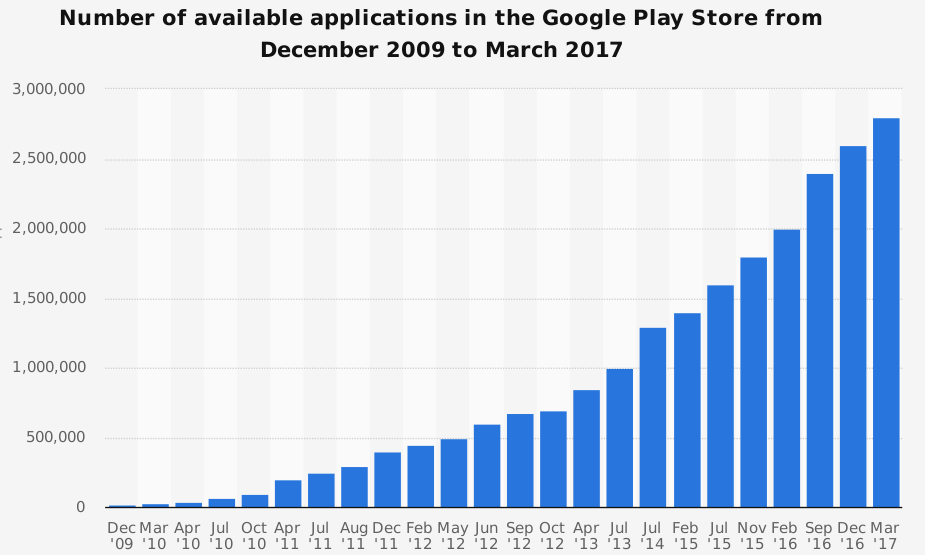
\includegraphics[width=0.8\textwidth]{Figures/ch1/introduction/google_play_number_of_apps}
  \caption{Crecimiento del número de aplicaciones disponibles en la tienda de Android, el sistema operativo para smartphones con más volumen de terminales en uso. \cite{GooglePlayApps}.}
\end{figure}

\section{Plataformas móviles: Android, iOS y el resto.}

Si dejamos a un lado la batalla entre los fabricantes de hardware (Samsung, LG, Sony, \ldots), nos encontramos con otra batalla en lo referente a la plataforma o sistema operativo utilizado.

En un principio, cada fabricante de teléfonos tenía su propio sistema operativo, el cual incluía en sus dispositivos. Además, eran los propios fabricantes los encargados de desarrollar las aplicaciones que se ejecutarían en sus terminales, lo que limitaba en gran medida la variedad de estás aplicaciones.

Mas tarde, diferentes fabricantes empezaron a unirse para crear conjuntamente sistemas operativos que compartían. El más famoso sin duda alguna fue Symbian. Este sistema operativo, propiedad de Nokia, fue producto de la alianza de esta con otras compañías como Siemens, Samsung, LG, \ldots pero fue Nokia la que más partido le saco y con la que se hizo famoso el sistema. Uno de los puntos fuertes de Symbian fue la gran comunidad de desarrolladores que realizaban aplicaciones para esta plataforma, lo que la hacía muy atractiva para un usuario final que, hasta entonces, apenas disponía de tonos y fondos de pantalla para personalizar su terminal.

Fue en 2007 cuando ocurrió un evento muy importante. La compañía Apple, ya famosa por sus ordenadores y su iPod, presento Iphone OS, que más tarde pasaría a llamarse \emph{iOS}, su nombre actual. Junto con el nuevo sistema aparecía el primer iPhone, el smartphone que sin duda supuso el inicio del \emph{boom} de este tipo de dispositivo. Este sistema es propietario de Apple, y solo lo podemos encontrar en sus terminales iPhone e iPad. Sus aplicaciones empezaron siendo escritas en Objective-C, lenguaje que años más tarde cambiaron para utilizar Switch. Este es un dato importante para lo que explicaremos a continuación.

Un año más tarde, allá por septiembre de 2008, Google presenta su sistema operativo, Android. Este sistema operativo estaba realizado por una empresa del mismo nombre, la cual Google había comprado unos años antes. La versión más básica es conocida como \gls{AOSP}, que se trata de un proyecto de código abierto. A diferencia de iOS, podremos encontrar Android en multitud de dispositivos de multitud de fabricantes, desde smartphones a encontrarse instalado en sistemas multimedia para automóviles, desde Samsung a BQ. En el caso de Android las aplicaciones están escritas usando Java.

El carácter abierto de Android ha propiciado que aparezcan diversos firmwares basados en él. Quizás los más conocidos sean MIUI\footnote{\url{http://en.miui.com/}}, propio de los terminales de Xiaomi, y el ya descontinuado CyanogenMOD. Pero por la web, podemos encontrar multitud de versiones y personalizaciones del sistema creada por la comunidad de desarrolladores. También es común que los fabricantes de smartphones que usen Android, creen su propia versión personalizada de este.

Junto a estos dos sistemas operativo han convivido otros como el ya mencionado Symbia, Windows y BlackBerry (que tuvo una época dorada allá por 2008). También intentos menos exitosos, como Fire OS de Amazon, Firefox OS (basado en HTML5) o Ubuntu Touch de Canonical. Pero si algo tienen en común todos ellos, es que se han convertido, o no han pasado de serlo, en sistemas operativos residuales en cuanto a cuota de mercado. En la siguiente tabla podemos ver esta cuota en el tercer cuatrimestre de 2016.

\begin{figure}[H]
\centering
  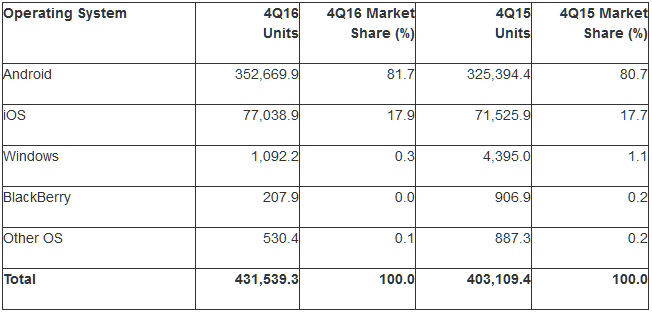
\includegraphics[width=\textwidth]{Figures/ch1/introduction/smartphone_sales_3q_2016}
  \caption{Cuota de mercado en el cuarto cuatrimestre del año 2016 según la plataforma. \cite{SmartPhonesSales}.}
\end{figure}

Otro dato curioso para ver la importancia que han tomado estos sistemas operativos y este tipo de dispositivos, es comparar el número de dispositivos conectados  a internet según su sistema operativo a lo largo del tiempo. En la siguiente gráfica se puede ver como peso de Windows para PC disminuye en tanto que el de los sistemas operativos para terminales móviles crecen.

\begin{figure}[H]
\centering
  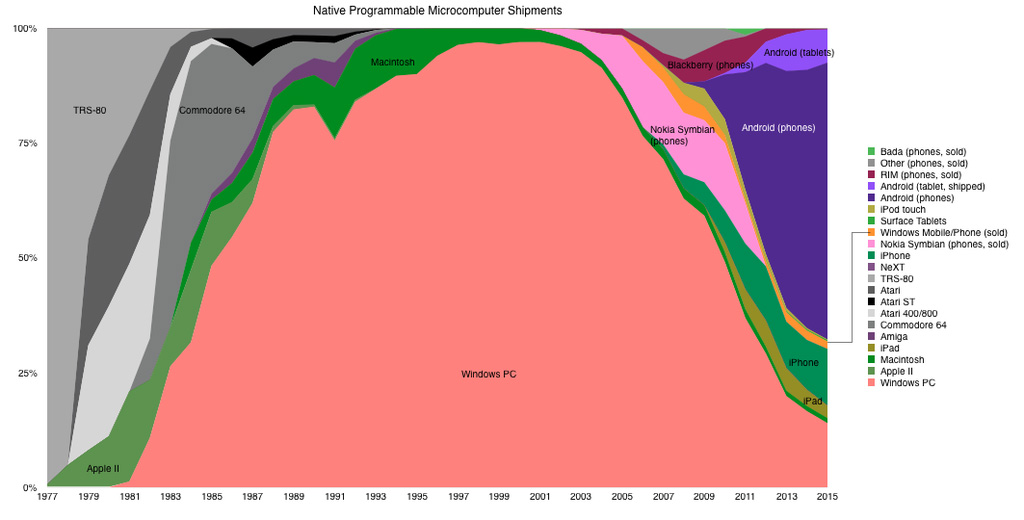
\includegraphics[width=\textwidth]{Figures/ch1/introduction/os_quota}
  \caption{Distribución de los dispositivos conectados a internet teniendo en cuenta el sistema operativo que utilizan.  \cite{PlatformsWar}. }
\end{figure}

\subsection{¿Un nuevo contendiente?. Google Fuchsia.}

\cite{Fuchsia} En el momento de escribir esta memoria (10 de mayo de 2017), se filtrado el que posiblemente sea un nuevo sistema operativo creado por Google. Este sistema vendría a unificar los dos sistemas operativos de la compañía, Android y Chrome OS\footnote{\url{https://www.chromium.org/chromium-os}}.

Las mayores características de este nuevo sistema serian por un lado, el abandono del kernel de linux del que hacen uso tanto Android como Chrome OS. Este sería remplazado por un kernel desarrollado por Google y que responde al nombre de Magenta. La otra diferencia sería el uso de Flutter SDK\footnote{\url{https://flutter.io/}}, un \gls{SDK} también desarrollado por Google para la creación de aplicaciones multiplataforma que se centra en el rendimiento y que utiliza el lenguaje Dart\footnote{\url{https://www.dartlang.org/}} (una alternativa a JavaScript lanzada por Google). Este \gls{SDK} aun se encuentra en sus primeras fases de desarrollo, pero de ser usado en el nuevo sistema, significaría que las aplicaciones creadas para Fuchsia, podrían ser también usadas en Android. En la web de Flutter SDK podemos encontrar una aplicación no funcional válida para Android en la que podemos ver una pequeña muestra de la UI que ofrece, la cual es conocida con el nombre de Armadillo.

Aun es pronto para saber los planes que tiene Google con este sistema operativo, y que hará con Android. Pero podemos encontrarnos con que en un futuro próximo se una esta nueva plataforma a Android y a iOS, diversificando más el mercado. Y es que aunque Google apueste por el nuevo sistema, serán los fabricantes de smartphone los que tendrán que introducirlos en sus dispositivos, y como se comento anteriormente, muchos de ellos cuentan con versiones personalizadas. Esto hará que el paso de Android a Fuchsia (en el caso de que se produzca) se alargue en el tiempo y ambas plataformas convivan.

\section{En la variedad está problema. Aplicaciones híbridas.}

A la hora de implementar una aplicación nos encontramos con el dilema de, ¿a qué dispositivo va dirigido?. Viendo las cuotas de mercado, se podría pensar que la opción mejor es lanzarse a crear nuestra aplicación para Android. Pero si investigamos un poco, veremos que las aplicaciones lanzadas en iOS producen hasta cuatro veces más beneficios que las de Android \cite{AndroidiOSRevenue}. Por otro lado, lo más probable es que no nos interese desarrollarla solo para iOS ya que Android cuenta con 7 veces más usuarios. También tenemos que pensar en la función que va a tener nuestra aplicación. Si por ejemplo, nuestra aplicación se basa en recoger datos de cualquier tipo (por ejemplo, reportar accidentes de tráfico) y compartirlos entre usuarios de la aplicación, nos interesa que nuestra aplicación llegue al mayor número de usuarios posible para poder captar un volumen mayor de datos. O si nuestra aplicación forma parte de un producto, como puede ser manejar un drone, no podemos excluir a una parte de potenciales compradores del producto únicamente por no disponer de un terminal que le permita ejecutar nuestra aplicación. Y no nos olvidemos de Windows \ldots

Como vemos, parece más que recomendable abarcar al menos las dos plataformas mas importantes a la hora de crear una aplicación, pero no siempre se cuenta con los recursos o conocimientos necesarios para abordar dos proyectos diferentes y no solo eso, si no también mantenerlos.

Para solventar este problema surgieron las \emph{aplicaciones híbridas}, ¿para qué programar dos aplicaciones desde cero si van a tener un mismo funcionamiento?. Mientras que las \emph{aplicaciones nativas} se desarrollan en el lenguaje específico de cada plataforma y utilizando la \gls{API} propia de cada sistema, las aplicaciones híbridas utilizan tecnología web (HTML5, CSS y JavaScript) para crear la aplicación y a continuación, mediante el uso de diferentes herramientas, son compiladas lo que genera un ejecutable para cada una de las plataformas.

Las aplicaciones hibridas nos ofrecen ventajas sobre las nativas, pero también presentan sus desventajas. En internet se pueden encontrar multitud de comparativas entre ambos tipos de aplicaciones y según el autor, las diferencias entre ellas serán mas o menos importantes. aún así, a continuación expondré aquellos puntos que considero más importantes a la hora de decidir por que tipo de aplicación apostar.

\paragraph{Curva de aprendizaje} En el caso de las aplicaciones nativas, debemos aprender como funcionan estas en cada una de las plataformas, el lenguaje que se utiliza para programar, las APIs que ofrece el sistema, \ldots en cambio, para las aplicaciones híbridas, solo será necesario saber HTML, CSS y JS junto con el framework o herramientas que utilicemos para ayudarnos a crear nuestras aplicación. Además, los frameworks que han aparecido para ayudar en la creación de aplicaciones híbridas facilitan mucho el trabajo con algunas de las \glspl{API} del sistema operativo, llegando a ser más fácil utilizarlas a través del framework, que de manera nativa. Este es el punto fuerte de las aplicaciones híbridas.

\paragraph{Diseño de la aplicación} Aunque cada vez son más y mejores los frameworks que nos ayudan a crear las aplicaciones híbridas, es cierto que en el desarrollo de este tipo de aplicaciones es más complicado el tener un diseño acorde a la plataforma. Puede parecer un problema menor, pero el aspecto de una aplicación es muy importante, y la experiencia de uso puede verse perjudicada al utilizar ciertos estilos a los que el usuario no esta acostumbrado (widgets, botones, distribución de elementos, \ldots). El problema puede ser aún mayor si la aplicación esta destinada para iOS, ya que Apple puede vetarla de su market si no cumple con ciertos estándares de diseño.

Puede parecer desproporcionado este énfasis en cuanto a la homogeneidad del diseño, pero si pensamos en los ordenadores de sobremesa, ocurre lo mismo. Por ejemplo, los usuarios de Windows estamos acostumbrados a que los botones para minimizar/cerrar una ventana se encuentren en la esquina superior derecha y sería complicado adaptarse a que eso no fuera así. Solo hay que ver las críticas que recibió Microsoft cuando lanzo Windows 8 con su menú, teniendo que volver a uno más tradicional en la versión 8.1.

\paragraph{Rendimiento de la aplicación} Otro punto en contra de las aplicaciones híbridas es el rendimiento. Suelen mostrarse más lentas que las nativas. Este problema puede no ser crítico en función del tipo de aplicación y si tenemos en cuenta que cada vez los dispositivos móviles son más potentes. Aun así, es un punto a tener en cuenta.

\paragraph{Seguriad} Por norma general, las aplicaciones nativas son más seguras que las hibridas. No nos olvidemos que estas últimas suelen hacer uso de frameworks que en su mayoría son libres y su código es abierto, lo que facilita la búsqueda de debilidades. Esto hace que su uso sesa poco recomendable en aplicaciones sensible, como por ejemplo aquellas que gestionen cuentas bancarias.

\paragraph{Disponibilidad de las capacidades del terminal} Es posible que no tengamos acceso (o esté limitado) a ciertas capacidades del dispositivo, por ejemplo, algún sensor en concreto, desde una aplicación híbrida. Evidentemente, este problema no lo tendremos con una aplicación nativa. Es por tanto importante comprobar que la tecnología que elijamos cubra nuestras necesidades, y no encontrarnos con esta limitación a mitad del desarrollo lo que conllevaría un esfuerzo extra \textbf{MUY} importante.

\paragraph{Costes} El factor que suele tener (lamentablemente) más peso a la hora de elegir. Es evidente que, una aplicación hibrida tiene un menor coste, ya que no requiere el dedicar un equipo de trabajo para cada plataforma. Incluso teniendo que implementar la aplicación para solo una, es muy posible que la aplicación híbrida sea una opción más económica (y deja la puerta abierta a ser lanzada en otras plataformas en el futuro).

En resumen, las aplicaciones hibridas son una buena alternativa para la mayoría de aplicaciones de hoy en día, y con la evolución de los framework, cada vez más. Pero si queremos una aplicación robusta, con una interfaz cuidada y un rendimiento óptimo, y siempre que el presupuesto lo permita, la opción nativa sigue siendo la más indicada.

Una buena estrategia es utilizar aplicaciones híbridas en la etapa inicial de nuestro proyecto y según cómo responda el mercado a nuestra idea, decidirse a dar el paso y hacer el cambio a aplicaciones nativas, eso sí, siempre que sea necesario.

\subsubsection{Frameworks al rescate}

Para ayudar al desarrollo de aplicaciones hibridas han surgido frameworks que facilitan la tarea de integración de las diferentes plataformas haciendo que converjan en una única interfaz.

Sin duda alguna, el proyecto que más ha impulsado la creación de aplicaciones híbridas  ese a sido Adobe Cordova (como veremos más adelante, también conocido como PhoneGap), que proporcionan las herramientas necesarias para que nuestra aplicación basada en tecnología web pueda ser ejecutada en el dispositivo. Junto con Cordova, han aparecido multitud de frameworks, algunos de los cuales utilizan Cordova como base, los cuales facilitan el desarrollo ofreciendo conjuntos de componentes estéticos, añadiendo patrones de programación, potenciando las tecnologías web usadas (\gls{HTML}, \gls{CSS} y \gls{JS}), \ldots.

\chapter{Marco Tecnológico}

En este capítulo vamos a ver el estado de las tecnologías relacionadas con las aplicaciones híbridas, haciendo mención de aquellas más importantes. A continuación, se verá con más profundidad aquellas que se usarán a lo largo de este \gls{PFC}, y que son Ionic, Angular y Cordova.

\section{Frameworks}

Al comienzo de la aparición de las aplicaciones web, los desarrolladores disponían únicamente de \gls{HTML}, \gls{JS} y \gls{CSS} para su implementación, sin ningún tipo de librería ni framework que les facilitará esta tarea. Se conoce como \emph{Vanilla JavaScript} al uso de JavaScript sin ningún tipo de librería ni framework. Con el aumento tanto en número como en complejidad de estas aplicaciones, se hizo necesario disponer de herramientas que facilitarán el desarrollo de estas.

Así comenzaron a surgir diferentes herramientas y frameworks que facilitaban las tareas de programación tanto en el lado de la lógica de negocio como en el apartado visual.

\subsection{jQuery}

jQuery\footnote{\url{https://jquery.com/}} fue y sigue siendo una de las librerías más usada en el mundo del desarrollo web. Esta librería tiene como objetivo facilitar algunas de las deficiencias que nos encontramos a la de programar con JavaScript.

Con jQuery conseguimos simplificar el acceso a los nodos del árbol \emph{DOM} que el navegador crea a partir de nuestro \gls{HTML}, consiguiendo una sintaxis mas clara, fácil de recordar y además compatible con todos los navegadores. Por ejemplo:

\begin{lstlisting}[style=htmlcssjs,frame=tlrb,xleftmargin={0.2cm}]
  // Vanilla JavaScript
  var elem = document.getElementById("miElemento");

  //jQuery
  var elem = \$("#miElemento");
\end{lstlisting}

También proporciona herramientas útiles como métodos específicos para realizar llamadas \emph{AJAX}, es decir, llamadas desde la aplicación web que se ejecuta en el navegador al servidor de manera asíncrona utilizando el protocolo \gls{HTTP}.

jQuery ha supuesto el punto de partida de muchos otros frameworks y complementos, lo que hace que tenga aún más valor. Ya que hablamos de la importancia de jQuery como base para otros proyectos, sería injusto no mencionar a \emph{underscoreJS}\footnote{\url{http://underscorejs.org/}}, otra librería que ha venido a suplir algunas cadencias de JavaScript.

Mas tarde, se lanzo jQuery UI\footnote{\url{http://jqueryui.com/}}, que consistía en un conjunto de herramientas y facilidades tanto CSS como JavaScript para la creación de interfaces de usuario. A su vez, de jQuery UI\footnote{\url{http://jquerymobile.com/}} surgió jQuery Mobile, una versión adaptada a dispositivos móviles que por aquella época empezaban cobrar mayor importancia.

\subsection{Framework CSS}

\cite{BootstrapFoundation,BestFramCSS} Con el paso de los años, el diseño de las páginas a ido haciéndose cada más y más complejo. Las diferentes versiones de \gls{HTML} y de \gls{CSS} han ido introduciendo nuevas opciones en este sentido, lo que aún siendo necesarias, a veces resultan insuficientes en el desarrollo de la página. Además de esto, la variedad de terminales desde los que se puede visualizar una página es también cada vez mayor, teniendo que pensar en el diseño según sea vista en un dispositivo móvil, una tablet, un PC, el navegador que se utiliza (ya que todos no reconocen los mismos parámetros), \ldots y no solo eso, también el tamaño de pantalla, la resolución, la orientación, \ldots. Si conseguimos que nuestro diseño se adapte a todos estos casos, podremos decir que el nuestro se trata de un diseño \emph{responsive}. Como nos podemos imaginar, el realizar un diseño \emph{responsive} requiere una cantidad de tiempo y recursos importante, ya que no solo debemos de implementar el estilo para diferentes usos, también es necesario probarlo.

Esta tarea de diseño ha sido facilitada con la aparición de lo que se conocen como \emph{frameworks \gls{CSS}}. Estos frameworks utilizan hojas de estilos creadas y testadas por equipos de desarrolladores y diseñadores con gran experiencias, listas para ser usadas como base en una maquetación web y no tener que partir desde cero. Una de la funcionalidades principales que suelen ofrecer, y que siempre a sido un dolor de cabeza para los diseñadores, razón por la que la destaco, son los \emph{grid}. Gracias ellos podemos dividir nuestra página en una especie de cuadrícula y sobre la que poder distribuir los elementos de nuestra página.

Aunque las ventajas de usar uno de estos frameworks son evidentes, también tienen ciertos inconvenientes a tener en cuenta antes de decidirnos a usarlos. En primer lugar es la limitación a la hora de personalizar el diseño, ya que partimos de uno ya creado y pensado para dar soporte a una gran cantidad de dispositivos, por lo que su implementación es compleja y modificarlo suele ser complicado. Otro inconveniente es el código del mismo framework. Lo más normal es que no se utilice todo lo que te ofrece el framework, pero aun así, será descargado por completo por el cliente. Según el tamaño y la conexión del cliente, esto puede ser un problema el cual, con la mejora de las conexiones, cada vez es menos importante.

\tipbox{
  Este tipo de frameworks suelen ofrecer un único núcleo y módulos separados los cuales implementan diferentes características. Así, podemos importar solo aquellos módulos que nos interesan, por ejemplo, el widget para el calendario o el módulo que maneja las tablas. También cuentan con versiones reducidas en los que el código esta ofuscado, consiguiendo reducir aún más el tamaño del código.
}

También tenemos que tener en cuenta la dificultad de aprendizaje de estos frameworks, lo que puede hacerlos poco atractivos para pequeños proyectos si no tenemos conocimientos y experiencia previa con ellos.

El anteriormente mencionado jQuery UI se considera un framework \gls{CSS}, pero han surgido durante los últimos años otros más potentes y más interesantes. Actualmente los dos más importantes se podría decir que son:

\begin{enumerate}
  \item Bootstrap\footnote{\url{getbootstrap.com}}: Desarrollado por Twitter, quien lo liberó como código abierto más tarde, se trata del framework \gls{CSS} más conocido y utilizado, siendo uno de los proyectos con más apoyo en Github\footnote{\url{https://github.com/}}. Se puede observar en la gráfica de debajo de estas líneas la diferencia de interés que despierta en comparación con Foundation, el otro gran framerwork \gls{CSS}, si tenemos en cuenta las búsquedas realizadas en Google. Sus puntos fuertes son su preocupación por la compatibilidad y la estabilidad (realizan test automáticos antes de publicar cualquier cambio en la rama principal del repositorio\footnote{\url{https://github.com/twbs/bootstrap}}), su sistema de \emph{Grid} y la gran comunidad que hay detrás. En su última versión utiliza tecnologías recientes como \gls{Sass}, implementan \emph{Flexbox} de \gls{CSS}, usan \glspl{mixin}\footnote{\url{http://getbootstrap.com/css/#mixins}} y hojas de estilos separadas para mejorar la escalabilidad \ldots.

  \begin{figure}[H]
\centering
    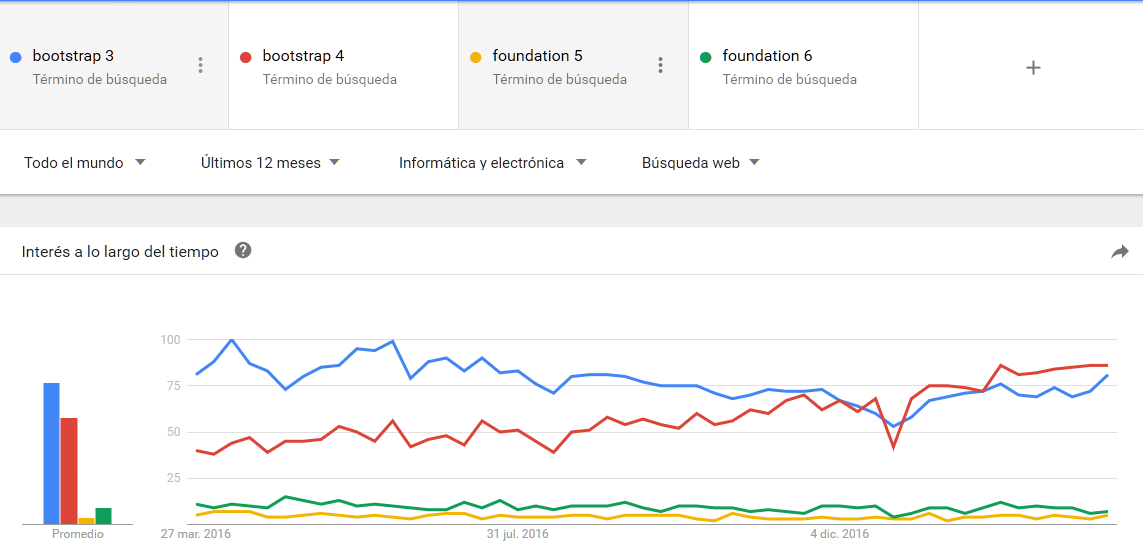
\includegraphics[width=0.8\textwidth]{Figures/ch1/frameworks/graph_frameworks_css}
    \caption{Busquedas mundiales de los dos frameworks CSS más importantes.}
  \end{figure}

  \item Foundation\footnote{\url{http://foundation.zurb.com/}}: Nos encontramos ante un framework que, aunque menos usado y apoyado, cuenta con una potencia similar a lo visto en Bootstrap. Al igual que este, hace uso de \gls{Sass}, \emph{Flexbox}, \glspl{mixin}, \ldots además de un sistema de \emph{Grid} considerado mejor que el de Bootstrap. Palidece, eso sí, si hablamos de compatibilidad y de estabilidad. Cuenta con una integración especial para \textbf{emails}, por lo que lo hace muy recomendable en caso de que nuestro diseño se tenga que adaptar al envío de correos. Todo esto hace que sea una alternativa igual de valida que Bootstrap.
\end{enumerate}

Aunque estos son los más importantes, existen otros muchos framework los cuales merece la pena mencionar como es Pure.CSS\footnote{\url{https://purecss.io/}}, cuya fuerza radica en su ligereza y sencillez, o Materialize\footnote{\url{http://materializecss.com/}}, enfocado en el estilo \emph{material design}.

\subsection{Framework Javascript}\label{subsec:frameworkJS}

 \cite{FramJSComp} Al igual que ha ocurrido con el diseño de las páginas, la lógica de negocio que se implementa en estas también a aumentado en complejidad. Se ha producido además un incremento de popularidad de las aplicaciones \gls{SPA}. En el desarrollo de este tipo de aplicaciones, trabajar solo con JavaScript se hace sumamente complicado, y  jQuery por si mismo no llega a cubrir todas las necesidades que iban surgiendo. Se hacia patente por tanto la necesidad de disponer de herramientas que facilitaran el desarrollo de estas páginas.

Estos framework proporcionan multitud de facilidades, pero hay que ser cauto a la hora de elegir uno y usarlo para nuestro proyecto. Se debe tener en cuenta el tiempo de aprendizaje que requiere y que se deber sumar, además del propio tiempo de implementación. Si además, la aplicación va a tener que ser mantenida y va a sufrir actualizaciones, debemos de asegurarnos de que el framework elegido vaya a gozar de un buen futuro y que tendremos los conocimientos suficientes para abordar el proyecto con el framework escogido, de no ser así, correremos el riesgo de tener que enfrentarnos en el futuro con la deuda técnica que una mala decisión puede provocar.

Empezaron entonces a surgir multitud de frameworks muchas características en común: son de código abierto, implementan patrones de diseño tipo \gls{MV*} con los que intentan solventar los problemas de las \gls{SPA}; todos ellos manejan los conceptos de vista, evento, modelo y ruta.

Sin mencionar Angular, del cual hablaremos más adelante con más profundidad, destacan:

\begin{enumerate}
  \item Backbone.js\footnote{\url{http://backbonejs.org/}}: Fue uno de los más populares y usados antes de la explosión de Angular. Este framework que implementa el patrón \gls{MVC}, permite utilizar el sistema de plantillas que se quisiera, usar otras librerías, \ldots. Además, y a pesar de tratarse de un framework bastante potente, destaca por su reducido tamaño, de apenas unos 7 Kb. Este framework es muy recomendable para proyectos de pequeño tamaño y poco complejos, ya que en aplicaciones grandes con cierta complejidad, la carecía de ciertas facilidades con las que otros frameworks cuentan se hace más evidente.
  \item Knockout.js\footnote{\url{http://knockoutjs.com/}}: Como el anterior, se trata de un framework muy ligero, apenas 40 Kb, pero que ofrece soluciones muy interesantes y diferenciadoras como el uso del patrón \gls{MVVP}, el poder hacer un binding entre los datos y los elementos del árbol \gls{DOM} o su sistema de plantillas. Al igual que ocurría con Backbone.JS, este framework no es muy recomendable para su uso en aplicaciones de cierto tamaño y complejidad.
  \item Ember.js\footnote{\url{https://emberjs.com/}}: Otro framework relativamente joven y que implementa el patrón \gls{MVC}. Está basado en jQuery y HandlebarsJS \footnote{\url{http://handlebarsjs.com/}}, por lo que ambas librerías deben ser importadas en nuestra página. Su filosofía es hacer que el código sea lo mas limpio y sencillo posible, lo que es conocido como \emph{Ember way}. Se basa en el paradigma de programación de \textbf{Convención sobre configuración} en su busqueda de la simplicidad. Este empeño por la simplicidad hace que sea menos flexible que otros framework. A parte de eso, implementa otras facilidades como \emph{routing}, \emph{binding}, funcionalidades para trabajar con APIs RESTful, \ldots
  \item React \cite{ReactJSEMACSScript}: A decir verdad, no es del todo correcto incluir React en esta lista ya que no se trata de un framework como los anteriores, si no que se trata de una librería de JavaScript, pero he decidido incluirla aquí debido a la popularidad que está consiguiendo últimamente. Facebook se encuentra detrás del desarrollo y mantenimiento de esta librería que esta enfocada en el renderizado de la página, se puede decir que es la \textbf{V} del patrón \gls{MVC}. Es por esto que puede ser usado junto otros frameworks que se encarguen de otras funciones del patrón, como por ejemplo, con Angular. Está basado en componentes, los cuales controlan su propio estado y cuya lógica se encuentra implementada en el JavaScript. Su característica más importante es el DOM virtual que genera con cada componente y el algoritmo \emph{Diff} que le permite a la hora de producirse un cambio, calcular solo la parte del DOM a la que afecta este cambio, y solo repintar esta parte. Con esto se consigue que el tiempo de renderizado disminuya considerablemente.
\end{enumerate}

\tipbox{La palabra \textbf{renderización} es una adaptación al castellano del vocablo inglés "rendering" y que define un proceso de cálculo complejo desarrollado por un ordenador destinado a generar una imagen o secuencia de imágenes.}

Podemos comparar el interés que despiertan estos frameworks usando la herramienta Google Trends:

\begin{figure}[H]
\centering
  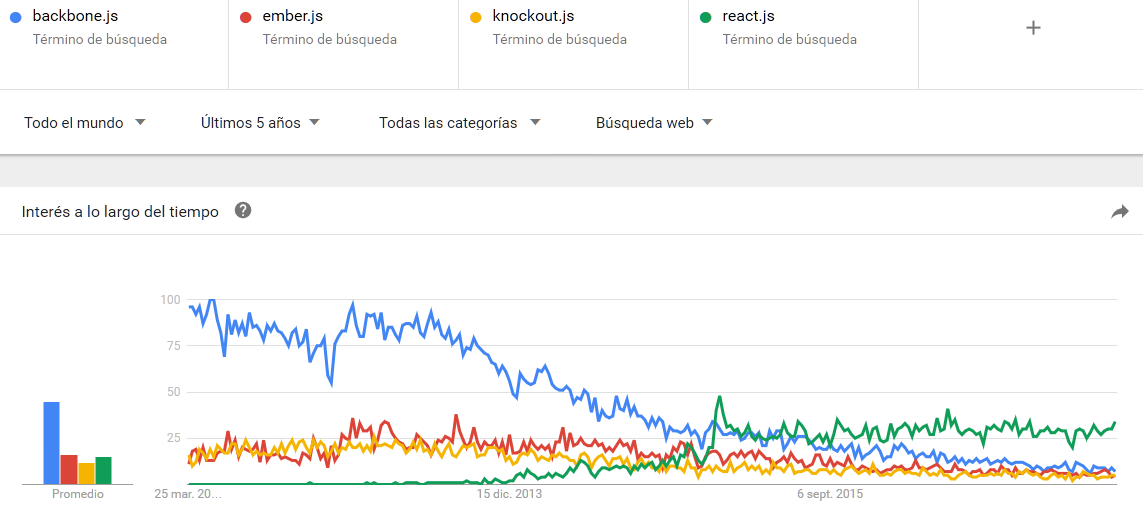
\includegraphics[width=0.8\textwidth]{Figures/ch1/frameworks/graph_frameworks_js_wo_angular}
  \caption{Evolución de las busquedas en Google de los diferentes frameworks.}
\end{figure}

Vemos como hace unos años Backbone.js gozaba de gran popularidad, estando claramente por encima del resto, pero  poco a poco esta popularidad ha ido bajando hasta ponerse al nivel de Knockout.js y EmberJS, los cuales mantienen más o menos el nivel pero también sufren. Por el contrario, React.js, aun siendo el último en llegar, consigue superar a los anteriores. Uno de los motivos de estas variaciones es la evolución que están teniendo las \gls{SPA} y las aplicaciones híbridas. Vemos como Backbone.js y Knockout.js son los que mas han bajado y son a su vez, los menos eficaces para desarrollar páginas complejas.

Si os preguntéis por qué no he añadido Angular al gráfico anterior, debajo de esta línea podéis ver la razón.

\begin{figure}[H]
\centering
  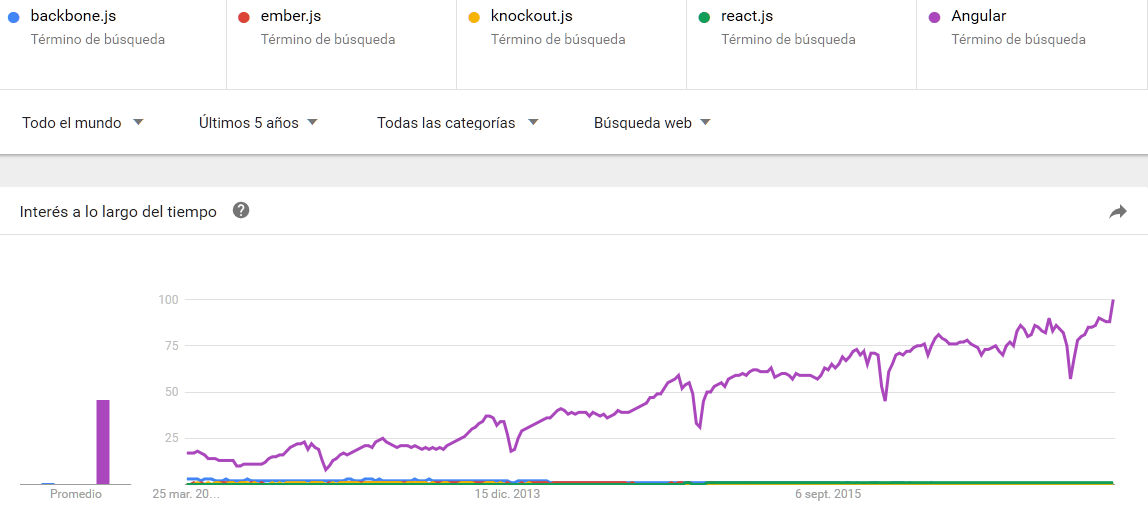
\includegraphics[width=0.8\textwidth]{Figures/ch1/frameworks/graph_frameworks_js_w_angular}
  \caption{La diferencia con Angular es tal, que impide ver correctamente los datos del resto de frameworks.}
\end{figure}

\subsection{Frameworks para aplicaciones híbridas}

\cite{Top10FramHybApp,TopFramHybApp} Junto a la aparición de las aplicaciones híbridos han ido aparecido nuevas necesidades. Como se ha visto en la \nameref{ch:introduction}, el fuerte de estas aplicaciones es la posibilidad de crear una aplicación que funcione en diferentes tipos de dispositivos a partir de un único desarrollo. La variedad de dispositivos, no solo si tenemos en cuenta la plataforma en la que se basa, si no también las características del hardware (en especial el tamaño y la resolución de la pantalla) puede suponer un problema a la hora de realizar el diseño de nuestra aplicación. Por otro lado, este tipo de aplicaciones suelen tener cierta complejidad, ya que suelen estar compuestas por diferentes vistas, utilizan servicios en la nube, necesitan comunicarse con la \gls{API} del dispositivo, \ldots.

Surgieron entonces diferentes frameworks que tratan de dar solución a estos problemas. Algunos de ellos pensados para crear aplicaciones web que se vieran bien en los navegadores móviles, pero que se han usado a la hora de crear aplicaciones híbridas, y otros cuyo único objetivo es servir para el desarrollo de estas últimas. Obviando tanto \emph{Apache Cordova} como \emph{Ionic} ya que hablaremos de ellos más adelante, los más destacables son:

\begin{enumerate}
  \item jQuery Mobile: El abuelo de los framework para dispositivos móviles. Se trata de una versión mínima de jQuery UI y que como no, se apoya sobre jQuery. Se trata de un framework ligero cuyo objetivo principal es funcionar en el mayor número posible de terminales sin importar la plataforma, el tamaño o el navegador usado. Tiene su propio estilo, sin adaptarse al \emph{look and feel} de la plataforma que lo ejecuta, lo que es una limitación importante si queremos decidirnos por él. Aunque no lo incorpora por defecto, es compatible con Apache Cordova.
  \item Appcelerator Titanium: Este framework no sirve para crear aplicaciones híbridas tal como las hemos definido, pero es importante también nombrarlo debido a la popularidad con la que cuenta. A diferencia de \emph{Apache Cordova}, que como veremos más adelante, utiliza un una WebView sobre la cual corre la aplicación web, \emph{Appcelerator} traduce el código JavaScript al código nativo de la plataforma. La interfaz gráfica se crea desde el propio \gls{JS}. Solo se encuentran disponibles las plataformas Android y iOS, que aunque menor, puede ser un inconveniente en según que proyecto. Además, el código a utilizar en Android y en iOS presentan algunas diferencias, lo que nos puede llevar a a tener que mantener dos códigos, aunque con variaciones mínimas entre ellos.
  \item React Native: Este framework esta apoyado por Facebook, quien lo creo y libero hace unos años. React Native no se basa \emph{Apache Cordova} como hace \emph{Ionic}, si no que ejecuta el código \gls{JS} de la aplicación utilizando el motor Javascript de la plataforma (V8 en Android, Javascript Core en iOS) y a medida que se va ejecutando la aplicación, un interprete lee el código \gls{HTML} y crea una vista nativa según este. Esto le proporciona la ventaja de que los elementos que se ven en realidad son nativos, haciendo que se vean mejor que los que generan otros frameworks que se basan en "imitarlos" usando estilos \gls{CSS}.
  \item NativeScript: Similar a React Native en cuanto a funcionamiento, pero permitiendo además el uso de TypeScript y Angualar2 para programar nuestra aplicación y no tener que estar limitados al uso de ReactJS. Un inconveniente que tiene respecto a React Native es la empresa que está detrás. Mientras que ReactJS cuenta con Facebook a sus espaldas, NativeScript está soportado Telerik, que sin querer menospreciarles, no poseen el mismo empuje con el que cuenta el anterior.
  \item Framework 7: Por último nos encontramos con Framework 7, el cual se centra únicamente en iOS y en Android. Permite la creación de aplicaciones híbridas usando PhoneGap, o de WebApps, es decir, aplicaciones que se ejecutan en el navegador, pero manteniendo el aspecto visual de la plataforma donde se ejecuta.
\end{enumerate}

\tipbox{El término \textbf{look and feel} se refiere al aspecto y comportamiento que presenta una interfaz gráfica de cara al usuario. Por lo general, una aplicación o sistema cuentan con una serie de características visuales (paleta de colores, tipo y tamaño de letra, animaciones, iconos, \ldots) que el usuario es capaz de reconocer como propio de esta aplicación o sistema.}

Como en los anteriores frameworks, podemos comprobar la popularidad de los comentados según sus búsquedas en Google.

\begin{figure}[H]
\centering
  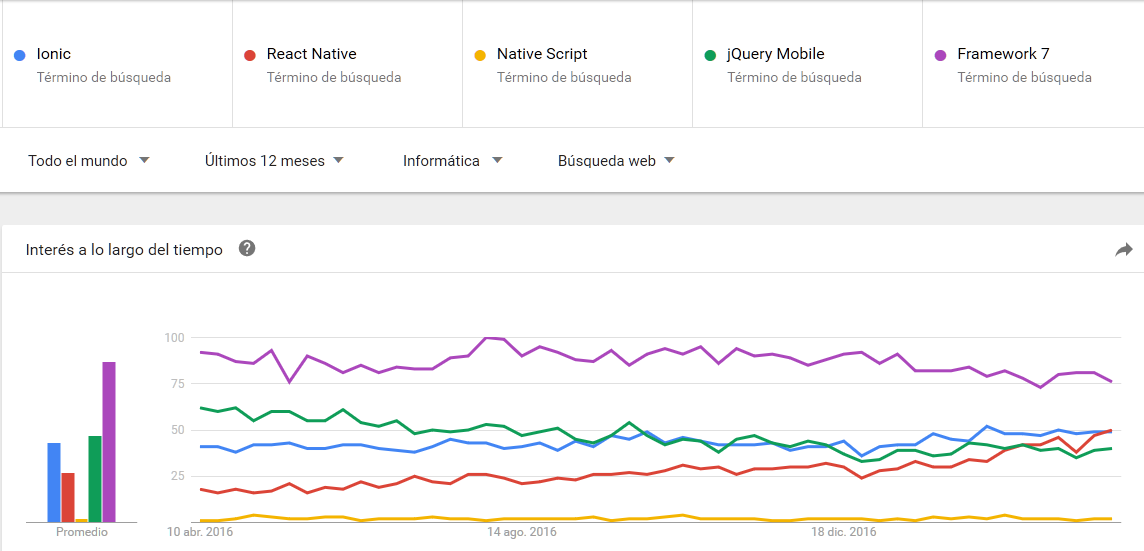
\includegraphics[width=0.8\textwidth]{Figures/ch1/frameworks/graph_frameworks_hyb}
  \caption{Vemos como quitando Framework 7 y NativeScript, el resto de frameworks están a la par.}
\end{figure}

Hay que decir que tanto Framework 7 como jQuery Mobile también son usados para la creación de WebApps y de paginas web con aspecto \emph{responsive}, por lo que cuentan con cierta ventaja a la hora de hablar de popularidad. Si miramos por foros y en diversas comunidades de desarrolladores, parece que las opciones preferidas a la hora de crear aplicaciones híbridas son Ionic y React Native.

\section{Angular}\label{sec:angular}

AngularJS\footnote{\url{https://angular.io/}} es un framework para JavaScript utilizado en la creación de aplicaciones web funcionales, también conocidas como aplicaciones de una sola página o en inglés \emph{Single Page Application}. Se trata de un framework de código abierto desarrollado y mantenido por Google. En los últimos años, AngularJS se ha convertido en un framework muy popular dentro de la comunidad de desarrolladores, siendo uno de los más utilizado.

\begin{flushright}
\emph{AngularJS is what HTML would have been, had it been designed for building web-apps. Declarative templates with data-binding, MVW, MVVM, MVC, dependency injection and great testability story all implemented with pure client-side JavaScript!}\\
Web del proyecto AngularJS.
\end{flushright}

AngularJS trata de traer el orden al código de nuestra aplicación. Para ello dispone de las facilidades necesarias a la hora de desarrollar para poder separar la lógica de negocio de la presentación. Se dice que el patrón de arquitectura que sigue es MVW o MV* (Model-View-Whatever!). También se consigue una mejora del rendimiento a la hora de usar AngularJS, entre otras cosas, debido a que no es necesario recorrer el árbol DOM como si que ocurre con otras librerías como \emph{jQuery}.

\begin{figure}
\centering
  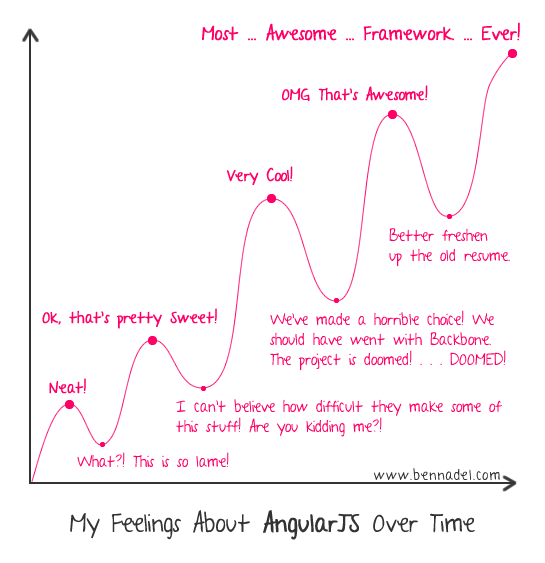
\includegraphics[width=0.8\textwidth]{Figures/ch1/angular/ben_nadel_experience_w_angular}
  \caption{El programador Ben Nadel describió (y de manera muy acertada) su experiencia con Angular en su blog de esta forma. \cite{AngBenNadel}}
\end{figure}

Como ya se vio en la sección \nameref{subsec:frameworkJS}, Angular se ha hecho muy popular siendo hoy en día el framework que goza de más popularidad con diferencia. Esto es importante a la hora de decidir si usarlo o no en nuestro proyecto, ya que nos garantiza el soporte durante los próximos años. Pero hay que tener en cuenta que se trata de un framework complejo, con una curva de aprendizaje que es necesario que tengamos también en cuenta.

Forma parte del stack \gls{MEAN}\footnote{\url{http://mean.io/}} junto con MongoDB, Express y Node.JS. Hablaremos de él mas adelante en el apartado \nameref{subsec:MEAN}.

\subsection{Angular versión 2}

\cite{SharifAng2} Y llego la conferencia europea de AngularJS de 2014 \ldots. En esta conferencia se dio la noticia de que se estaba desarrollando Angular 2.0 y que esta nueva versión sería incompatible con la primera y no habría una hoja de migración desde 1.x a 2.0. En Angular 2.0 se acaba con pilares de la versión tan importantes como es el \emph{\$scope} o los \emph{controladores}, que son sustituidos por los \emph{components}. Estos grandes cambios fueron muy criticados por la comunidad de desarrolladores, los cuales veían como todo lo aprendido iba a dejar der útil. Podemos decir por tanto que más que una segunda versión de AngularJS, se trata de un framework totalmente nuevo.

\tipbox{Angular, AngularJS, Angular2, \ldots ¿Cómo debemos de llamar a este framework?. Pues bien, se ha establecido que:
\begin{enumerate}
  \item Las versiones 1.x serán nombradas como \textbf{AngularJS}.
  \item Las versiones 2.x en adelante tomarán el nombre de \textbf{Angular} a secas.
  \item Se indicará el número de versión si se quiere mencionar a una característica concreta de esta. Por ejemplo, \textbf{Angular 2.4}
  \item La versión \gls{SEMVER} completa si queremos indicar algún bug.
\end{enumerate}}

\tipbox{En el momento de escribir esta memoria, acaba de salir la versión 4 de Angular. Esta nueva versión es compatible hacia atrás con la versión 2. También se anunciado la futurible versión 5.
El motivo de saltar de numeración del 2 al 4 es para unificar la versión de los paquetes del core de Angular ya que estos paquetes se distribuyen por separado y utilizan \gls{SEMVER}. Además, todos estos paquetes se encuentran en la misma versión que Angular excepto uno, \@angular/route, el cual se encuentra en la versión 3.x. Por ello, han decidido saltarse la versión 3 e ir directamente a la 4. }

Aunque Angular es perfectamente compatible con Vanila JavaScript, se recomienda el uso de TypeScript a la hora de programar nuestra aplicación. Gracias a TypeScript el desarrollo será mucho mas sencillo, además, el propio framework está escrito utilizando TypeScript, por lo que la compatibilidad es completa.

\subsubsection{TypeScript}

TypeScript\footnote{\url{https://www.typescriptlang.org/}} es un superconjunto de JavaScript, es decir, se trata de un lenguaje basado en JavaScript, al cuál le añade grandes beneficios. Es por esto que podemos usar código JavaScript en nuestro código TypeScript con la tranquilidad de que va funcionar correctamente. TypeScript implementa todas las funcionalidades que define ECMAScript 6\footnote{\url{http://es6-features.org/}}, añadiendo además algunas propias (algunas de las cuales se plantean introducir en ECMAScript 7).

Para que las aplicaciones escritas usando TypeScript puedan ser usadas en motores de ejecución de JavaScript, por ejemplo en los navegadores, la mayoria de los cuales reconocen ECMAScript 5, el código TypeScript debe ser compilado, lo que hace que sea traducido a JavaScript. Es este código traducido al JavaScript el que es realmente ejecutado por el navegador (o la WebView).

Algunas de las características (parte de las cuales son compartidas por los estándares mencionados antes) que TypeScript añade sobre JavaScript son:

\begin{enumerate}
  \item El uso de clases, haciendo del lenguaje un lenguaje orientado a objetos, lo que es de gran ayuda en proyectos de cierta envergadura.
  \item El tipado de variables y verificación en tiempo de compilación.
  \item Interfaces y herencia.
  \item Uso de anotaciones.
  \item Funciones lambda\footnote{\url{https://basarat.gitbooks.io/typescript/docs/arrow-functions.html}}.
  \item Uso de clases \emph{mixin}\footnote{\url{https://www.typescriptlang.org/docs/handbook/mixins.html}}
  \item \emph{Tuplas} y las \emph{Enumeraciones}.
  \item \ldots
\end{enumerate}

\subsubsection{Aspectos más importantes en Angular}

\cite{Ang2EnrOriol,DiffCompDir} Después del breve apunte sobre TypeScript, sigamos hablando de Angular. Sería necesario bastante más que un capítulo dentro del marco tecnológico de este \gls{PFC} para poder explicar en detalle todas las características que ofrece Angualar2. Por ello, vamos a centrarnos en comentar aquellas más relevantes y así estar algo más preparados a la hora de enfrentarnos a la realización de las prácticas más adelante. Como veremos, Angular se aprovecha de las \emph{clases}, las \emph{anotaciones}, la \emph{herencia}, \ldots que define TypeScript para implementar las funcionalidades que ofrece, por ejemplo, los \emph{componentes} o \emph{directivas} que explicaremos a continuación se implementan como clases con unos metadatos definidos mediante una anotación.

\begin{figure}[h]
\centering
  \includegraphics[width=\textwidth]{Figures/ch1/angular/Angular2_diagram}
  \caption{Esquema de algunos de los elementos que encontramos en una aplicación realizada con Angular y como interactúan entre ellos.}
\end{figure}

\paragraph{Módulos} Angular es modular. Se organiza en módulos los cuales se caracterizan por tener un único objetivo. Estos módulos  suelen exportar ciertos elementos que pueden ser usados por otros módulos. Un ejemplo de módulos serían las librerías que forman Angular y que debemos importar cada vez que queremos usar alguna de sus facilidades.

\notebox{
  Dentro de las librerías de Angular, las más importantes son:
  \begin{enumerate}
    \item @angular/core
    \item @angular/common
    \item @angular/router
    \item @angular/http
  \end{enumerate}
  Veremos el uso de algunas de ellas a lo largo de \nameref{ch:practices}
}

\paragraph{Components}

Una aplicación hecha con \emph{Angular} está formada por \emph{componentes} los cuales cuelgan uno de otros formando una especie de árbol. Existe un  \emph{component} raíz del cual cuelgan el resto de  \emph{componentes}. Esta estructura es similar a la que nos podemos encontrar en un \gls{HTML}, donde todos los elementos se encuentran anidados dentro de otro hasta llegar al elemento \textbf{<body>}.

Un componente está definido por una clase a la que se le añade la anotación \emph{@component}, donde se definen los metadatos del componente, y un \textbf{template} que define la vista (engloba el \gls{HTML} y el \emph{CSS}). Tanto las propiedades como los métodos definidos en un componentes son accesibles desde la vista. Un elemento del \gls{DOM} solo puede estar asociado a un componente.

Los componentes se utilizan para separar la aplicación en pedazos más pequeños.

\paragraph{Data Binding}

En mi opinión, una de las características más potentes de Angular. Gracias al \emph{Data Binding} que ofrece Angular, podemos conectar valores entre la vista y la parte lógica de nuestro componente y convertir acciones que realice el usuario en llamadas a métodos sin tener que escribir toda la lógica que hay detrás de esto.

\paragraph{Directivas}

Una directiva nos permite añadir comportamiento a un elemento \gls{DOM} ya existente. En realidad, los \emph{componentes} son \emph{directiva} con una vista asignada, mientras que una \emph{directiva} puede ser reusada en diferentes elementos del \gls{DOM}, además de poder usar varias sobre un mismo elemento.

Las directivas se definen utilizando la anotación \emph{@directive}, en el que también se definen los metadatos de la directiva.

\paragraph{Servicios}

Los servicios son clases con una funcionalidad específica y que es compartido por los componentes que forman la aplicación. Estos servicios son accesibles desde los diferentes componentes gracias al inyector de dependencias (\emph{Dependency Injection}). Para definir un servicio se utiliza el decorador \emph{@injectable}.

Un uso típico de los servicios es la recuperar datos desde una fuente externa para ser usados en nuestra aplicación.

\paragraph{Dependency Injection}

Este término hace referencia a un mecanismo para proporcionar nuevas instancias de una clase con todas aquellas dependencias que requiere, facilitando así la modularidad. Se utiliza sobretodo para inyectar los servicios a los componentes que los van a usar, y todo esto con solo especificar en el constructor del componente los servicios que espera.

A la hora de crear nuestra aplicación, debemos de indicar los servicios que se van a utilizar a través de un \emph{provider} definido en el módulo lo contiene. Así, el inyector sabe como debe instanciar las dependencias que le "soliciten" los diferentes componentes (u otros servicios).

\subsection{MEAN}\label{subsec:MEAN}

\cite{MEAN} Aunque esta sección está englobada dentro de \nameref{sec:angular}, no nos confundamos, es Angular la que en verdad forma parte del stack \gls{MEAN}\footnote{\url{http://mean.io/}}. Aunque no veremos nada sobre este a lo largo de este \gls{PFC}, y el único componente de los que esta formado y vamos a tratar sea Angular, me ha parecido interesante introducirlo mediante una breve introducción. Pero, ¿a qué nos referimos cuando hablamos del stack \gls{MEAN}?.

Se conoce como stack \gls{MEAN} al conjunto de tecnologías que permiten la creación de aplicaciones distribuidas utilizando únicamente, y en todas sus fases, JavaScript. El nombre se debe a que las cuatro tecnologías principales que lo forman, son \textbf{M}ongoDB, \textbf{E}xpress, \textbf{A}ngular y \textbf{N}odeJS. Esto no quiere decir que no se puedan usar otros elementos como Browser, Selenium, Sass, \ldots para facilitarnos el trabajo.

\begin{figure}[H]
\centering
  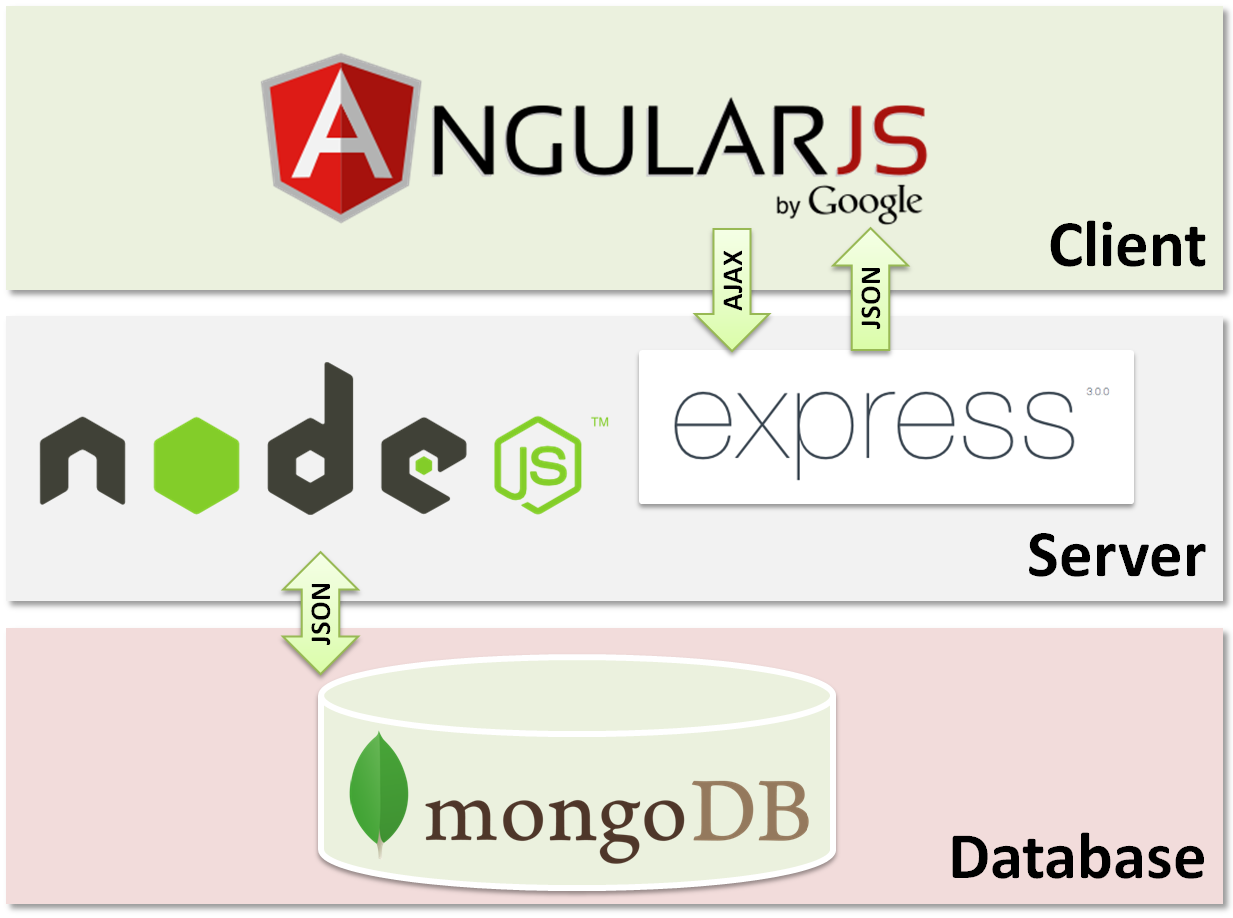
\includegraphics[width=0.8\textwidth]{Figures/ch1/angular/mean}
  \caption{Los cuatro elementos principales del stack en cada una de las fases.}
\end{figure}

\begin{enumerate}
  \item NodeJS: Un entorno de ejecución de JavaScript, basado a su vez en el motor de ejecución V8 desarrollado por Google. Este proyecto ha permitido que JavaScript de el salto del lado del cliente a poder ser usado también en la parte del servidor (aunque en sus inicios ya lo podíamos encontrar, pero no tuvo mucho recorrido). Provee de una arquitectura orientada a eventos (como la de los navegadores) así como una serie de APIs asíncronas que le proporcionan un rendimiento y una escalabilidad muy elevadas.
  \item Express\footnote{\url{http://expressjs.com/}}: Framework utilizado para implementar aplicaciones web sobre NodeJS. Aunque podemos crear nuestro servidor sin necesidad de utilizar ningún tipo de herramienta ajena a NodeJS, ExpressJS nos facilita esta tarea cubriendo las principales necesidades de cualquier servidor web (gestión de peticiones y respuestas, cabeceras, rutas, vistas, \ldots).
  \item MongoDB\footnote{\url{https://www.mongodb.com/}}: En la parte de almacenamiento se encuentra esta \gls{BBDD} \gls{NoSQL} de tipo documental, que almacena la información en un formato similar al \gls{JSON}.
  \item Angular: Utilizado como no podría ser de otra manera para implementar el cliente de la aplicación distribuida.
\end{enumerate}

La razón por la que se ha hecho esta pequeña introducción a \gls{MEAN} es por la importancia que está consiguiendo dentro de la comunidad de desarrolladores. JavaScript se esta posicionando como uno de los lenguajes principales, y herramientas como esta, hacen que su uso no se restrinja a solo el lado del cliente. Además, una aplicación móvil, y de esto si que trata el este \gls{PFC}, suele apoyarse en servidores, por lo que es conveniente saber que alternativas se encuentran disponibles para su implementación, y si es usando un lenguaje (JavaScript) y una tecnología(NodeJS) ya conocida, mejor.

\notebox{
  Por mi experiencia en el desarrollo de aplicaciones distribuidas, recomendaría a un desarrollador sin experiencia en backend empezar con un framework más estructurado y robusto, como puede ser Django (framework para Python), y una vez que se tiene un poco de experiencia, dar el salto (si se quiere) al uso tecnologías relacionadas con NodeJS.
}

\section{Apache Cordova}

Apache Cordova, o Cordova a secas, se trata de un entorno de desarrollo de aplicaciones móviles utilizando tecnologías web, \gls{HTML} y \gls{CSS} para la presentación, \emph{JavaScript} para la lógica. Es posible que hayas escuchado hablar sobre algo llamado \emph{PhoneGap}, pues bien, antes de continuar, convendría explicar que relación existe entre ambos. Si nos remontamos a 2008, una empresa llamada \emph{Nitobi} presenta PhoneGap, un entorno para la creación de aplicaciones móviles usando tecnologías web (de momento no hay diferencias con Cordova). En 2011 deciden donar el código a la fundación \emph{Apache}, lo que supone que se convierta en software libre, y debido al éxito que tiene, ese mismo año, \emph{Adobe} compra \emph{Nitobi}, quedándose con sus empleados, sus proyectos, sus marcas, \ldots y dentro de este paquete se encuentra PhoneGap. Decide entonces mantener PhoneGap como software Open Source, pero debido a que la marca PhoneGap pertenece a \emph{Adobe}, optan por cambiarle el nombre, surgiendo así Apache Cordova\footnote{\url{https://www.campusmvp.es/recursos/post/PhoneGap-o-Apache-Cordova-que-diferencia-hay.aspx}}. Así que como vemos, ambos proyectos se tratan del mismo. La única diferencia destacable es el servicio \emph{Adobe PhoneGap Build}\footnote{\url{https://build.phonegap.com/}}, que nos permite compilar nuestro código en la nube a cualquier plataforma sin necesidad de tener que tener instalado en nuestro ordenador la SDK de cada plataforma. Entonces, ¿Cuál debemos usar?. Cualquiera de los dos, al final, se trata de lo mismo. Lo único a tener en cuenta es si vamos a usar alguno de los servicios que ofrece Adobe.

Tras esta breve explicación, necesaria ya que siempre surge la duda, veamos como funciona Cordova. El objetivo es conseguir que nuestro código realizado con tecnologías web sea ejecutado en cualquier plataforma como si de una aplicación nativa se tratase. Para conseguir esto, Cordova proporciona un entorno nativo para cada plataforma sobre el cual, se ejecutará nuestra aplicación. Esta envoltura está compuesta por un navegador (WebView) que se encarga de ejecutar nuestro código, y si son necesario, una serie de plugins que permiten la comunicación entre nuestro código y las \glspl{API} de cada plataforma a través de una \gls{API} unificada. Estos plugins pueden ser ofrecidos por el propio Cordova, como ser realizados por terceros.

\begin{figure}[H]
\centering
  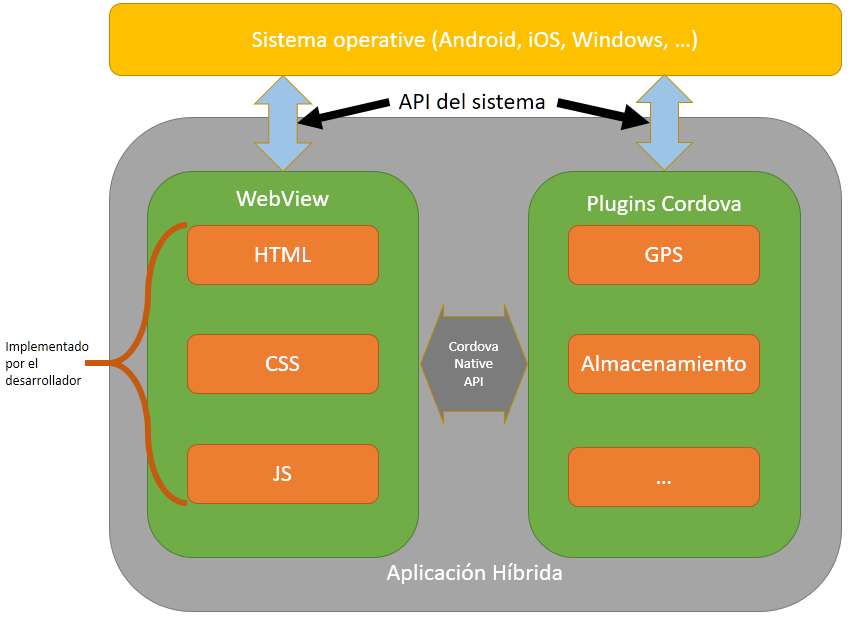
\includegraphics[width=0.8\textwidth]{Figures/ch1/cordova/diagram}
  \caption{Este diagrama muestra de forma simplificada como está compuesta una aplicación hibrida que utiliza Apache Cordova.}
\end{figure}

Cordova cuenta con una interfaz de línea de comandos (\gls{CLI}) con la podremos crear proyectos, compilarlos, ejecutarlos, \ldots. También nos servirá para añadir plugin a nuestro proyecto. El único requisito será el tener instalado en la máquina el SDK de las plataformas a las que vaya destinada nuestra aplicación.

Apache Cordova se encuentra disponible como paquete de \gls{npm}, desde donde puede ser instalada. Ver el anexo sobre \nameref{ch:ionic}.

Algunos de los frameworks que se utilizan para crear aplicaciones híbridas se colocan por ``encima'' de Cordova. Este es el caso de Ionic, framework en el que se centra este \gls{PFC}. Muchos de los comandos disponibles en Ionic \gls{CLI} no son más que envoltorios sobre el \gls{CLI} de Cordova, así como también ocurre con Ionic Native, que se coloca sobre los plugin de Cordova.

\chapter{Ionic}\label{ch:ionic}
Al tratarse de un paquete nodeJS, Ionic puede ser instalado usando \gls{npm} de una manera muy sencilla. A continuación detallaremos los pasos a seguir, asumiendo que en la máquina en la que estamos trabajando se encuentra instalado nodeJS y npm (ver anexo).
\begin{itemize}
  \item En primer lugar instalaremos Cordova, usando también para ello \gls{npm}. Para ello ejecutaremos el siguiente comando.
  \begin{lstlisting}[language=bash]
    # npm install -g cordova
  \end{lstlisting}
  El proceso puede tardar unos minutos ya que tendrá que instalar varias dependencias.
  \item Una vez instalado Cordoba, procedemos a la instalación de ionic.
  \begin{lstlisting}[language=bash]
    # npm install -g ionic
  \end{lstlisting}
\end{itemize}

\notebox{Existen dos maneras de instalar paquetes con \gls{npm}, de manera global o de manera local. Si queremos utilizar el paquete como una herramienta vía línea de comandos, debemos instalarla de manera global; en cambio, si queremos que el paquete sea una dependencia del modulo que estamos programando, debemos instalarlo de manera local. La opción \emph{--global/-g} indica a \gls{npm} que el paquete debe ser instalado de manera global ya que por defecto lo instalará de manera local.}

Para probar que se ha instalado de manera correcta, probaremos crearemos un nuevo proyecto y probaremos que funciona.
\begin{itemize}
  \item Dentro de nuestro área de trabajo, crearemos un nuevo proyecto utilizando para ello el comando \emph{ionic start} seguido del nombre de nuestro proyecto.
  \begin{lstlisting}[language=bash]
    # ionic start --v2
  \end{lstlisting}
  \item El anterior comando creará un nuevo directorio con el mismo nombre del proyecto. Dentro de este directorio descargará una templete por defecto, por lo que dentro encontraremos diferentes ficheros y directorios:
  \begin{figure}[H]
\centering
    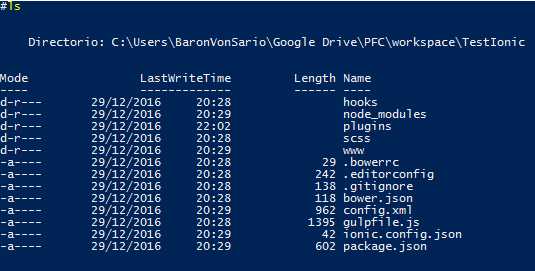
\includegraphics[width=0.8\textwidth]{Figures/anexo/anexoI/ionic/ionic_start}
    \caption{Estructura de archivos que sirve como base para empezar un nuevo proyecto con ionic. Han sido generados utilizando el comando \emph{ionic start}.}
  \end{figure}
  \item Podemos hacer que ionic ponga en marcha un servidor de desarrollo para poder acceder a la aplicación a través de un browser. Solo tenemos que ejecutar el comando \emph{ionic serve} dentro del directorio anterior. Aparecerá un mensaje indicando que el servidor está levantado además de cierta información como la url para acceder a la aplicación, los ficheros que está sirviendo o los comandos para realizar ciertas acciones.
  \begin{figure}[H]
\centering
    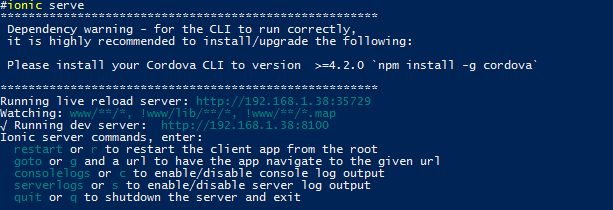
\includegraphics[width=0.8\textwidth]{Figures/anexo/anexoI/ionic/ionic_serve}
    \caption{Vemos como el servidor de la aplicación ionic está en marcha.}
  \end{figure}
  \item Si abrimos nuestro navegador y accedemos a la url que indica el servidor (por defecto será la IP de la máquina y el puerto 8100), veremos la aplicación servida, que no es más que el template descargado anteriormente:
  \begin{figure}[H]
\centering
    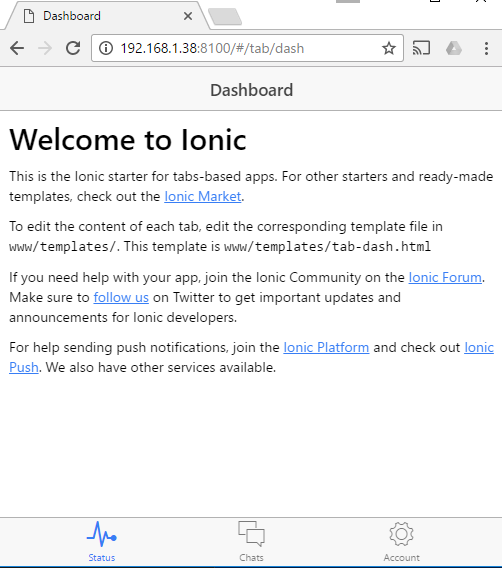
\includegraphics[width=0.8\textwidth]{Figures/anexo/anexoI/ionic/its_alive}
    \caption{La aplicación vista desde un navegador.}
  \end{figure}
\end{itemize}


\clearpage
\chapter{Prácticas} \label{ch:practices}

Una máxima en el mundo de la programación es: \emph{"La mejor forma de aprender a programar es programando"}. En este capítulo se van a proponer una serie de prácticas con los que poder ver Ionic en acción. Para la realización de estas aplicaciones, daremos por sentado que se dispone de un ordenador con Ionic2 instalado (ver anexo \nameref{ch:ionic}) y un editor de código, en nuestro caso utilizaremos \nameref{ch:atom}. Se recomienda crear un nuevo directorio que sirva como área de trabajo en el que guardaremos los proyectos.

Como se suele hacer en cualquier lenguaje de programación, comenzaremos programando un \emph{Hello World!}, esto es, una aplicación sencilla que lo único que haga sea imprimir el mensaje ``Hello World!'' en el dispositivo de salida. Esta práctica servirá de toma de contacto con la estructura de las aplicaciones construidas con Ionic. A continuación veremos como depurar nuestro desarrollo utilizando un emulador o directamente sobre un dispositivo real y como construir nuestra aplicación. Con esta base, continuaremos viendo aspecto más específico de sobre la tecnología, como el \emph{Data Binding}, los servicios, las animaciones, el uso de la \gls{API} del sistema, \ldots a través de tres prácticas es las que programaremos: un \textbf{Cronómetro} \ref{sec:crono}, un \textbf{Paisaje} \ref{sec:paisaje} y una aplicación que gestione \textbf{Recordatorios asociados a una localización} \ref{sec:recordatorios}.

Se dará por supuesto que el lector de este documento cuenta con unos conocimientos básicos de los lenguajes JavaScript, \gls{HTML} y \gls{CSS}, por lo que no se profundizará en conceptos referentes a estas tecnologías si no es estrictamente necesario.

\clearpage
\section{Hola Mundo!!!} \label{sec:hello}

El \emph{Hola Mundo} (o \emph{Hello World}) es la primera aplicación que típicamente se programa a la hora de aprender una nueva tecnología. Su funcionamiento es sencillo, imprimir por pantalla (o por el dispositivo de salida correspondiente) el saludo que da nombre a la aplicación. Con esta práctica se abordará la creación de un nuevo proyecto. También se creará una pequeña página para la que trabajaremos sobre el código \gls{HTML} de la aplicación. Veremos como probar la aplicación usando el navegador (Chrome en nuestro caso) de la máquina de desarrollo que utilizamos para desarrollar. Por último, haremos una primera aproximación a la característica de \emph{Data Binding} de Angular uniendo dos elementos del \gls{HTML} que aparecerán por pantalla.

Para crear nuestro primer proyecto, abrimos el PowerShell de Windows (o la consola de comandos tradicional, según disponibilidad y gustos personales) y nos dirigimos a nuestro directorio de trabajo. Aquí se creará el directorio que contendrá nuestro proyecto. En este caso queremos un proyecto en blanco, usando la plantilla \emph{blank}, para ello ejecutaremos el siguiente comando:

\begin{lstlisting}[language=bash]
  # ionic start HelloWorld blank --v2
\end{lstlisting}

Esto creará un directorio llamado HelloWorld dentro del cual veremos el proyecto sobre el cual vamos a trabajar.

\notebox{Con la opción \emph{--v2} indicamos que el queremos usar la versión de ionic para el nuevo proyecto.}

\begin{figure}[H]
\centering
  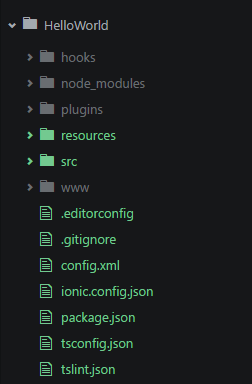
\includegraphics[height=0.4\textheight,keepaspectratio]{Figures/ch2/HelloWorld/atom_project_structure}
  \caption{Estructura del proyecto \emph{Hello World} al crearlo visto en Atom.}
\end{figure}

Podemos ejecutar la aplicación tal cual se encuentra en este momento y comprobar que funciona correctamente. Para esto, utilizando Ionic CLI, podremos ejecutar la aplicación sobre un servidor el cual servirá de servidor local para nuestra aplicación permitiéndonos acceder a ella a través de un navegador web:

\begin{lstlisting}[language=bash]
  # ionic serve
\end{lstlisting}

Tras unos segundos, nos aparecerá un mensaje indicando la \gls{URL} en la cual se encuentra disponible la aplicación. Por lo general, cuando el servidor termina de arrancar, se abrirá el navegador configurado por defecto en nuestro sistema apuntando directamente a la dirreción anterior. De no ser así, copiamos la \gls{URL} y la abrimos manualmente.
Vemos la página que por defecto viene con la plantilla utilizada.

\begin{figure}[H]
\centering
  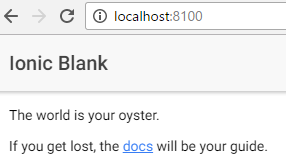
\includegraphics[width=0.4\textwidth,keepaspectratio]{Figures/ch2/HelloWorld/ionic_blank}
  \caption{Así es como se ve el template \emph{blank} al ejecutarse.}
\end{figure}

Vamos a editar la aplicación para que tenga el comportamiento antes indicado, es decir, que en nuestro caso es mostrar por pantalla el texto "Hello World!". Abrimos con el editor que vayamos a usar el fichero \emph{./src/pages/home/home.html}. Dentro de este fichero se encuentra el código de la página que acabamos de ver en el navegador.

\begin{figure}[H]
\centering
  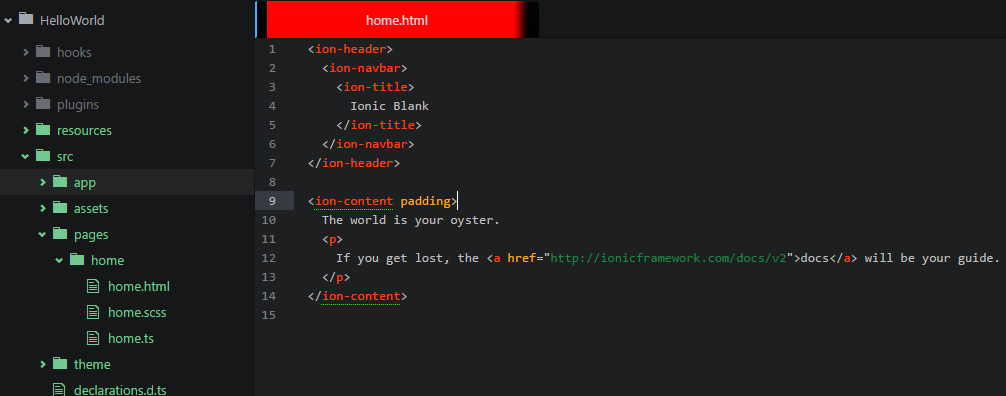
\includegraphics[width=\textwidth,keepaspectratio]{Figures/ch2/HelloWorld/home_ionic_blank}
  \caption{Página principal del template \emph{blank}.}
\end{figure}

\tipbox{Si utilizamos un editor un poco avanzado, nos ofrecerá la posibilidad de abrir un directorio de trabajo entero, pudiendo ver la estructura de ficheros de la aplicación y navegar fácilmente entre ellos.}

Podemos apreciar que la página dispone de una cabecera definida por el tag \emph{<ion-header>} y el cuerpo de la página definido por el tag \emph{<ion-content padding>}. Modificaremos el código de la siguiente manera:

\begin{lstlisting}[style=htmlcssjs,frame=tlrb,xleftmargin={0.2cm}]
  <ion-header>
    <ion-navbar>
      <ion-title>
        Hello App
      </ion-title>
    </ion-navbar>
  </ion-header>

  <ion-content padding>
    <p>HELLO WORLD!!!</p>
  </ion-content>
\end{lstlisting}

Una vez guardado el cambio, veremos en la ventana del PowerShell en la que hemos arrancada el servidor de Ionic que la aplicación se ha compilado de nuevo, y la propia página en el navegador se ha refrescado mostrando los cambios.

\begin{figure}[H]
\centering
  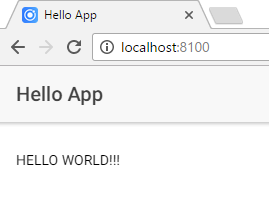
\includegraphics[width=0.4\textwidth,keepaspectratio]{Figures/ch2/HelloWorld/hello_world_1}
  \caption{Podemos ver nuestro Hello World en el navegador por primera vez.}
\end{figure}

Vamos a ir un poco más allá con nuestra aplicación. Para ello vamos a utilizar una de las características que nos ofrece Angular, el \emph{Data Binding}. Abrimos de nuevo el fichero \emph{home.html} y modificamos el cuerpo de la siguiente manera:

\begin{lstlisting}[style=htmlcssjs,frame=tlrb,xleftmargin={0.2cm}]
<ion-content padding>
  <ion-list>
    <ion-item>
      <ion-label color="primary" >My name is </ion-label>
      <ion-input [(ngModel)]="name" placeholder="your name" ></ion-input>
    </ion-item>
    <ion-item>
      <h1>Hello {{ name }}, nice to meet you.</h1>
    </ion-item>
  </ion-list>
</ion-content>
\end{lstlisting}

Con esta modificación hemos introducido un cuadro de texto, \emph{<ion-input>}, en el que podremos escribir nuestro nombre. También hemos cambiado el saludo, haciendo que este sea ``personalizado'' utilizando el valor introducido en \emph{\{\{ name \}\}}. Esto se consigue gracias a la potencia del \emph{Data Binding}. Si volvemos a ver nuestro input, vemos que uno de sus atributos es \textbf{[(ngModel)]}. Este atributo es una directiva de Angular que vincula un campo, el input en nuestro caso, con una propiedad del componente al que pertenece. Así, al declarar la directiva \emph{[(ngModel)]="name"}, hemos hecho que se cree una propiedad dentro del componente (si no la hemos creado manualmente editando el componente) y que su valor esté vinculado al del input. Ya solo nos queda utilizar este valor donde nos interesa utilizando la expresión \emph{\{\{ name \}\}}. Angular también se encarga de renderizar el valor cuando este cambia, por lo que a medida que vayamos escribiendo nuestro nombre, irá actualizándose la vista.

\begin{figure}[H]
\centering
    \centering
        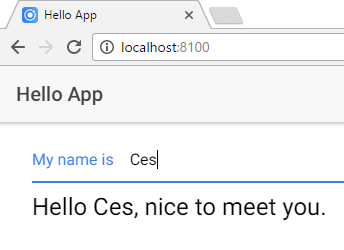
\includegraphics[width=0.3\textwidth]{Figures/ch2/HelloWorld/dyn_hello_world_1}
        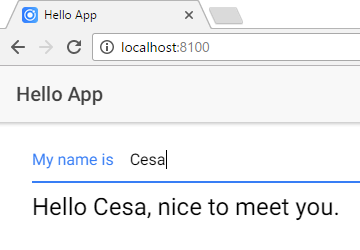
\includegraphics[width=0.3\textwidth]{Figures/ch2/HelloWorld/dyn_hello_world_2}
        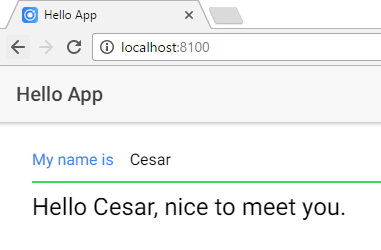
\includegraphics[width=0.3\textwidth]{Figures/ch2/HelloWorld/dyn_hello_world_3}
    \caption{Nuestra aplicación ahora nos ofrece un saludo dedicado.}
\end{figure}

\clearpage
\section{Construir y emular}

Antes de continuar con las siguientes aplicaciones, y ya que tenemos lista nuestro primer desarrollo listo para ser usado, vamos ver como podemos  ejecutarlo en un emulador y en un terminal Android real, además de poder depurar el código desde el navegador Chrome como si de una página web se tratase. De esta forma podremos ver probar la aplicación sobre un terminal real de manera fácil y rápida.

Este método no tiene porque sustituir al servidor de desarrollo local que ejecutamos con \emph{ionic serve}. Este servidor se caracteriza por ser más rápido a la hora de testear pequeños cambios, en especial si estos afectan al diseño, y sobrecarga menos la máquina en la que lo ejecutemos que lo que lo hace un emulador. Aún así, resulta evidente la necesidad de probar las aplicaciones en los terminales objetivo. Una limitación muy importante que tiene ejecutar la aplicación sobre él servidor de desarrollo es la imposibilidad de emular las \glspl{API} de los dispositivos, por lo que si queremos hacer pruebas con los sensores, por ejemplo, el \gls{GPS}, necesitaremos utilizar un emulador o un dispositivo real. Por lo general, ambas formas son usadas a la hora de desarrollar la aplicación eligiendo una u otra según el cambio que queramos probar.

Por último tendremos que generar un ejecutable válido y reconocible por el sistema para poder distribuir nuestra aplicación. Explicaremos como hacer esto generando una \gls{APK} con la que poder instalar la aplicación en terminales Android.

Nos vamos a centrar en terminales con sistema operativo Android, debido a su popularidad, a que los recursos software necesarios son gratuitos y a que no requiere de un sistema operativo especial para poder desarrollar en él. Aún así, lo explicado en este capitulo es valido para otras plataformas siempre y cuando dispongamos de los recursos necesarios.

Antes de continuar, debemos asegurarnos de que tenemos instalado en nuestra máquina la suite de Android. Podemos ver una explicación de como instalar este software necesario en el anexo \nameref{ch:androidTools}. Aunque todas la acciones que veamos a continuación las hagamos a través de Ionic CLI, este necesita usar las herramientas que proporciona \emph{Google} para generar una aplicación nativa, que es la que realmente se ejecuta en los terminales. Además, el emulador que utilizaremos forma parte de esta suite.

\subsection{Añadir plataforma objetivo}

Lo primero que debemos hacer es añadir una plataforma objetivo a nuestro proyecto. Con esto configuramos nuestro proyecto indicando para que plataformas queremos que se generen los diferentes instaladores. En primer lugar vamos a ver que plataformas tenemos disponible en nuestro ordenador. Esto lo hacemos utilizando Ionic CLI dentro del directorio de nuestro proyecto.

\begin{figure}[H]
\centering
    \centering
        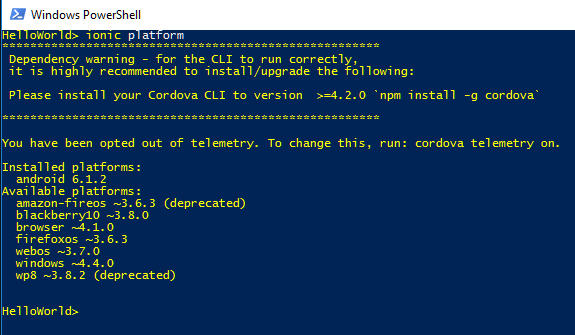
\includegraphics[width=0.8\textwidth]{Figures/ch2/BuildAndEmulate/available_platforms}
    \caption{Listado de plataformas disponibles para incluir en nuestro proyecto.}
\end{figure}

Como hemos dicho al inicio del capitulo, nos vamos a centrar en la plataforma Android, por lo que es la única que necesitamos añadir.

\begin{figure}[H]
\centering
    \centering
        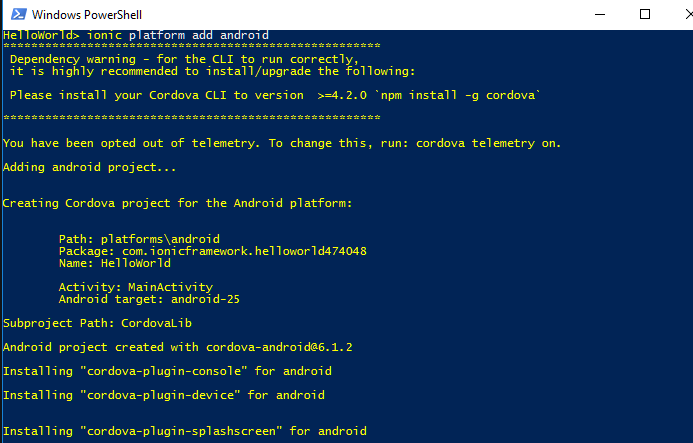
\includegraphics[width=0.8\textwidth]{Figures/ch2/BuildAndEmulate/add_android}
    \caption{Comando a ejecutar si queremos añadir la plataforma Android a la lista de plataformas objetivo de nuestra aplicación.}
\end{figure}

Con esto nuestro proyecto estaría preparado para ser ejecutado en un terminal o emulador Android, y para más tarde, generar el \gls{APK}.

\subsection{Emular aplicación}

Como se ha comentado, Ionic CLI nos permite arrancar un emulador Android en nuestra máquina de desarrollo y ejecutar sobre él la aplicación. Para ello utiliza Android Emulator, un emulador que ofrece Google como parte del \gls{SDK} de Android. Ionic se encarga, ejecutando un único comando, de compilar el proyecto, generar el instalable, arrancar el emulador e instalar en él nuestra aplicación. Un ejemplo del comando que hace todo esto es:

\begin{lstlisting}[language=bash]
  # ionic emulate android --target=Nexus5
\end{lstlisting}

Como vemos, en el comando debemos indicar sobre que plataforma queremos realizar la emulación. Como opción, podemos seleccionar que \gls{AVD} queremos utilizar, en caso de no indicarlo, Ionic CLI utilizará el primero que encuentre. Podemos encontrar más información sobre los \gls{AVD} en el anexo \nameref{ch:androidTools}, y más concretamente, en la sección \nameref{sec:AndroidEmulator}.

La ejecución de este comando iniciará una serie de tareas que podremos ir viendo aparecer en la consola. Justo antes de acabar (tarda unos segundos), se iniciará el emulador (si no estaba ya en ejecución) y a continuación, se iniciará la aplicación automáticamente en este.

\begin{figure}[H]
\centering
    \centering
        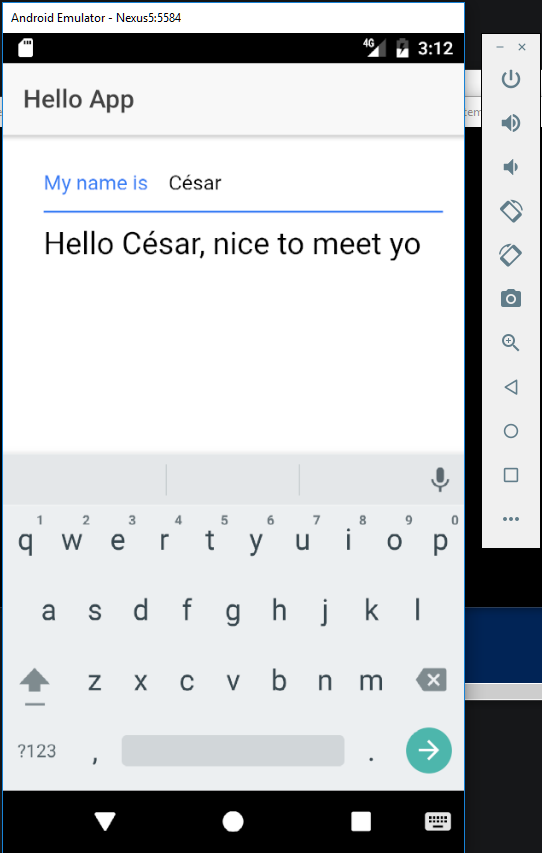
\includegraphics[width=0.4\textwidth]{Figures/ch2/BuildAndEmulate/landscape_emulator}
    \caption{Nuestra aplicación vista en el emulador.}
\end{figure}

\subsection{Depurar una aplicación que está siendo emulada}

Ya hemos dicho que durante la false de desarrollo, la mejor forma de probar y depurar nuestra aplicación es haciendo uso de la utilidad \emph{ionic serve} y de nuestro navegador favorito. Aún así, en ocasiones es necesario poder depurar la aplicación mientras se ejecuta en el emulador, por ejemplo, para probar el uso de determinados sensores, gestos sobre la pantalla que no podemos realizar en el navegador o simplemente comprobar que la aplicación se ve como debe en un terminal similar al emulado.

Para esto vamos a utilizar el navegador Chrome, que nos permite acceder a las aplicaciones que se ejecuten en el emulador o terminal conectado que usen tecnología web. Aunque aquí nos centramos en aplicaciones híbridas, podemos usar también este mismo método para aplicaciones que se estén ejecutando en el navegador del dispositivo. Vamos a emular la aplicación del mismo modo que hicimos anteriormente:

\begin{lstlisting}[language=bash]
  # ionic emulate android --livereload --target=Nexus5
\end{lstlisting}

Añadiendo \emph{--livereload} conseguimos algunas de las facilidades que tenemos al utilizar \emph{ionic serve}:

\begin{enumerate}
  \item Ver los cambios realizado en el código de manera inmediata sin necesidad de tener que volver a lanzar el comando para que vuelva a compilar la aplicación y la vuelva a ejecutar.
  \item Poder depurar el código sin que este esté compilado.
\end{enumerate}

\warningbox{En el momento de escribir este documento, la opción \emph{--livereload} se encuentra en fase \emph{beta}, por lo que puede no funcionar correctamente. De ser así, nos veremos obligados a usar el método manual y recompilar la aplicación cada vez que efectuemos un cambio.}

Una vez que la aplicación se esté ejecutando, iniciamos el \emph{Chrome} y abrimos la consola para desarrolladores (desde las opciones de Chrome > Más herramientas > Herramientas de desarrolladores, o pulsando F12, o pulsando ctrl + shift + I). Dentro de la consola, en opciones > \emph{More tools} seleccionamos \emph{Remote Devices}.

\begin{figure}[H]
\centering
    \centering
        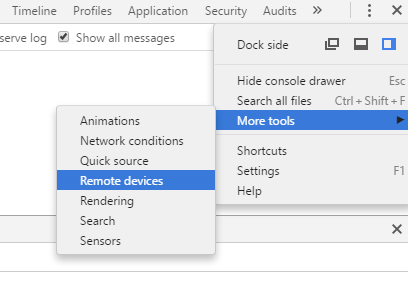
\includegraphics{Figures/ch2/BuildAndEmulate/how_open_remote_devices}
    \caption{Opción para abrir la ventana de dispositivos remotos.}
\end{figure}

Esto nos abrirá una ventana dentro de la consola donde aparecerán todos los dispositivos que tengamos conectados (emuladores, terminales conectados al PC, incluso los Chromecast si disponemos de alguno en nuestra red). En esta lista de dispositivos encontraremos nuestro emulador, en él, aparecerá nuestra aplicación, la cual podremos \emph{Inspeccionar}.

\begin{figure}[H]
\centering
    \centering
        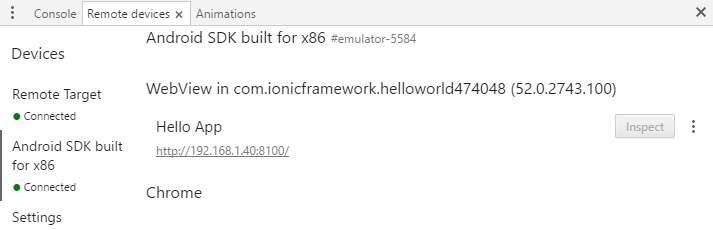
\includegraphics[width=0.8\textwidth]{Figures/ch2/BuildAndEmulate/remote_devices_list}
    \caption{Lista de dispositivos disponibles para depurar. Entre ellos se encuentra nuestro emulador con nuestra aplicación híbrida abierta.}
\end{figure}

Si seleccionamos la opción inspeccionar, se nos abrirá una ventana del navegador en la que veremos lo mismo que se esta viendo en esos momentos en el emulador. Podremos ver el detalle de los elementos del \gls{HTML} de la misma manera que si fuera una página web corriente abierta directamente en el navegador. Además, podremos controlar la aplicación desde el navegador, así, cualquier acción que llevemos a cabo, como pulsar algún elemento, escribir, arrastar con el botón del ratón pulsado, \ldots  se verá reflejado también en el navegador.

Podremos acceder a los ficheros \emph{.ts} y poner puntos de ruptura donde nos interese detener la ejecución del código. Como se comentaba anteriormente, esta posibilidad solo se da con la opción \emph{--livereload}. De no ser así, tendremos que buscar el trozo de código que nos interesa en el fichero ya compilado.

\begin{figure}[H]
\centering
    \centering
        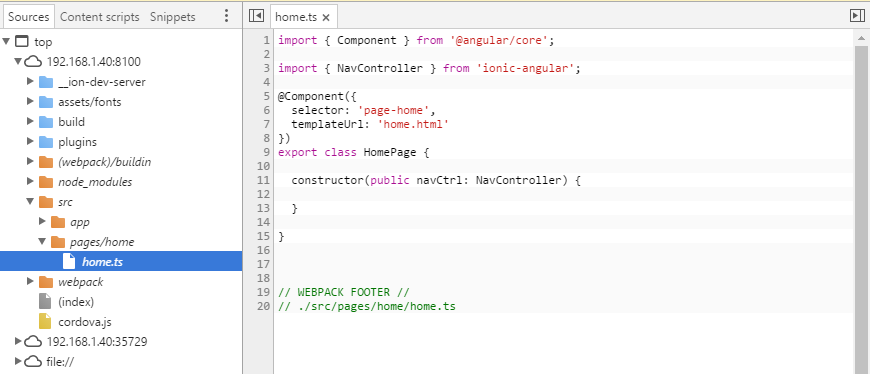
\includegraphics[width=\textwidth]{Figures/ch2/BuildAndEmulate/livereload_code_dev_tool}
        \hfill \break
        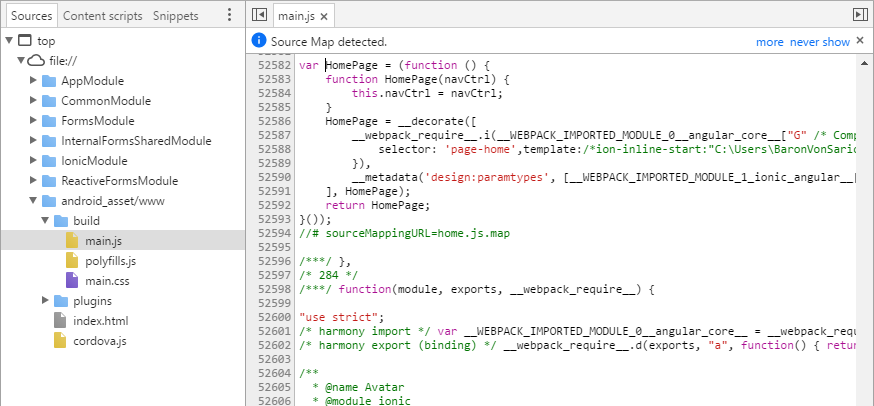
\includegraphics[width=\textwidth]{Figures/ch2/BuildAndEmulate/nolivereload_code_dev_tool}
    \caption{Diferencia entre como se ve el código sin compilar, emulado con la opción \emph{--livereload} (arriba), y el código compilado (abajo).}
\end{figure}

Podemos probar a cambiar el código y ver como la aplicación se recarga nada más guardamos el cambio. Por ejemplo, vamos a hacer que se escriba una entrada en el log al iniciar la aplicación. Abrimos el fichero \emph{home.ts} de nuestra página y editamos el constructor de la siguiente manera:

{\begin{lstlisting}[style=htmlcssjs,frame=tlrb,xleftmargin={0.2cm}]
constructor(public navCtrl: NavController) {
    console.log("HelloWorld application is running."):
  }

\end{lstlisting}}

Una vez que la aplicación haya terminado de recargar, apenas tarda unos segundos, podremos comprobar que el cambio en efecto se ha efectuado y ver en la consola el mensaje anterior.

\begin{figure}[H]
\centering
    \centering
        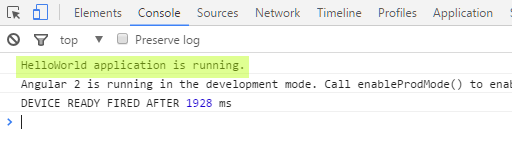
\includegraphics[width=0.8\textwidth]{Figures/ch2/BuildAndEmulate/state_log}
    \caption{La aplicación muestra por consola el mensaje de inicio.}
\end{figure}

También podremos hacer el cambio sobre el script que se está ejecutando sobre el mismo navegador y guardar el cambio utilizando la combinación ctrl + s. Este cambio solo será temporal y hasta que se vuelva a recargar el fichero JavaScript, pero será válido siempre que el flujo de ejecución pase por él. Tampoco modifica el código sobre el que estamos trabajando, ya que el cambio se guarda en la versión del script que utiliza el navegador.

\subsection{Ejecutar una aplicación en un terminal conectado} \label{subsec:runInDevice}

Si disponemos de uno o varios terminales en los que poder probar la aplicación, podemos conectarlos a nuestro ordenador y hacer que ejecute el código del mismo modo que ocurre en el emulador teniendo también la opción de depuración desde Chrome.

En primer lugar, debemos tener el terminal conectado al ordenador, y asegurarnos de tener todos los drivers instalados. Además, debemos de habilitar el modo \emph{debug} vía \gls{USB} en el móvil y autenticar nuestro PC en el móvil. En la web de desarrolladores de Google nos explican como poder hacer esto \emph{https://developers.google.com/web/tools/chrome-devtools/remote-debugging/}.

Cuando tengamos nuestro terminal listo, llegará el momento de ver nuestra aplicación en él. Como podremos imaginar, esto se consigue utilizando Ionic CLI:

\begin{lstlisting}[language=bash]
  # ionic run android --livereload
\end{lstlisting}

Y listo. Si todo va bien, al cabo de unos segundos debería aparecer nuestra aplicación en el terminal.

Al igual que ocurría con el emulador, podremos depurar nuestra aplicación utilizando el navegador Chrome, siguiendo los mismos pasos explicados anteriormente, pero seleccionando nuestro terminal en la lista de dispositivos.

\begin{figure}[H]
\centering
    \centering
        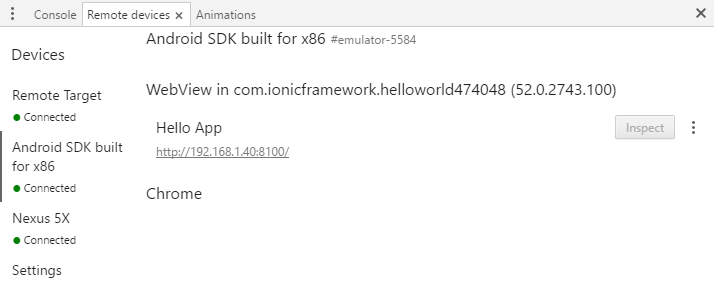
\includegraphics[width=0.8\textwidth]{Figures/ch2/BuildAndEmulate/remote_devices_list_nexus5}
    \caption{El terminal Android conectado a nuestro equipo aparece listado entre los dispositivos disponibles en Chrome.}
\end{figure}

Esta operación nos dejaría la aplicación instalada en nuestro terminal, por lo que al desconectar el dispositivo del ordenador podríamos seguir usandola como si de otra aplicación se tratase (algo útil si necesitamos hacer pruebas con el \gls{GPS}).

\subsection{Generar el instalador. El APK.}

Cuando ya demos por buena nuestra aplicación, o simplemente queramos compartirla con alguien sin tener que compartir el código y haciendo que sea él quien lo compile, será el momento de generar el instalador para las diferentes plataformas. Como estamos trabajando para la plataforma Android, en nuestro caso generaremos un fichero \emph{.apk}. Este fichero podremos compartirlo con cualquier usuario de Android y podrá instalarlo en su dispositivo. También podrá ser subido a la tienda de aplicaciones de Android, \emph{Play Store}, para que pueda ser descargado por cualquier usuario. Para esto último, será necesario firmar el \gls{APK}.

Antes de esto, vamos a darle un último toque de personalización a nuestra aplicación. Si ya hemos ejecutado la aplicación en el terminal como se explicaba en el apartado anterior, nos habremos fijado en dos detalles. Por un lado, el icono que aparece en nuestro dispositivo representando a nuestra aplicación es el icono de Apache Cordova. Con el splash, la pantalla que aparece al iniciar la aplicación, ocurre lo mismo. Ambos son generados y configurados por defecto al añadir una nueva plataforma al proyecto.

Para poder personalizar tanto el icono como el splash, necesitamos de una imagen para cada uno de ellos en formato \emph{.png, .psd o .ai}. Ambas tendrán que tener el elemento principal de la imagen debe estar centrado, ya que Ionic recortará la imagen para ajustarla a diferentes tamaños de pantalla. En cuanto al tamaño, el icono tendrá que tener un tamaño mínimo de 192x192 píxeles y no tendrá que tener los bordes redondeados ya que este efecto lo aplica la propia plataforma. El splash, deberá medir un mínimo de 2208x2208 píxeles.

Una vez creadas las imágenes, tendremos que colocarlas dentro de nuestro proyecto en la capeta \emph{resources} con los nombres \emph{icon.png y splash.png} (o con la extensión del formato que hayamos elegido). Ejecutamos de nuevo un comando proporcionado por Ionic CLI el cual generará, a partir de nuestras imágenes, diferentes iconos y splash para los diferentes dispositivos y los dejará preparados para cuando se genere el instalador.

\begin{lstlisting}[language=bash]
  # ionic resources
\end{lstlisting}

\notebox{El comando \emph{ionic resources} dispone de dos opciones, \emph{--icon y --splash}, por si solo queremos generar uno de los dos elementos.}

Para más información, podemos consultar la documentación que proporciona Ionic en su primera versión, pero que también es aplicable para la versión 2 en  \url{http://ionicframework.com/docs/cli/icon-splashscreen.html}.

Ya con todo listo, podemos generar nuestro APK. Ejecutamos el siguiente comando:

\begin{lstlisting}[language=bash]
  # ionic build android
\end{lstlisting}

Al finalizar, aparecerá la ruta donde se encuentra el APK. Lo renombramos con un nombre que nos resulte identificable y ya podemos probar a instalarlo en cualquier dispositivo Android.

\warningbox{En caso de tener ya la aplicación instalada por otro método, por ejemplo el explicado en el punto \nameref{subsec:runInDevice}, es posible que no podamos instalar la aplicación y recibamos un error a cambio. En este caso, es mejor desinstalar la aplicación y probar de nuevo. Lo mismo puede ocurrir si intentamos la misma operación pero en orden inverso.

Esto ocurre debido a que el nombre de la aplicación que usa Android internamente para identificarla es el mismo, pero la fuente de instalación son diferentes, por lo que pueden entrar en conflicto.}

\clearpage
\section{Cronómetro} \label{sec:crono}

Con el \emph{Hello World!!!} hemos visto como crear nuestro proyecto y una de las características más potentes de Angular, el \emph{Data Binding}. Ahora vamos a dar un pasito más y vamos crear una aplicación que sirva como cronómetro. Para ello, además de usar el \emph{Data Binding}, que por otro lado va a estar presente en la mayoría de desarrollos, veremos como modificar datos desde la lógica del componente y que estos cambias se vean reflejados en la vista. Además introduciremos algunas directivas de Angular, como es \textbf{*ngFor}, que utilizaremos para recorrer listas que formen parte del componente desde la propia plantilla

El primer paso, como no podría ser de otra manera, será crear un nuevo proyecto en blanco dentro de nuestro directorio de trabajo, de la misma forma que vimos en el capítulo anterior sobre el \nameref{sec:hello}:

\begin{lstlisting}[language=bash]
  # ionic start Chronometer blank --v2
\end{lstlisting}

En primer lugar vamos a hacer un cronómetro que tenga como unidad de medida mínima el segundo. También añadiremos dos botones, uno que actuará como Start/Pause para iniciar y detener el cronómetro, y otro que actuará como Stop, y que pondrá a cero de nuevo el cronómetro.

En la página web oficial de Ionic podemos encontrar una sección dedicada a los componentes\footnote{\url{https://ionicframework.com/docs/v2/components}} que nos ofrece el framework. Aquí podremos encontrar el componente que se utiliza para poder crear un botón, y las opciones que permite, como por ejemplo las dimensiones. También podremos encontrar una sección, llamada \emph{Ionicons}\footnote{\url{https://ionicframework.com/docs/v2/ionicons/}}, en la que encontraremos iconos que ofrece el propio framework. Lo interesante de estos iconos es que se adaptan según la plataforma es la que se ejecuta la aplicación, haciendo que el \emph{Look and Feel} de esta sea coherente con la plataforma en cuestión.

\begin{figure}[H]
\centering
  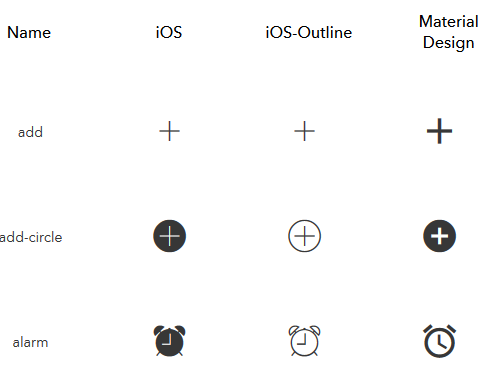
\includegraphics{Figures/ch2/Chronometer/ionicons}
  \caption{Una pequena parte de los iconos que ofrece Ionicons. Podemos ver la diferencia que existen entre ambas plataformas.}
\end{figure}

Empezaremos editando el fichero \emph{home.html} y creando un cronómetro con los elementos que queramos que lo compongan. De momento usaremos valores fijos, sin añadir ningún tipo de lógica, pudiendo así ver como queda el diseño escogido. Aquí cada cual puede utilizar el diseño que quiera, en mi caso, he optado por uno sencillo:

\begin{lstlisting}[style=htmlcssjs,frame=tlrb,xleftmargin={0.2cm}]
  <ion-content padding>
    <p style="text-align: center; font-size: -webkit-xxx-large;" >
      00:00:00
    </p>

    <ion-row>
      <ion-col>
        <button ion-button  color="secondary" full large >
          <ion-icon name="play" ></ion-icon>
          Start
        </button>
      </ion-col>
    </ion-row>

    <ion-row>
      <ion-col>
        <button ion-button color="danger" full large >
          <ion-icon name="square" ></ion-icon>
          Stop
        </button>
      </ion-col>
    </ion-row>
  </ion-content>
\end{lstlisting}

Con este diseño, nuestra página se vera tal que así:

\begin{figure}[H]
\centering
  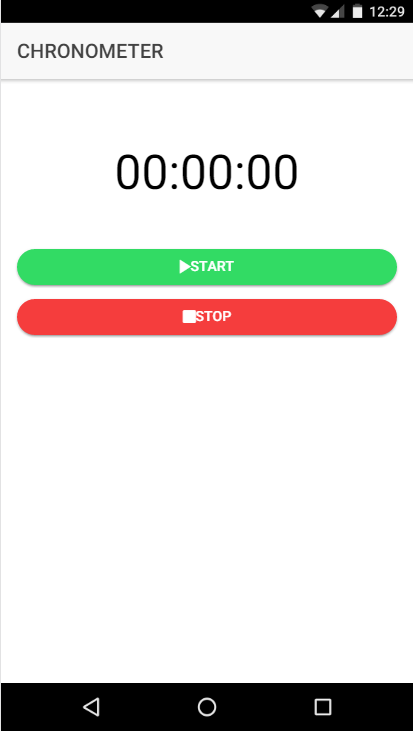
\includegraphics[width=0.4\textwidth]{Figures/ch2/Chronometer/1}
  \caption{Esto sí que es un cronómetro sencillo.}
\end{figure}

\notebox{El navegador Chrome nos da la opción de simular la vista de un dispositivo móvil y poder así comprobar como se ve nuestra aplicación limitada a diferentes tamaños de pantalla. Para ello, tendremos que abrir la herramienta para desarrolladores pulsando F12, y activamos \emph{Device Toolbar} con el botón 
\includegraphics{Figures/ch2/Chronometer/toggle_device_toolbar} o pulsando Ctrl+Shift+M. Esto nos abrirá una barra superior en la que podremos elegir entre diferentes modelos de dispositivos o definir el tamaño de la pantalla en píxeles manualmente.
Aunque por lo general suele ser un comportamiento cercano a la realidad, en ocasiones el resultado visto aquí y el que después vemos en la realidad puede variar en lo referente a dimensiones y posiciones de algunos elementos.}

Siguiente paso, añadir lógica a nuestra aplicación, para ello vamos a editar el fichero \emph{home.component.ts}. En este fichero \emph{TypeScript} encontramos la clase \emph{HomePage}, la cual esta precedida por el decorador \emph{@Component} de Angular. Esto quiere decir que esta clase se trata de un componente de Angular. Es este decorador se definirán los metadatos del componente, en este caso, se han definido dos de ellos: el \emph{template} y el \emph{selector}, los cuales indican el código o fichero \gls{HTML} que define el aspecto visual del componente en el caso del \emph{template} y el nombre del tag \gls{HTML} que representa este controlador en el caso del \emph{selector}. Gracias al \emph{Data Binding}, las propiedades y métodos que definamos dentro de este controlador, serán accesibles desde el código \gls{HTML} si es necesario. En primer lugar, vamos a pensar que variables precisamos para la implementación del cronómetro:

\begin{itemize}
  \item Un \emph{flag} que nos indique si el cronómetro está o no en marcha.
  \item Un contador para que almacene los segundos desde la puesta en marcha.
  \item Para que el botón Start/Pause cambie según el estado, necesitaremos hacerlo usando dos variables:
  \begin{itemize}
    \item Una cadena de texto que almacene la el texto que aparece en el botón: \emph{Start} o \emph{Pause}
    \item Una cadena que indique que icono usar en el botón.
  \end{itemize}
\end{itemize}

Todas estás variables serán inicializadas en el constructor. Para cumplir con esto requisitos utilizamos el siguiente código:

\begin{lstlisting}[style=htmlcssjs,frame=tlrb,xleftmargin={0.2cm}]
  _is_running:boolean;
  seconds:number;
  start_pause_label: string;
  start_pause_icon: string;

  constructor() {
    this.is_running = false;
    this.seconds = 0;
  };
\end{lstlisting}

\tipbox{Es una práctica recomendable que los nombres de las propiedades, de las funciones, de las clases, \ldots sean autodescriptivos, ya estemos trabajando con TypeScript como con cualquier otro lenguaje.}

No hemos inicializado ni \emph{start\_pause\_label} ni \emph{start\_pause\_icon} por la siguiente razón, estas variables están ligadas al estado en que se encuentra el cronómetro, es decir a \emph{\_is\_running}. Para asegurarnos que estos valores cambian al cambiar \emph{\_is\_running}, vamos a personalizar el \emph{getter} y el \emph{setter}\footnote{\url{https://www.typescriptlang.org/docs/handbook/classes.html#accessors}} de esta propiedad, esta es la razón por la que se ha prefijado el nombre de la propiedad con una barra baja (\_) evitando así el conflicto que se produciría con los nombres. Los métodos quedarían de la siguiente manera:

\begin{lstlisting}[style=htmlcssjs,frame=tlrb,xleftmargin={0.2cm}]
  public get is_running() {
    return this._is_running;
  };

  public set is_running(new_state) {
    this._is_running = new_state;
    this.start_pause_label = this.is_running ? "Pause" : "Start";
    this.start_pause_icon = this.is_running ? "pause" : "play";
  };
\end{lstlisting}

Cada vez que se haga una consulta a la propiedad \emph{is\_running}, se ejecutará la primera función, y cuando se asigne un valor (como ocurre en el constructor al ejecutar \emph{this.is\_running = false;}), se ejecutará la segunda función, la cual asigna el nuevo valor a \emph{is\_running}, y según sea este, a \emph{start\_pause\_label} y \emph{start\_pause\_icon}.

Llega el momento de implementar los métodos, para lo cual vamos a realizar un ejercicio anterior a la codificación similar al que hicimos con las propiedades. Los métodos que considero necesarios son para conseguir hacer funcionar nuestro cronómetro son:

\begin{itemize}
  \item Un método que sirva para cambiar el estado del cronómetro y que funcione si fuera un interruptor.
  \item Otro que sirva para detener el cronómetro y ponerlo a 0 el contador.
  \item Un último método que aumente en 1 los segundos si cronómetro está en marcha.
\end{itemize}

Al implementar estos métodos, nos quedará el componente de la siguiente manera:

\begin{lstlisting}[style=htmlcssjs,frame=tlrb,xleftmargin={0.2cm}]
  export class HomePage {
    private _is_running:boolean;
    seconds:number;
    start_pause_label: string;
    start_pause_icon: string;

    constructor() {
      this.is_running = false;
      this.seconds =0;

      setInterval(() => {
        this.tick();
      }, 1000);
    };

    public get is_running() {
      return this._is_running;
    };

    public set is_running(new_state) {
      this._is_running = new_state;
      this.start_pause_label = this.is_running ? "Pause" : "Start";
      this.start_pause_icon = this.is_running ? "pause" : "play";
    };

    tick(): void {
      if (this.is_running) {
        this.seconds++;
      }
    };

    toggle(): void {
      this.is_running = !this.is_running;
    };

    stop(): void {
      this.is_running = false;
      this.seconds = 0;
    };
  }
\end{lstlisting}

Para que la función \emph{tick()} tenga sentido, es necesario que se ejecute cada segundo. Vamos a usar la función \emph{setInternal()}. Esta función es nativa de JavaScript y por ello podemos hacer uso de ella desde TypeScript. La invocamos en el constructor indicando el método al que tiene que llamar y la espera entre una llamada y otra (el tiempo que se le pasa debe estar expresado en milisegundos):

\begin{lstlisting}[style=htmlcssjs,frame=tlrb,xleftmargin={0.2cm}]
  constructor() {
    // RESTO DE FUNCIÓN
    setInterval(() => {
      this.tick();
    }, 1000);
  };
\end{lstlisting}

Otra opción sería llamar a la función \emph{setInternal()} en el \emph{setter} de \emph{is\_running} y asignar el id devuelto a una variable del controlador, y así poder desactivarlo con la función \emph{clearInterval()}, la cual acepta como parámetro el ID anterior. Algo como:


\begin{lstlisting}[style=htmlcssjs,frame=tlrb,xleftmargin={0.2cm}]
  public set is_running(new_state) {
    this._is_running = new_state;
    if (this.is_running) {
      this.start_pause_label = "Pause"
      this.start_pause_icon = "pause"
      this.interval_id = setInterval(() => {
        this.tick();
      }, 1000);
    } else {
      this.start_pause_label = "Start"
      this.start_pause_icon = "play"
      clearInterval(this.interval_id);
    }
  };
\end{lstlisting}

La ventaja de esta opción es que se evita la llamada a la función \emph{tick()} cuando el cronómetro está detenido.

Con la lógica ya implementada, vamos a conectar las propiedades del componente con los elementos de la template, y para ello nos ayudaremos del famoso \emph{Data Binding}. Como nuestra template esta asignada al componente definido por la clase \textbf{HomePage}, podremos hacer uso de sus propiedades y métodos. Para hacer funcionar el cronómetro, necesitaremos:

\begin{enumerate}
  \item Por un lado modificar los valores mostrados en el \gls{HTML} para que coincidan con los definidos en el componente. Esto se hace poniendo el nombre de la variable o del método entre llaves dobles ( \{\{ NOMBRE \}\} ) en el \gls{HTML} allí donde queramos que el valor aparezca.
  \item Vincular el evento de \emph{click} sobre los botones a alguno de los métodos. Esto se consigue gracias a la directiva \textbf{(clic)} que se pone como atributo \gls{HTML} en el botón.
\end{enumerate}

El código se vería de la siguiente manera:

\begin{lstlisting}[style=htmlcssjs,frame=tlrb,xleftmargin={0.2cm}]
  <p style="text-align: center; font-size: -webkit-xxx-large;" >
    {{ seconds }}
  </p>

  <ion-row>
    <ion-col>
      <button ion-button  color="secondary" full large (click)="toggle()" >
        <ion-icon name="{{ start_pause_icon }}" ></ion-icon>
        {{ start_pause_label }}
      </button>
    </ion-col>
  </ion-row>

  <ion-row>
    <ion-col>
      <button ion-button color="danger" (click)="stop()" style="width: 100%;" >
        <ion-icon name="square" ></ion-icon>
        Stop
      </button>
    </ion-col>
  </ion-row>
\end{lstlisting}

Vemos que hemos cambiado el display donde se visualizan los segundos, el icono y el texto del boton ``Start''/``Pause'', se han añadido las directivas \emph{(clic)} para que hagan llamadas a las funciones que implementamos en nuestra clase \emph{HomePage} \ldots pero vemos que la forma de visualizar el tiempo transcurrido no es la que teníamos en mente, si no que vemos el número que utilizamos para contar los segundos desde el inicio, lo cuál no es intuitivo a la hora de leerlo.

Necesitamos por tanto, darle un formato más legible. Para esto vamos a usar otra herramienta que nos ofrece Angular, las llamadas \emph{Pipes o tuberias}.

El concepto de \emph{Pipe} es similar al que se utiliza por ejemplo en \emph{bash} o \emph{sh}, y nos permite transformar un dato, el cual se le pasa como entrada a la tubería, y obtenemos el mismo dato ya transformado. Para nuestra aplicación necesitamos que nuestros segundos, que no es más que un número que representa la cantidad de segundos desde el inicio a nivel lógico, se convierta en una cadena de texto con un formato más amigable para el usuario, \emph{0h 00m 00s}. Angular dispone de algunos \emph{Pipes} ya definidos\footnote{\url{https://angular.io/docs/ts/latest/api/#!?query=pipe}}, pero en nuestro caso, definiremos uno propio.

Empezaremos creando un nuevo fichero \emph{.ts} al que llamaremos \emph{home.pipes.ts}. Con esto conseguimos que el código quede MAS ORDENADO. Dentro de este fichero crearemos nuestra clase, la cual deberá implementar la interfaz \textbf{PipeTransform} y ser decorada con \emph{@Pipe}. Al implementar la interfaz \textbf{PipeTransform} tendremos que definir el método \textbf{transform()}. Este será el método que se ejecute cuando nuestra tubería sea usada, pasando la entrada de esta como parámetro. El decorador \emph{@Pipe} acepta el argumento \textbf{name}, el cuál nos permite asignar un identificador a nuestra tubería.

\begin{lstlisting}[style=htmlcssjs,frame=tlrb,xleftmargin={0.2cm}]
  @Pipe({name: 'time_format'})
  export class MyTimePipe implements PipeTransform {
    transform(seconds: number): string {
      var s_num = seconds % 60;
      var m_num = Math.floor((seconds % 3600) / 60);
      var h_num = Math.floor(seconds / 3600);

      var s = ('0' + s_num).slice(-2);
      var m = ('0' + m_num).slice(-2);
      var h = '' + h_num;

      return '\${h}h \${m}m \${s}s';
    }
  }
\end{lstlisting}

Ya solo nos queda utilizar esta tubería en nuestro template. Cambiamos la llamada a la variable \emph{seconds} para que pase por nuestra tubería:

\begin{lstlisting}[style=htmlcssjs,frame=tlrb,xleftmargin={0.2cm}]
  <p style="text-align: center; font-size: -webkit-xxx-large;" >
    {{ seconds | time_format }}
  </p>
\end{lstlisting}

Al utilizar esta tubería, conseguimos que el contador de segundos siga siendo un número, lo que facilita su uso en otras partes del código. También tenemos disponible un método sencillo y reusable para convertir segundos a un formato entendible para el usuario y que volveremos a usar en el siguiente apartado.

\subsection{Cronómetro con contador de vuelta}

Vamos a añadir una función extra a nuestro cronómetro, un contador de vueltas. Este contador nos permitirá guardar el registro en un momento dado sin detener el cronómetro. Estos registros que se vayan guardando aparecerán en una lista debajo de la botonera, la cuál también modificaremos para añadir dos nuevos botones.

\begin{figure}[H]
\centering
  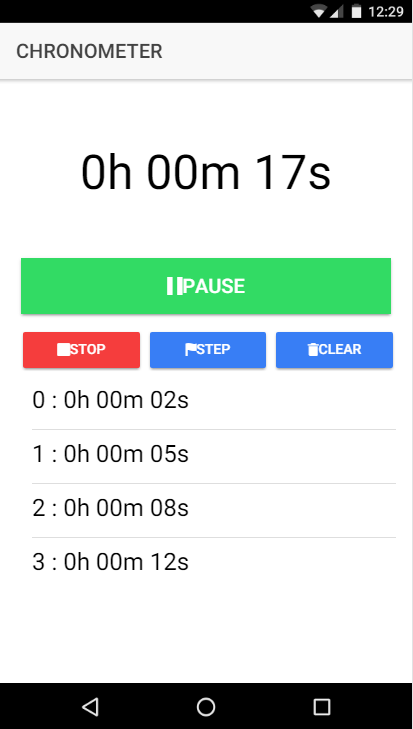
\includegraphics[width=0.4\textwidth]{Figures/ch2/Chronometer/chronometer_v2}
  \caption{En esta nueva versión hemos añadido dos nuevos botones además de una lista con los tiempos guardados.}
\end{figure}

Veamos a continuación las modificaciones hechas a nuestro \gls{HTML} para introducir los nuevos botones y la lista.

\begin{lstlisting}[style=htmlcssjs,frame=tlrb,xleftmargin={0.2cm}]
  <ion-content padding>
  <p style="text-align: center; font-size: -webkit-xxx-large;" >
    {{ seconds | time_format }}
  </p>

  <ion-row>
    <ion-col>
      <button ion-button  color="secondary" full large (click)="toggle()" >
        <ion-icon name="{{ start_pause_icon }}" ></ion-icon>
        {{ start_pause_label }}
      </button>
    </ion-col>
  </ion-row>

  <ion-row>
    <ion-col>
      <button ion-button color="danger" (click)="stop()" style="width: 100%;" >
        <ion-icon name="square" ></ion-icon>
        Stop
      </button>
    </ion-col>
    <ion-col>
      <button ion-button (click)="step()" style="width: 100%;" >
        <ion-icon name="flag" ></ion-icon>
        Step
      </button>
    </ion-col>
    <ion-col>
      <button ion-button (click)="clear()" style="width: 100%;" >
        <ion-icon name="trash" ></ion-icon>
        Clear
      </button>
    </ion-col>
  </ion-row>
  <ion-list>
    <ion-item  *ngFor="let step of step_list; let i=index" >
      <h1>{{ i }} : {{ step  | time_format }}</h1>
    </ion-item>
  </ion-list>
  </ion-content>
\end{lstlisting}

Los botones no tienen más misterio que los que se explicaron antes, cambiando la función a la que llaman, las cuales implementaremos más adelante.

Sí que nos encontramos dos componente nuevos de Ionic, \textbf{ion-list} y \textbf{ion-item}. Como bien se puede intuir por sus nombre, estos componentes sirven para crear listas y elementos dentro de ellas. Dentro del componente ion-item también vemos el atributo \textbf{*ngFor}. Este atributo se trata de una directiva de Angular que nos permite recorrer una lista, que definiremos en el componente, y por cada iteración renderizará el elemento que contiene la directiva, en este caso, el ion-item. En cada iteración sobre la lista, el valor recuperado se almacena en una variable (let step of step\_list) a la que se puede acceder del mismo modo que si se tratara de una propiedad del componente, pudiendo tratarla con nuestra tubería personalizada de igual manera que hacíamos con los segundos. Como opción, podemos recuperar el índice, que representa la posición que ocupa el elemento en la lista, y asignarlo a una variable (let i=index) que como no, también podemos usar como la anterior.

En lo que respecta a la lógica, necesitaremos implementar las dos funciones a las que se llamarán desde los nuevos botones, y una lista que almacene los registros que vayamos guardando. Desde una de las funciones haremos que se añada a la lista el tiempo actual, desde la otra limpiaremos la lista. Como ocurre con el resto de propiedades, cada vez que modifiquemos la lista, se actualizará la vista de la misma manera que pasaba con los segundos, sin importar que la variable se encuentre dentro de la directiva *ngFor.

\begin{lstlisting}[style=htmlcssjs,frame=tlrb,xleftmargin={0.2cm}]
  export class HomePage {
    // RESTO DE VARIABLES
    step_list: number[];

    // RESTO DE FUNCIONES
    step(): void {
      if (this.is_running) {
        this.step_list.push(this.seconds);
      }
    }

    clear(): void {
      this.step_list = [];
    }
  }
\end{lstlisting}

Estas nuevas funciones serán ejecutadas cada vez que pulsemos sobre los correspondientes botones ya que como vimos antes, han sido asignados utilizando la directiva \textbf{(click)}.

\clearpage
\section{Paisaje} \label{sec:paisaje}

En esta práctica vamos a centrarnos en el uso del \gls{CSS} y de las animaciones. Antes de nada, haremos una pequeña introducción a qué es y como funciona \gls{CSS} y como podemos trabajar con el en Ionic2.

\gls{CSS} es un leguaje utilizado para definir la presentación de un documento estructurado escrito en un lenguaje de marcado. Esto, cuando trabajamos con tecnología Web, se refiere al estilo a aplicar nuestra página, la cual está escrita en \gls{HTML}, que actúa como lenguaje de marcado. Así, mientras que nuestro código \gls{HTML} contiene la información, el código \gls{CSS} define la presentación. Con esta separación entre información y presentación se consigue un mayor control y modularidad.

La última especificación de \gls{CSS} es la número 3, la que se conoce como \gls{CSS3}.

Una de las características mas útiles y que más han evolucionado son las animaciones. Muy útiles a la hora de realizar páginas más vistosas. Con ellas, podemos definir transiciones entre estilos definidos en el \gls{CSS}. Estas animaciones constan de dos elementos:

\begin{enumerate}
  \item Uno que describe la animación que se produce en la transición.
  \item Otro que define los frames del estado inicial y final de la animación. Incluso se puede llegar a definir estados intermedios.
\end{enumerate}

Para facilitar el trabajo con \gls{CSS}, Ionic2 incluye \gls{Sass}. \gls{Sass} es un lenguaje que amplia las capacidades de \gls{CSS}. Los navegadores no entienden el lenguaje \gls{Sass}, por lo que es necesario traducirlo a \gls{CSS}, de forma similar a lo que ocurre con TypeScript y JavaScript.

\gls{Sass} utiliza dos tipos de sintaxis, siendo validas cualquiera de las dos:
\begin{enumerate}
  \item La sintaxis original, en la que se utiliza la identación para separar los distintos bloques. La extensión de los ficheros escritos con esta sintaxis es .Sass.
  \item Una sintaxis más parecida a la usada en \gls{CSS}, con el uso de las llaves ({}) para separar los bloques y del punto y coma (;) al final de cada línea. En este caso la extensión de los ficheros es .scss.
\end{enumerate}

\tipbox{Si nos fijamos al crear un nuevo proyecto o una nueva página, las hojas de estilo que aparecen son nombradas como *.scss y no como *.css.
Ionic, a la hora de compilar la aplicación, es lo suficientemente autónomo como para utilizar este fichero y los estilos en él definido en el ámbito de nuestro componente, sin necesidad de indicarlo manualmente.}

Alguna de las capacidades que incluye \gls{Sass} y que encontraremos de gran utilidad son:
\begin{enumerate}
  \item La posibilidad de definir variables.
  \item El uso de mixins\footnote{\url{http://sass-lang.com/guide#topic-6}}, gracias a los cuales nos evitaremos el tener que duplicar código.
  \item Anidar los estilos en bloques.
  \item Poder hacer uso de directivas de control y expresiones como \emph{if, for, each, ...}.
  \item Herencias de etilos como ocurre en lenguajes orientados a objetos.
  \item \ldots{}
\end{enumerate}

Para más información sobre \gls{Sass}, podemos visitar su página de documentación \url{http://Sass-lang.com/documentation/file.Sass_REFERENCE.html}.

Por último, y antes de entrar en faena, debemos mencionar el control de animaciones que nos ofrece Angular (que recordemos, es la base sobre la que funciona Ionic2). Las animaciones en Angular funcionan de la misma forma que las animaciones \gls{CSS}, facilitándonos el uso de estas en determinados escernarios. Las animaciones de Angular se definen como parte de los metadatos del \emph{@component} en los que se van a usar. En la definición de una animación se definen tres elementos principales que aunque veremos con más profundidad más adelante, durante el desarrollos, vamos a enumerar a continuación:

\begin{enumerate}
  \item El \emph{Animation trigger} o \emph{trigger} a secas. Es el disparador que se vincula al elemento \gls{HTML}. Dentro de él se define toda la animación. Un componente puede tener asignado cualquier cantidad de \emph{trigger}.
  \item Los \emph{states}, o estados, son aquellos en los cuales puede estar el \emph{trigger} y que definen el estilo que se tiene que aplicar al elemento cuando se encuentra en ese estado.
  \item Y las \emph{transitions} o transiciones las cuales definen la animación que se produce cuando hay un cambio de estados.
\end{enumerate}

Para poder ver en acción las animaciones, vamos a crear un paisaje con elementos animados. El resultado será algo como lo siguiente:

\begin{figure}[H]
\centering
    \centering
        
\includegraphics[width=0.8\textwidth]{Figures/ch2/Landscape/final_day}
        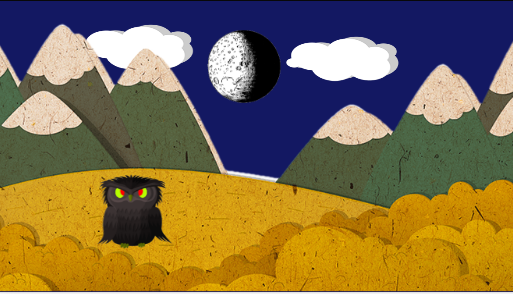
\includegraphics[width=0.8\textwidth]{Figures/ch2/Landscape/final_nigth}
    \caption{Nuestra aplicación nos mostrará un paisaje, en el que podremos cambiar entre noche y día.}
\end{figure}

\subsection{Primeros pasos. El cielo.}


Empezaremos como siempre, creando un nuevo proyecto dentro de nuestro directorio de trabajando utilizando el Ionic CLI. En mi caso, he decidido llamarle Landscape:

\begin{lstlisting}[language=bash]
  # ionic start Landscape blank --v2
\end{lstlisting}

Empezaremos editando los ficheros \emph{home.html} y \emph{home.scss} (podemos renombrar la página con un nombre más descriptivo si queremos, lo cual sería recomendable en caso de tener más páginas, pero en este caso, no será necesario). Eliminaremos todo el contenido de del fichero HTML y añadiremos un \emph{div} que actuara como ``lienzo'' para nuestro paisaje. A este elemento le vamos a asignar las clases \emph{canvas} y \emph{sky}, haciéndolo más reconocible.

\begin{lstlisting}[style=htmlcssjs,frame=tlrb, xleftmargin={0.2cm}]
  <div class="canvas sky" ></div>
\end{lstlisting}

En cuanto al fichero \emph{.scss}, añadiremos los estilos para nuestro nuevo elemento. Estos estilos los anidaremos dentro del elemento \emph{page-home}. El elemento \emph{page-home} es el que representa a nuestro componente (la opción \emph{selector} del metadata de un \emph{@component} es la que indica el nombre de este selector).

\begin{lstlisting}[style=htmlcssjs,frame=tlrb, xleftmargin={0.2cm}]
  page-home {
    .canvas.sky{
      height: 100%;
      width: 100%;
      background-color: #00BFFF;
    }
  }
\end{lstlisting}

Aquí vemos una de las capacidades comentadas de \emph{Sass}. Hemos anidado los estilos que aplican a las clases \emph{.canvas.sky} dentro de \emph{page-home}. Para ver la diferencia con \emph{CSS}, podemos ver el código que esto genera al ser compilado:

\begin{lstlisting}[style=htmlcssjs,frame=tlrb, xleftmargin={0.2cm}]
  page-home .canvas.sky {
    height: 100%;
    width: 100%;
    background-color: #00BFFF;
  }
\end{lstlisting}

Resulta más intuitivo definir los estilos anidando las reglas de igual forma que está definidos los elementos dentro del \gls{DOM} de la página, que la forma que se utiliza en \gls{CSS}, en la que la relación padre e hijos se representa separando los identificadores con un espacio.

Si ejecutamos en estos momentos la aplicación, no veremos más que una pantalla azul, la cual hará la función de cielo en nuestro paisaje. Será sobre este cielo donde iremos añadiendo elementos.

\subsection{Animaciones definidas sobre el componente. El sol y la luna.}


Empezaremos por incluir un sol, y al igual que hicimos con el canvas, este será representado por un componente \gls{HTML} al que le añadiremos como fondo la imagen de un sol. Esta imagen tendremos que ponerla dentro de la carpeta \emph{/src/assets} para que, una vez se genere la aplicación, esta sea incluida. Yo he creado una carpeta intermedia llamada \emph{landscape} para tener las imágenes mas ordenadas. Así pues, añadimos el sol dentro de nuestro ``lienzo'' y lo estilamos dentro de nuestro fichero \emph{scss}:

\noindent
\begin{minipage}[t]{.48\textwidth}
{\begin{lstlisting}[title={home.html}, style=htmlcssjs,frame=tlrb,xleftmargin={0.2cm}]
<div class="canvas sky" >
  <div class="celestial sun" ></div>
</div>
\end{lstlisting}}
\end{minipage}\hfill
\noindent
\begin{minipage}[t]{.48\textwidth}
{\begin{lstlisting}[title={home.scss}, style=htmlcssjs,frame=tlrb,xleftmargin={0.2cm}]
page-home {
 .canvas.sky{ ... }
 .celestial{
     position: fixed;
     height: 100px;
     width: 100px;
     left: 40%;
     top: 10%;
     background-size: contain;
     background-repeat: no-repeat;
     &.sun{
       background-image: url(../assets/landscape/sun.png);
     }
   }
}
\end{lstlisting}}
\end{minipage}

Si nos fijamos, he asignado dos clases al elemento que contendrá mi sol, la clase \emph{celestial} y la clase \emph{sun}. A estas clases las he dado estilo anidando la clase \emph{sun} dentro de la clase \emph{celestial}, pero con un elemento diferente a la de otras anidaciones. En el caso de la clase \emph{sun}, le he antepuesto el carácter \emph{\&}. ¿Y qué significa esto?. A la hora de generar el fichero \emph{CSS}, el compilador sustituirá este carácter por el selector del estilo padre, es decir, por \emph{.celestial}. Para que nos hagamos una mejor idea:

\begin{tikzpicture}[>=stealth, thick]

\node (A) at (-4,0) [draw, process, text width=5cm, minimum height=0.5cm, align=flush center]
{
.celestial \{
  .sun \{ ... \}
\}
};

\node (B) at (4, 0) [draw, process, minimum height=0.5cm, align=flush center]
{
.celestial .sun \{ ... \}
};

\node (C) at (-4, -1) [draw, process, text width=5cm, minimum height=0.5cm, align=flush center]
{
.celestial \{
  \&.sun \{ ... \}
\}
};

\node (D) at (4, -1) [draw, process, minimum height=0.5cm, align=flush center]
{
.celestial.sun \{ ... \}
};

\draw[->] (A) -- node[above]{Compila a} (B);
\draw[->] (C) -- node[above]{Compila a} (D);
\end{tikzpicture}

Con esto conseguimos tener nuestro sol en medio del cielo azul, pero uno de los comportamientos que buscamos es que nuestro paisaje tenga una versión nocturna  además de una diurna. Para hacer esto, vamos a definir un estado dentro de nuestro \emph{@component} que defina si es de día, o de noche, y haremos que este estado cambie al pulsar sobre nuestro sol. Para esto solo será necesario vincular el evento de \emph{click} sobre el sol a una función que haga cambiar la variable de estado de nuestro componente:

\noindent
\begin{minipage}[t]{.48\textwidth}
{\begin{lstlisting}[style=htmlcssjs,frame=tlrb, xleftmargin={0.2cm}]
<div class="canvas sky" >
  <div class="celestial sun" (click)="toogleState()" ></div>
</div>
\end{lstlisting}}
\end{minipage}\hfill
\noindent
\begin{minipage}[t]{.48\textwidth}
{\begin{lstlisting}[style=htmlcssjs,frame=tlrb, xleftmargin={0.2cm}]
export class HomePage {
  state: string = 'day';

  // otras funciones

  toogleState() {
    this.state = 'day' == this.state ? 'night' : 'day';
  }
}
\end{lstlisting}}
\end{minipage}

Ya tenemos una variable que almacena el estado y que podemos cambiar pulsando nuestro sol, pero no vemos como esto se refleja en nuestro paisaje (a no ser que depuremos la aplicación o hagamos que imprima el valor por consola). Vamos por fín a hacer uso de las animaciones. La primera va a ser muy sencillita, cambiar el color del cielo a uno mas nocturno. En primer lugar vamos a crear una animación de Angular que haga esto y la añadiremos a nuestro componente. Para hacer esto modificamos el metadata de nuestro componente de la siguiente manera:

{\begin{lstlisting}[style=htmlcssjs,frame=tlrb, xleftmargin={0.2cm}]
@Component({
  selector: 'page-home',
  templateUrl: 'home.html',
  animations: [
    trigger('skyState', [
      state('day', style({
        backgroundColor: '#00BFFF'
      })),
      state('night',   style({
        backgroundColor: '#131862'
      })),
      transition('day <=> night', animate('1s')),
    ]),
  ]
})
\end{lstlisting}}

No nos olvidemos de importar las nuevas clases que vamos a utilizar: https://angular.io/docs/ts/latest/api/core/index/trigger-function.html

{\begin{lstlisting}[style=htmlcssjs,frame=tlrb, xleftmargin={0.2cm}]
import { Component, ElementRef, ViewChild, AfterViewInit, trigger, state, style, transition, animate} from '@angular/core';
\end{lstlisting}}

Veamos que es lo hemos definido:

\begin{enumerate}
  \item Hemos definido el metadato \emph{animations} de nuestro componente como una lista en la que de momento solo definiremos un \emph{trigger}\footnote{\url{https://angular.io/docs/ts/latest/api/core/index/trigger-function.html}}.
  \item Este \emph{trigger}, que es una llamada al constructor de la clase \emph{trigger}, lo hemos nombrado \emph{skyState} (primer parámetro que acepta el constructor).
  \item Como segundo parámetro le pasamos una lista de estados y transiciones que definen las animaciones.
  \item Hemos definido dos estados mediante la clase \emph{state}\footnote{\url{https://angular.io/docs/ts/latest/api/core/index/state-function.html}}:
  \begin{enumerate}
    \item Un estado llamado \emph{day}, con un estilo que define el color de fondo de la misma manera que se definen las reglas en \gls{CSS}.
    \item Un estado llamado \emph{night}, que también define también el color de fondo, pero cambiando el valor de este.
  \end{enumerate}
  \item Junto a los estados hemos definido una transición. Como primer parámetro, le pasamos el nombre de los estados definidos previamente entre los que se hace el cambio, y la dirección entre ellos en las que se da (la flecha <=> indica bidireccionalidad, mientras que una flecha tipo =>, indicaría solo un sentido). Como segundo parámetro, seleccionamos el tipo de animación que queremos mediante una clase \emph{animate}\footnote{\url{https://angular.io/docs/ts/latest/api/core/index/animate-function.html}}, en este caso, queremos que la animación dure un segundo en completarse ('1s').
\end{enumerate}

Por último nos quedaría vincular nuestro \emph{trigger} a nuestro cielo y al estado definido dentro del componente. Esto se hace directamente editando el elemento \gls{HTML}.

{\begin{lstlisting}[style=htmlcssjs,frame=tlrb, xleftmargin={0.2cm}]
<div class="canvas sky" [@skyState]="state" >
\end{lstlisting}}

Que el sol aparezca en medio de un cielo nocturno no es muy común, necesitaremos hacer uso de otra animación para solucionar esto. En esta ocasion en vez de contar con un único elemento al que le cambiamos el estilo, añadiremos uno nuevo que representará la luna. Este elemento tendrá varios estilos en común con el sol definido anteriormente, por lo que compartirán clase \emph{celestial} (ahora le vemos el sentido a la separación de estilos que hicimos anteriormente entre \emph{celestial} y \emph{sun}). El ver aparecer o desaparecer estos cuerpos celestiales en centro de la pantalla no es lo más bonito, así que para esta animación haremos que el cuerpo celeste aparezca por el borde superior, y desaparezca por el borde inferior según le toque. Nos vamos a ayudar de la regla \emph{top} que define \gls{CSS}, con la cuál podemos definir a que distancia respecto al borde superior se posiciona el elemento en cuestión (de igual manera, la regla \emph{left} define la distancia respecto al borde izquierdo). Entre los valores que acepta, se puede indicar un tanto por ciento respecto a la altura del elemento padre y así, jugando con este valor, podremos crear la animación que queremos. Empezamos definiendo nuestro nuevo elemento y las posiciones de origen.

\noindent
\begin{minipage}[t]{.48\textwidth}
{\begin{lstlisting}[style=htmlcssjs,frame=tlrb, xleftmargin={0.2cm}]
<div class="canvas sky" [@skyState]="state" >
  <div #sun class="celestial sun" (click)="toogleState()" ></div>
  <div #moon class="celestial moon" (click)="toogleState()" ></div>
</div>
\end{lstlisting}}
\end{minipage}\hfill
\noindent
\begin{minipage}[t]{.48\textwidth}
{\begin{lstlisting}[style=htmlcssjs,frame=tlrb, xleftmargin={0.2cm}]
.celestial{
  position: fixed;
  height: 100px;
  width: 100px;
  left: 40%;
  top: 10%;
  background-size: contain;
  background-repeat: no-repeat;
  &.sun{
    background-image: url(../assets/landscape/sun.png);
  }
  &.moon{
    background-image: url(../assets/landscape/moon.png);
  }
}
\end{lstlisting}}
\end{minipage}

Crearemos una animación que será la que usen ambos elementos, ambos cuerpos celestiales. En esta animación usaremos dos estados, pero no definiremos ninguno ¿Cómo es esto posible?. Angular ya define dos estados especiales, a saber:

\begin{enumerate}
  \item El estado \emph{void}, que se define un el estado de los elementos que desaparecen.
  \item El estado \emph{*}, es un estado comodín para cuando no existe estado definido.
\end{enumerate}

Con esto presente, crearemos una animación para los siguientes cambios de estado:

\begin{enumerate}
  \item void => *: Esta transición definirá la entrada.
  \item * => *: Por el contrario, esta definirá la salida.
\end{enumerate}

{\begin{lstlisting}[style=htmlcssjs,frame=tlrb, xleftmargin={0.2cm}]
animations: [
  trigger('skyState', [ ... ]),
  trigger('flyInOut', [
    transition('void => *', [
      style({top: '-100%'}),
      animate('1s')
    ]),
    transition('* => void', [
      animate('1s', style({top: '100%'}))
    ])
  ]),
]
\end{lstlisting}}

\notebox{El uso de animaciones de entrada y salida es frecuente, por ello en Angular se han asignado alias especiales a estos cambios de estado. En las transiciones, podemos cambiar la definición de cambio de estado \textbf{'void => *'} por \textbf{':enter'} y \textbf{'* => void'} por \textbf{':leave'}.}

En la transición de entrada, al definir un estilo dentro de la transición, hacemos que antes de que se inicie esta, se le aplique el estilo definido. Así conseguimos que nuestro elemento se coloque por encima de la pantalla. Por el contrario, en la transición de salida, el estilo está definido dentro de la animación. Indicamos así el estilo al finalizar la animación. Este estilo no se guarda, si no que al terminar la animación, el estilo es borrado del elemento.

Solo nos queda asignar la animación a nuestros elementos, pero en esta ocasión no hay estados propiamente dichos, si no que hay que hacer que el elemento aparezca y desaparezca, ¿Cómo hacemos esto?. Usaremos la directriz de Angular \textbf{ngIf}. Esta directriz hace que aparezca o no el elemento asignado en escena según si el valor asignado es \emph{true} o \emph{false}. Usando esta directriz, y la propiedad \emph{state} definida en el componente, nos será fácil conseguir nuestro objetivo:

{\begin{lstlisting}[style=htmlcssjs,frame=tlrb, xleftmargin={0.2cm}]
<div class="canvas sky" [@skyState]="state" >
  <div class="celestial sun" [@flyInOut] *ngIf="state === 'day'" (click)="toogleState()" ></div>
  <div class="celestial moon" [@flyInOut] *ngIf="state === 'night'" (click)="toogleState()" ></div>
</div>
\end{lstlisting}}

\subsection{Animación mediante código JavaScript/TypeScript. El terreno.}


Ya va cogiendo forma nuestro paisaje. Lo siguiente que vamos a añadir va a ser el terreno. Para que nuestro terreno sea un poco más interactivo, vamos a hacer que podamos moverlo con el dedo tanto a la izquierda, como a la derecha. Esto no podemos hacerlo usando las animaciones, ya que el desplazamiento del dedo no es siempre el mismo y las animaciones necesitan tener definido un inicio y un fin. Por tanto, debemos de tratar este movimiento desde el código JavaScript (o TypeScript como en nuestro caso). El gesto de mover un dedo sobre un elemento de nuestra página provoca que se genere un evento JavaScript, que como otro cualquiera, podemos capturar en nuestro código. Este evento nos da información sobre el recorrido que ha hecho nuestro dedo sobre la pantalla, y usando esta información, podremos variar en consecuencia la posición del elemento que representa el terreno.

Vamos a empezar como es normal añadiendo el elemento a nuestro código \gls{HTML} y dándole el estilo deseado.

\noindent
\begin{minipage}[t]{.48\textwidth}
{\begin{lstlisting}[style=htmlcssjs,frame=tlrb, xleftmargin={0.2cm}]
<div class="canvas sky" [@skyState]="state" >
  <div class="celestial sun" [@flyInOut] *ngIf="state === 'day'" (click)="toogleState()" ></div>
  <div class="celestial moon" [@flyInOut] *ngIf="state === 'night'" (click)="toogleState()" ></div>
  <div #landscape class="landscape" ></div>
</div>
\end{lstlisting}}
\end{minipage}\hfill
\noindent
\begin{minipage}[t]{.48\textwidth}
{\begin{lstlisting}[style=htmlcssjs,frame=tlrb, xleftmargin={0.2cm}]
page-home { ... }
  .celestial{ ... }
  .landscape {
    position: fixed;
    height: 100vh;
    width: calc(100vh*1024/373); // El tamano de la imagen es 1024*373, asi que calculamos la relacion alto entre ancho
    background-image: url(../assets/landscape/landscape.png);
    background-size: auto 100%;
    background-repeat: no-repeat;
    pointer-events: none;
  }
}
\end{lstlisting}}
\end{minipage}

Ya que el \emph{div} que contiene la imagen cubre nuestro \emph{sol/luna}, aunque sea con zona transparente, interfiere en el evento del click, evitando que llegue a nuestro cuerpo celeste. Para solucionarlo, añadimos la regla \emph{pointer-events: none;} y controlaremos el evento de pulsación con el dedo desde el  \emph{div} del elemento \emph{canvas}.

Si nos fijamos, en nuestro nuevo \emph{div} aparece un atributo que no habíamos usado anteriormente, \emph{\#landscape}. Al añadir un atributo prefijadocon el caracter almohadilla (\#), le estamos asignando un identificador gracias al cual podremos hacer uso de este elemento desde dentro del \emph{component} y poder ``jugar'' con él. Ya que el tamaño de nuestro terreno se ajusta según la altura de la pantalla, necesitaremos calcular de manera programática el máximo desplazamiento horizontal para evitar que el terreno desaparezca por uno de los bordes laterales. Para hacer esto, es necesario que la vista este renderizada (y por tanto los tamaños ajustados en el momento de realizar los cálculos que veremos a continuación). Para esta tarea, Angular cuenta con un componente \emph{AfterViewInit} el cual debemos implementar en nuestro componente, junto con el método \emph{ngAfterViewInit} que se ejecuta al finalizar el renderizado de la pagina.

\notebox{Angular controla un ciclo de vida para cada uno de los componentes que definimos, y nos provee a los desarrolladores de los mecanismos necesarios para poder realizar acciones en los diferentes momentos de este ciclo. En el caso que nos ocupa, nos interesa el momento una vez que la página ha sido dibujada, pero existen más. Para mas información sobre este ciblo, consultar la \gls{API}\footnote{\url{https://angular.io/docs/ts/latest/guide/lifecycle-hooks.html}} de Angular referente a ello. }

El siguiente dibujo muestra nuestro terreno a modo de croquis donde podemos ver los parámetros que vamos a necesitar calcular para poder implementar el movimiento:

\begin{tikzpicture}
  \draw [<->] (0,7) -- node[above] {Ancho total del terreno} ++(12,0);
  \draw [<->] (0,6.5) -- node[above] {Recorrido máximo} ++(4,0) ;
  \draw [<->] (4,6.5) -- node[above] {Ancho total de la pantalla} ++(8,0);
  \draw (0,0) rectangle (12,6);
  \filldraw[fill=cyan, draw=black]  (4,0) rectangle (12,6);
  \fill[fill=green, draw=black] plot [smooth] coordinates {(0,0) (3,4) (6,1) (9,4) (12,0)};
  \draw [line width=1mm, red ] (4,0) rectangle (12,6);
  \draw [<->] (0,-0.5) -- node[below] {maxDeltaX} ++(4,0) ;
  \draw [<->] (4,-0.5) -- node[below] {screenWidth} ++(8,0);
  \draw [<->] (0,-1) -- node[below] {landWidth} ++(12,0);
\end{tikzpicture}

Estos valores pueden ser calculados y almacenados como propiedades del componente de la siguiente manera:

{\begin{lstlisting}[style=htmlcssjs,frame=tlrb, xleftmargin={0.2cm}]
export class HomePage implements AfterViewInit {
  /* Resto de variables */
  @ViewChild('landscape') landscapeElement:ElementRef; //nuestro div al que identificamos con el atributo #landscape
  maxDeltaX:number;
  currentDeltaX: number;
  lastPanDeltaX: number = 0;

  ngAfterViewInit() {
    var landWidth = this.landscapeElement.nativeElement.clientWidth;
    var screenWidth = this.landscapeElement.nativeElement.parentElement.clientWidth;
    this.maxDeltaX = (landWidth - screenWidth) * -1;
    this.currentDeltaX = this.maxDeltaX / 2; // Aprovechamos para centrar el terreno al iniciar.
  }
  /* Resto de funciones */
}
\end{lstlisting}}

\warningbox{Hay que tener en cuenta que el máximo desplazamiento se dará hacia la izquierda, por eso se trata de un número negativo. }

Con las medidas ya calculadas, vamos a tratar el gesto de desplazar el dedo sobre la pantalla. Ionic2 permite vincular los siguientes gestos desde el \emph{HTML}: \textbf{tap, press, pan, swipe, rotate y pinch}. Para nuestro propósito, el evento que necesitamos capturar es el de \textbf{pan} y lo haremos del mismo modo que capturamos el evento de click.

{\begin{lstlisting}[style=htmlcssjs,frame=tlrb, xleftmargin={0.2cm}]
<div class="canvas sky" [@skyState]="state" (pan)="panEvent(\$event)" >
  <div class="celestial sun" [@flyInOut] *ngIf="state === 'day'" (click)="toogleState()" ></div>
  <div class="celestial moon" [@flyInOut] *ngIf="state === 'night'" (click)="toogleState()" ></div>
  <div #landscape class="landscape" ></div>
</div>
\end{lstlisting}}

Veamos primero el código del método \emph{panEvent}, que es la que recoge y trata el gesto, y a continuación explicaré su funcionamiento.

{\begin{lstlisting}[style=htmlcssjs,frame=tlrb, xleftmargin={0.2cm}]
panEvent(e) {
  if (e.eventType == 4) {
    this.lastPanDeltaX = 0;
    return true;
  };
  var dx = e.deltaX - this.lastPanDeltaX;
  this.lastPanDeltaX = e.deltaX;

  if ((this.currentDeltaX + dx) < this.maxDeltaX || (this.currentDeltaX + dx) > 0) {
    return true;
  }
  this.currentDeltaX += dx;

  return true;
}
\end{lstlisting}}

Para entender este código hay que saber como funciona el evento que estamos capturando. Cada vez que se desplaza el dedo sobre la pantalla, por pocos píxeles que sean, se genera un evento que podemos capturar. Esto quiere decir que en caso de mover el dedo sin parar, el evento saltara cada pocos milisegundos. ¿Y que información nos proporciona?. Entre los múltiples parámetros\footnote{\url{https://hammerjs.github.io/api/\#event-object}} que tiene asociado el evento, el que nos indica el desplazamiento es \emph{deltaX} (también nos encontramos con los parámetros \emph{deltaY} y con \emph{distance}, pero en nuestro caso, solo nos interesa el movimiento horizontal). Este parámetro se mide en píxeles y representa la distancia recorrida horizontalmente desde el inicio del gesto. Como nos interesa actualizar la posición del terreno cada vez que se genera el evento para así conseguir que el dibujo se mueva al mismo tiempo que el dedo, necesitamos saber la distancia recorrida no al punto de inicio del gesto, si no al punto en el que se produjo el evento anterior. Para eso calculamos la diferencia entre la \emph{deltaX} del evento anterior, que guardamos en la variable \emph{lastPanDeltaX}, y la \emph{deltaX} del evento actual. Esta diferencia es la que se aplica al desplazamiento actual del terreno (\emph{currentDeltaX}) siempre y cuando entre dentro del desplazamiento permitido (de \emph{mapxDeltaX} a 0). ¿Y cuándo termina el gesto?. Cuando el usuario levanta el dedo, se lanza un último evento en el que el parámetro \emph{eventType}\footnote{\url{https://hammerjs.github.io/api/\#input-events}} toma el valor 4. En este momento, reseteamos \emph{lastPanDeltaX}.

Ahora que tenemos el desplazamiento que tenemos que aplicar a nuestro terreno, nos falta justamente eso, aplicárselo. Angular nos permite modificar el estilo de un elemento según una variable desde el HTML. Para realizar un desplazamiento lateral vamos a aplicar una transformación\footnote{\url{https://www.w3schools.com/cssref/css3_pr_transform.asp}} a nuestro elemento, mas concretamente, \emph{translateX()}, al cual se le pasa el desplazamiento medido en píxeles.

Normalmente para cambiar un estilo según el valor de una variable con Angular se haría lo siguiente:

{\begin{lstlisting}[style=htmlcssjs,frame=tlrb, xleftmargin={0.2cm}]
  <div [style.CSS_PROPERTY_NAME]=" VARIABLE " ></div>
\end{lstlisting}}

Pero en el caso del \emph{tranform}, esto viola algunas directivas de seguridad que aplica Angular, y es que sí, una de las cosas que Angular nos proporciona es protección contra las vulnerabilidades comunes que suelen tener las aplicaciones web \ldots aunque en esta ocasión interfiera con nuestros planes. Por suerte, existen mecanismos para saltarnos estas medidas de seguridad (bajo nuestra responsabilidad) para casos como el que nos ocupa. Estos mecanismos son conocidos como \emph{bypass}\footnote{\url{https://angular.io/docs/ts/latest/api/platform-browser/index/DomSanitizer-class.html}} y previenen de que el valor que les pasemos sea comprobado por los mecanismos de seguridad de Angular.

Para intentar dejar nuestro código lo más limpio posible, crearemos una tubería (ya vimos que son en la práctica del \nameref{sec:crono}) que al pasarle el valor numérico, nos genere el valor a asignar a la propiedad \emph{transform}.

{\begin{lstlisting}[style=htmlcssjs,frame=tlrb, xleftmargin={0.2cm}]
import { Pipe, PipeTransform } from '@angular/core';
import { DomSanitizer } from '@angular/platform-browser';

@Pipe({name: 'transform_sanitizer'})
export class TransformSanitizer implements PipeTransform {

  constructor(private sanitizer:DomSanitizer){}

  transform(deltaX) {
    return this.sanitizer.bypassSecurityTrustStyle("translateX(" + deltaX + "px)");
  }
}
\end{lstlisting}}

Ya solo nos quedaría añadirlo a nuestro \emph{HTML}:

{\begin{lstlisting}[style=htmlcssjs,frame=tlrb, xleftmargin={0.2cm}]
<div class="canvas sky" [@skyState]="state" (pan)="panEvent(\$event)" >
  <div class="celestial sun" [@flyInOut] *ngIf="state === 'day'" (click)="toogleState()" ></div>
  <div class="celestial moon" [@flyInOut] *ngIf="state === 'night'" (click)="toogleState()" ></div>
  <div #landscape [style.transform]="currentDeltaX | transform_sanitizer" class="landscape" ></div>
</div>
\end{lstlisting}}

\subsection{Animación CSS. El ave.}

Nuestro siguiente paso será incluir un habitante en nuestro paisaje, yo me he decantado por un pájaro. Nuestro nuevo amigo estará de pie sobre el terreno, por ello, es necesario que se mueva cuando desplacemos todo el terreno. Para conseguirlo, el elemento que representa a este pájaro dentro del \emph{div} del terreno. Veamos el código:

\noindent
\begin{minipage}[t]{.48\textwidth}
{\begin{lstlisting}[style=htmlcssjs,frame=tlrb, xleftmargin={0.2cm}]
<div class="canvas sky" [@skyState]="state" (pan)="panEvent(\$event)" >
  <div class="celestial sun" [@flyInOut] *ngIf="state === 'day'" (click)="toogleState()" ></div>
  <div class="celestial moon" [@flyInOut] *ngIf="state === 'night'" (click)="toogleState()" ></div>
  <div #landscape [style.transform]="currentDeltaX | transform_sanitizer" class="landscape" >
    <div class="bird" [@birdState]="state" ></div>
  </div>
</div>
\end{lstlisting}}
\end{minipage}\hfill
\noindent
\begin{minipage}[t]{.48\textwidth}
{\begin{lstlisting}[style=htmlcssjs,frame=tlrb, xleftmargin={0.2cm}]
page-home {
  .canvas.sky{ ... }
  .celestial{ ... }
  .landscape {
    // Resto de propiedades.
    .bird {
      position: fixed;
      height: 100px;
      width: 100px;
      left: 30%;
      top: 60%;
      background-size: 100% 100%;
      background-repeat: no-repeat;
      pointer-events: none;
    }
  }
}
\end{lstlisting}}
\end{minipage}

Ya que la fauna diurna no es la misma que la que nos encontramos en la noche, vamos a cambiar la especie de nuestro habitante utilizando una animación que modifique la imagen que se utiliza:

{\begin{lstlisting}[style=htmlcssjs,frame=tlrb, xleftmargin={0.2cm}]
trigger('birdState', [
  state('day', style({
    'background-image': 'url(../assets/landscape/bird.png)'
  })),
  state('night',   style({
    'background-image': 'url(../assets/landscape/owl.png)'
  })),
  transition('day <=> night', animate('0.5s 0.5s')), // La animación dura 0.5 segundos y empiza 0.5 segundos retrasada
]),
\end{lstlisting}}

Para animar un poco a nuestro pájaro, y no parezca que se trata de una objeto sin vida, vamos a añadirle un poco de movimiento, y como no, vamos a usar una animación para esto. En este caso, al tratarse de una animación que se repite en el tiempo y de la que conocemos tanto su estado inicial como final e intermedios, definiremos la animación directamente en el \gls{CSS}. Vamos a definir dos animaciones diferentes, durante el día, nuestro pájaro pivoteará de un lado a otro, y durante la noche, pegará saltos. \gls{CSS} nos permite definir \emph{keyframes}, en los que indicar el estilo según el porcentaje de animación que se haya completado.

{\begin{lstlisting}[style=htmlcssjs,frame=tlrb, xleftmargin={0.2cm}]
@keyframes spin {
    0%, 45%   {transform: rotateY(0deg);} // En el 45% empezará a cambiar
    50%, 95%  {transform: rotateY(180deg);} // En el 50% ya se habrá realizado el cambio
}

@keyframes jump {
    0%, 45%, 55%   {top: 60%}
    50%  {top: 50%} // Al punto más alto se llega a mitad de la animación
}
\end{lstlisting}}

Completamos el estilo de nuestro elemento para añadir la animación. En este caso le pondremos por defecto la animación \emph{spin} (y así ver en conjunto todas las opciones de la animación), aunque como veremos a continuación, esta animación cambiará junto al estado.

{\begin{lstlisting}[style=htmlcssjs,frame=tlrb, xleftmargin={0.2cm}]
.bird {
  position: fixed;
  height: 100px;
  width: 100px;
  left: 30%;
  top: 60%;
  background-size: 100% 100%;
  background-repeat: no-repeat;
  pointer-events: none;
  animation-name: spin;
  animation-duration: 6s;
  animation-iteration-count: infinite;
  animation-timing-function: easeInQuint // https://www.w3schools.com/cssref/css3_pr_animation-timing-function.asp;
}
\end{lstlisting}}

En nuestro componente cambiamos la definición del trigger \emph{birdState}:

{\begin{lstlisting}[style=htmlcssjs,frame=tlrb, xleftmargin={0.2cm}]
trigger('birdState', [
  state('day', style({
    'background-image': 'url(../assets/landscape/bird.png)',
    'animation-name': 'spin',
    'animation-duration': '6s'
  })),
  state('night',   style({
    'background-image': 'url(../assets/landscape/owl.png)',
    'animation-name': 'jump',
    'animation-duration': '3s'
  })),
  transition('day <=> night', animate('0.5s 0.5s')),
])
\end{lstlisting}}

Veamos como funciona la animación de giro con la configuración especificada. En primer lugar, la animación durará 6s. Esto, junto con la definición del \emph{keyframe} tenemos que:

\begin{enumerate}
  \item El elemento empieza rotado 0 grados.
  \item En el segundo 6*0.45 = 2.7, empieza la animación de giro.
  \item En el segundo 6*0.5 = 3, el elemento está rotado 180 grados.
  \item En el segundo 6*0.95 = 5.7, el elemento empieza a rotar hacia la posición original.
  \item En el segundo 6*1 = 6, el elemento está en la posición original.
  \item Vuelta a empezar.
\end{enumerate}

El funcionamento es análoco en la definición del salto.

\subsection{Elementos extras. Sonidos y nubes.}


Como broche final a nuestro paisaje, vamos a hacer que se reproduzca un sonido, en nuestro caso el canto del pájaro, cuando se realiza el cambio de estado. Las animaciones de Angular permiten asignar desde el \emph{HTML} una acción tanto al comienzo de la animación, como al finalizarla.

{\begin{lstlisting}[style=htmlcssjs,frame=tlrb, xleftmargin={0.2cm}]
<div #landscape [style.transform]="currentDeltaX | transform_sanitizer" class="landscape" >
  <div #bird class="bird" (@birdState.start)="playAudio() " [@birdState]="state" ></div>
</div>
\end{lstlisting}}

{\begin{lstlisting}[style=htmlcssjs,frame=tlrb, xleftmargin={0.2cm}]
export class HomePage implements AfterViewInit {
  //Resto de variables
  audio: any;

  //Resto de funciones
  playAudio() {
    if (this.audio) { //Nos aseguramos de que si existe algún sonido reproduciéndose, lo detenemos
      this.audio.pause();
    }
    this.audio = 'day' == this.state ? new Audio('../assets/sounds/bird.mp3') : new Audio('../assets/sounds/owl.mp3');
    this.audio.play();
  }
}
\end{lstlisting}}

Con esto ya tendríamos completo nuestro paisaje. Podemos añadir más elementos si queremos poner en práctica lo aprendido o probar cosas nuevas, por ejemplo, yo he añadido unas nubes que también se mueven junto con el terreno, pero a una velocidad menor.

\noindent
\begin{minipage}[t]{.48\textwidth}
{\begin{lstlisting}[style=htmlcssjs,frame=tlrb, xleftmargin={0.2cm}]
<div class="canvas sky" [@skyState]="state" (pan)="panEvent(\$event)" >
  <div class="celestial sun" [@flyInOut] *ngIf="state === 'day'" (click)="toogleState()" ></div>
  <div class="celestial moon" [@flyInOut] *ngIf="state === 'night'" (click)="toogleState()" ></div>
  <div [style.transform]="currentDeltaX / 3 | transform_sanitizer" class="cloud left" ></div>
  <div [style.transform]="currentDeltaX / 3 | transform_sanitizer" class="cloud rigth" ></div>
  <div #landscape [style.transform]="currentDeltaX | transform_sanitizer" class="landscape" >
    <div class="bird" (@birdState.start)="playAudio()" [@birdState]="state" ></div>
  </div>
</div>

\end{lstlisting}}
\end{minipage}\hfill
\noindent
\begin{minipage}[t]{.48\textwidth}
{\begin{lstlisting}[style=htmlcssjs,frame=tlrb, xleftmargin={0.2cm}]
page-home {
  .canvas.sky{ ...
    .celestial{ ... }
    .cloud {
      position: fixed;
      height: 60px;
      width: 150px;
      background-image: url(../assets/landscape/cloud.png);
      background-size: 100% 100%;
      background-repeat: no-repeat;
      pointer-events: none;
      &.left {
        top: 8%;
        left: 25%;
      }
      &.rigth {
        top: 12%;
        left: 65%;
      }
    }
    .landscape { ... }
  }
}
\end{lstlisting}}
\end{minipage}

\subsection{Apunte final y uso de animaciones en otros escenarios.}

Con esta práctica he querido abarcar diferentes formas de crear animaciones cuando se trata de una aplicación hecha con Ionic2. Se puede conseguir el mismo resultado aplicando métodos distintos. Por ejemplo, haciendo las animaciones solo con JS, utilizar jQuery u alguna otra librería externa, \ldots.

Como último apunte, indicar que aunque en este caso hemos estado animando elementos que representaban imágenes para intentar hacer la explicación más visual y llamativa, no debemos pensar que las animaciones solo se utilizan para hacer "dibujitos". Las animaciones se pueden aplicar a cualquier elemento del árbol \gls{DOM} y a cualquier regla que se pueda definir en \gls{CSS}. Un ejemplo muy utilizado sería cambiar el tamaño de fuente en un texto cuándo nos posicionamos sobre él:

{\begin{lstlisting}[style=htmlcssjs,frame=tlrb, xleftmargin={0.2cm}]
<head>
  <style media="screen" >
    .text {
      font-size: 14px;
      transition: font-size 1s ease-in; \\ Manera abreviada de definir una transición
    }
    .text:hover {
      font-size: 40px;
    }
  </style>
</head>
<body>
  <div class="text" >
    Pasa sobre mí el ratón.
  </div>
</body>
\end{lstlisting}}

O desplegar un menú lateral:

{\begin{lstlisting}[style=htmlcssjs,frame=tlrb, xleftmargin={0.2cm}]
<head>
  <style media="screen" >
    body {
      display: flex;
      height: 100%;
    }
    div {
      height: 100%;
    }
    div.menu {
      background-color: green;
      width: 20px;
      transition: width 1s, background-color 1s;
    }
    div.menu:hover {
      background-color: yellow;
      width: 200px;
    }
    div.main {
      background-color: cyan;
      flex-grow: 1;
    }
    button {
      min-width: 200px
    }
  </style>
</head>
<body>
  <div class="menu" >
    <button>OPTION 1</button>
    <button>OPTION 2</button>
    <button>OPTION 3</button>
  </div>
  <div class="main" ></div>
</body>
\end{lstlisting}}

\clearpage
\section{Recordatorios asociados a localizaciones} \label{sec:recordatorios}

En esta última práctica se propone crear una aplicación que permita al usuario gestionar una serie de recordatorios, pero en vez de estar asociados estos recordatorios a un instante de tiempo en concreto, se asocien a un área geográfica concreta. Vamos a definir esta área como una circunferencia de 100 metros de radio alrededor de un punto geográfico que será definido por el usuario cuando cree el recordatorio. A esta circunferencia la llamaremos ``área de influencia''. Para ello, el usuario seleccionara un punto sobre el mapa y asignará un nombre y una descripción para este recordatorio.

\begin{figure}[H]
\centering
    \centering
        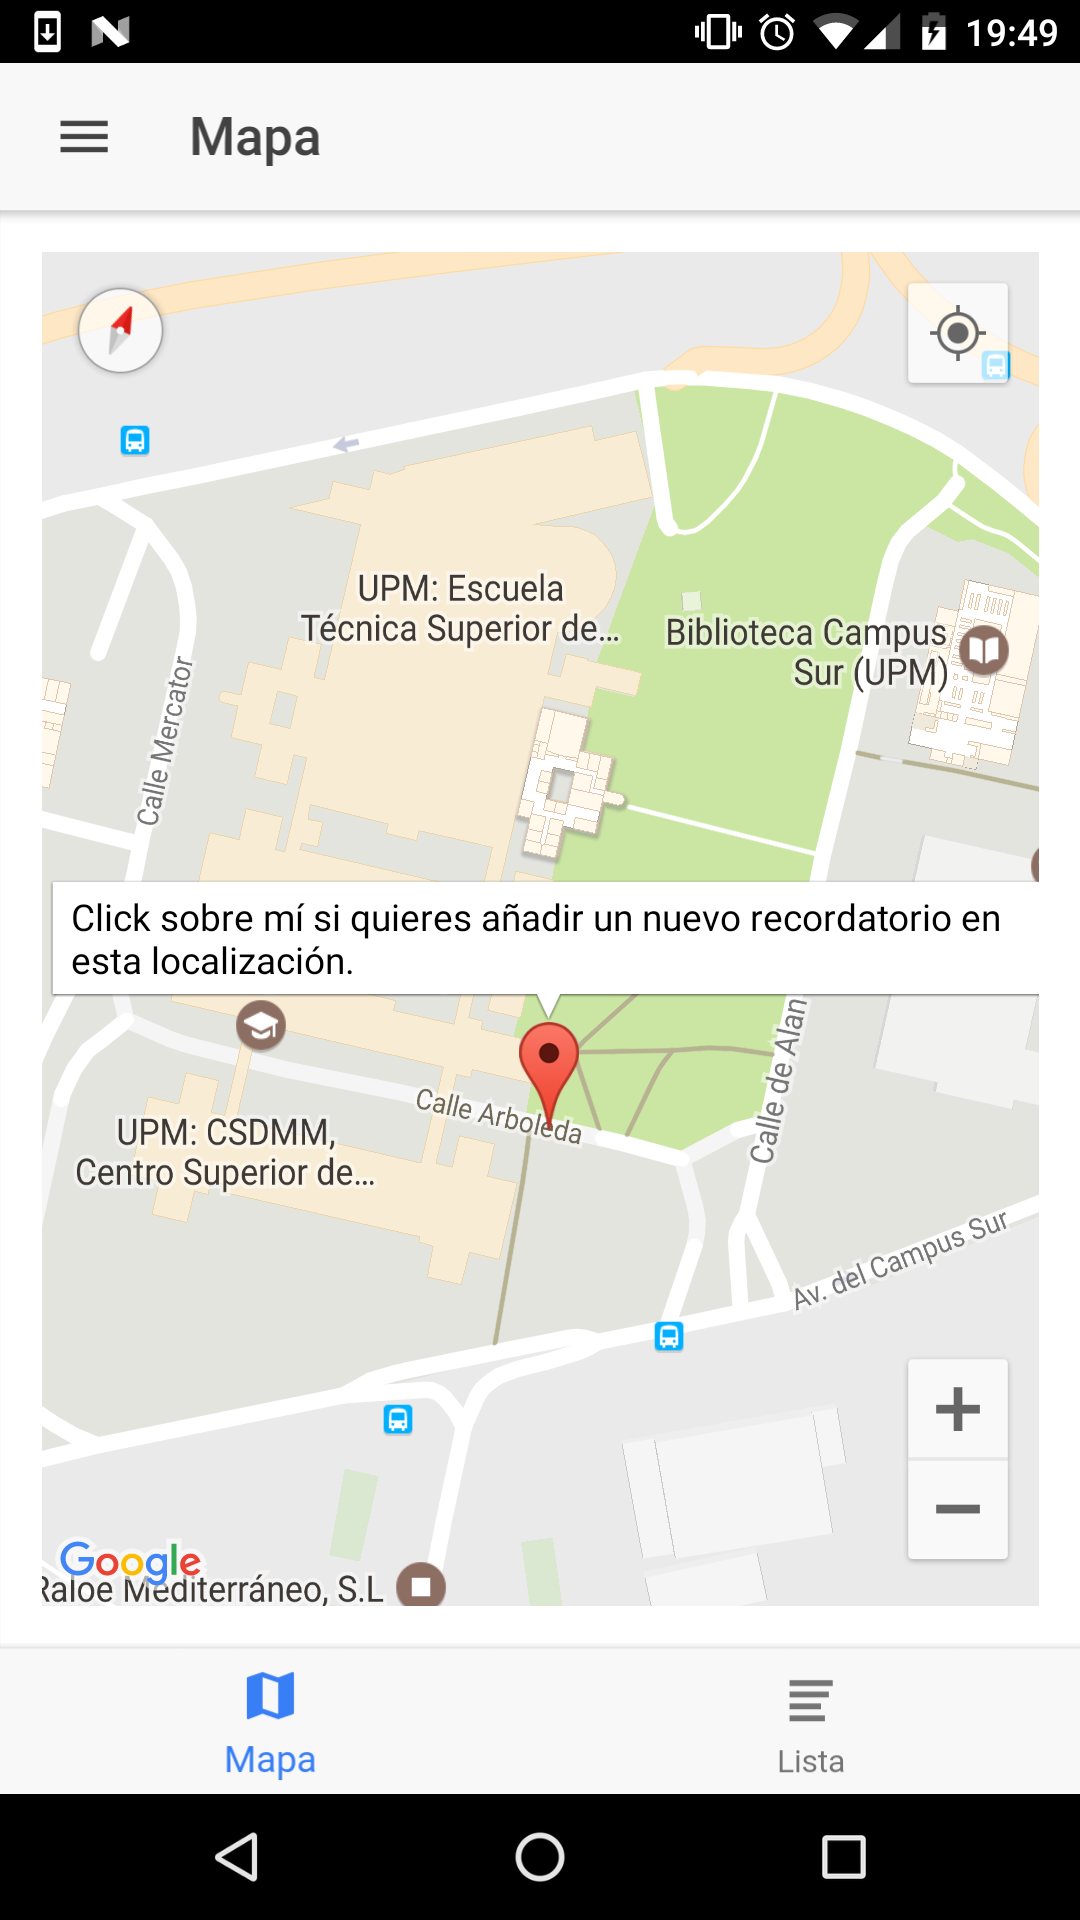
\includegraphics[width=0.4\textwidth]{Figures/ch2/ReminderMap/preview_map_1}
        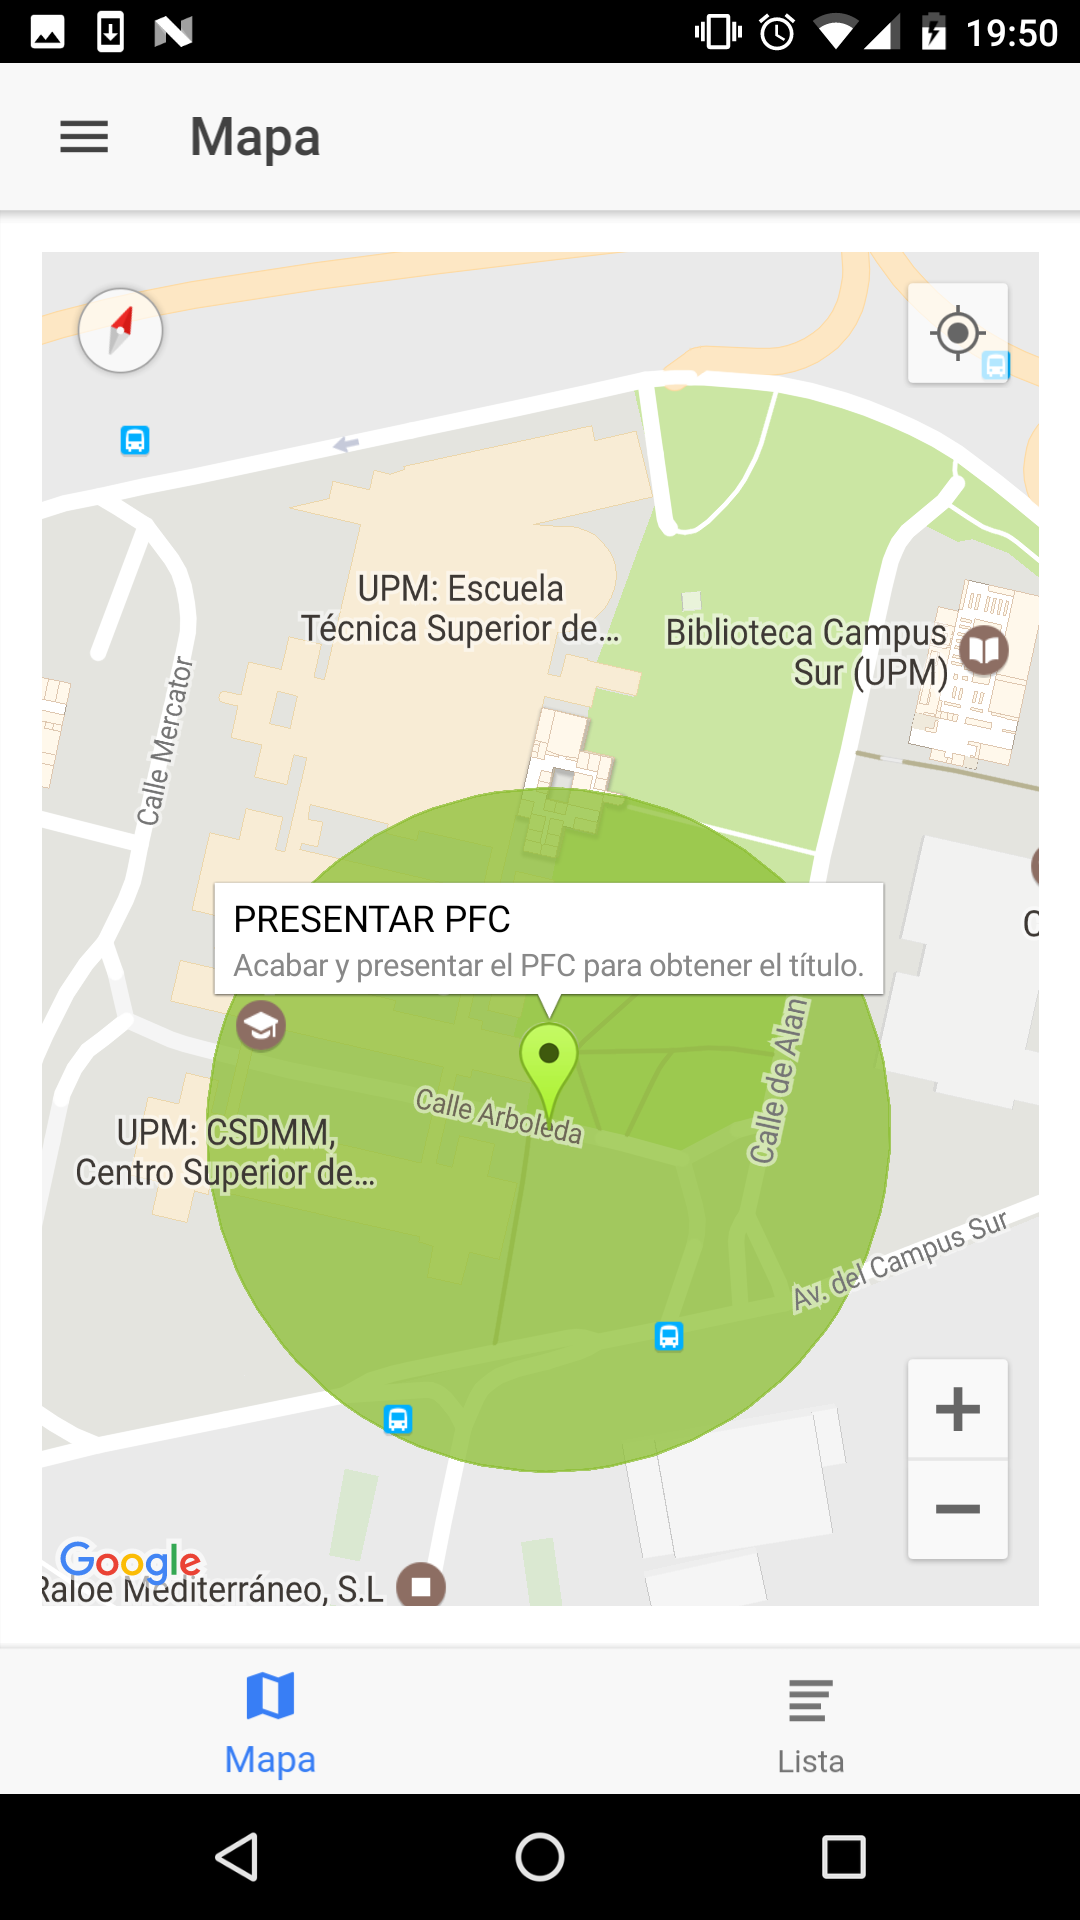
\includegraphics[width=0.4\textwidth]{Figures/ch2/ReminderMap/preview_map_2}
    \caption{Así se vería el mapa, con los recordatorios marcados.}
\end{figure}

También podremos ver estos recordatorios listados, pudiendo interactuar con ellos:

\begin{figure}[H]
\centering
    \centering
        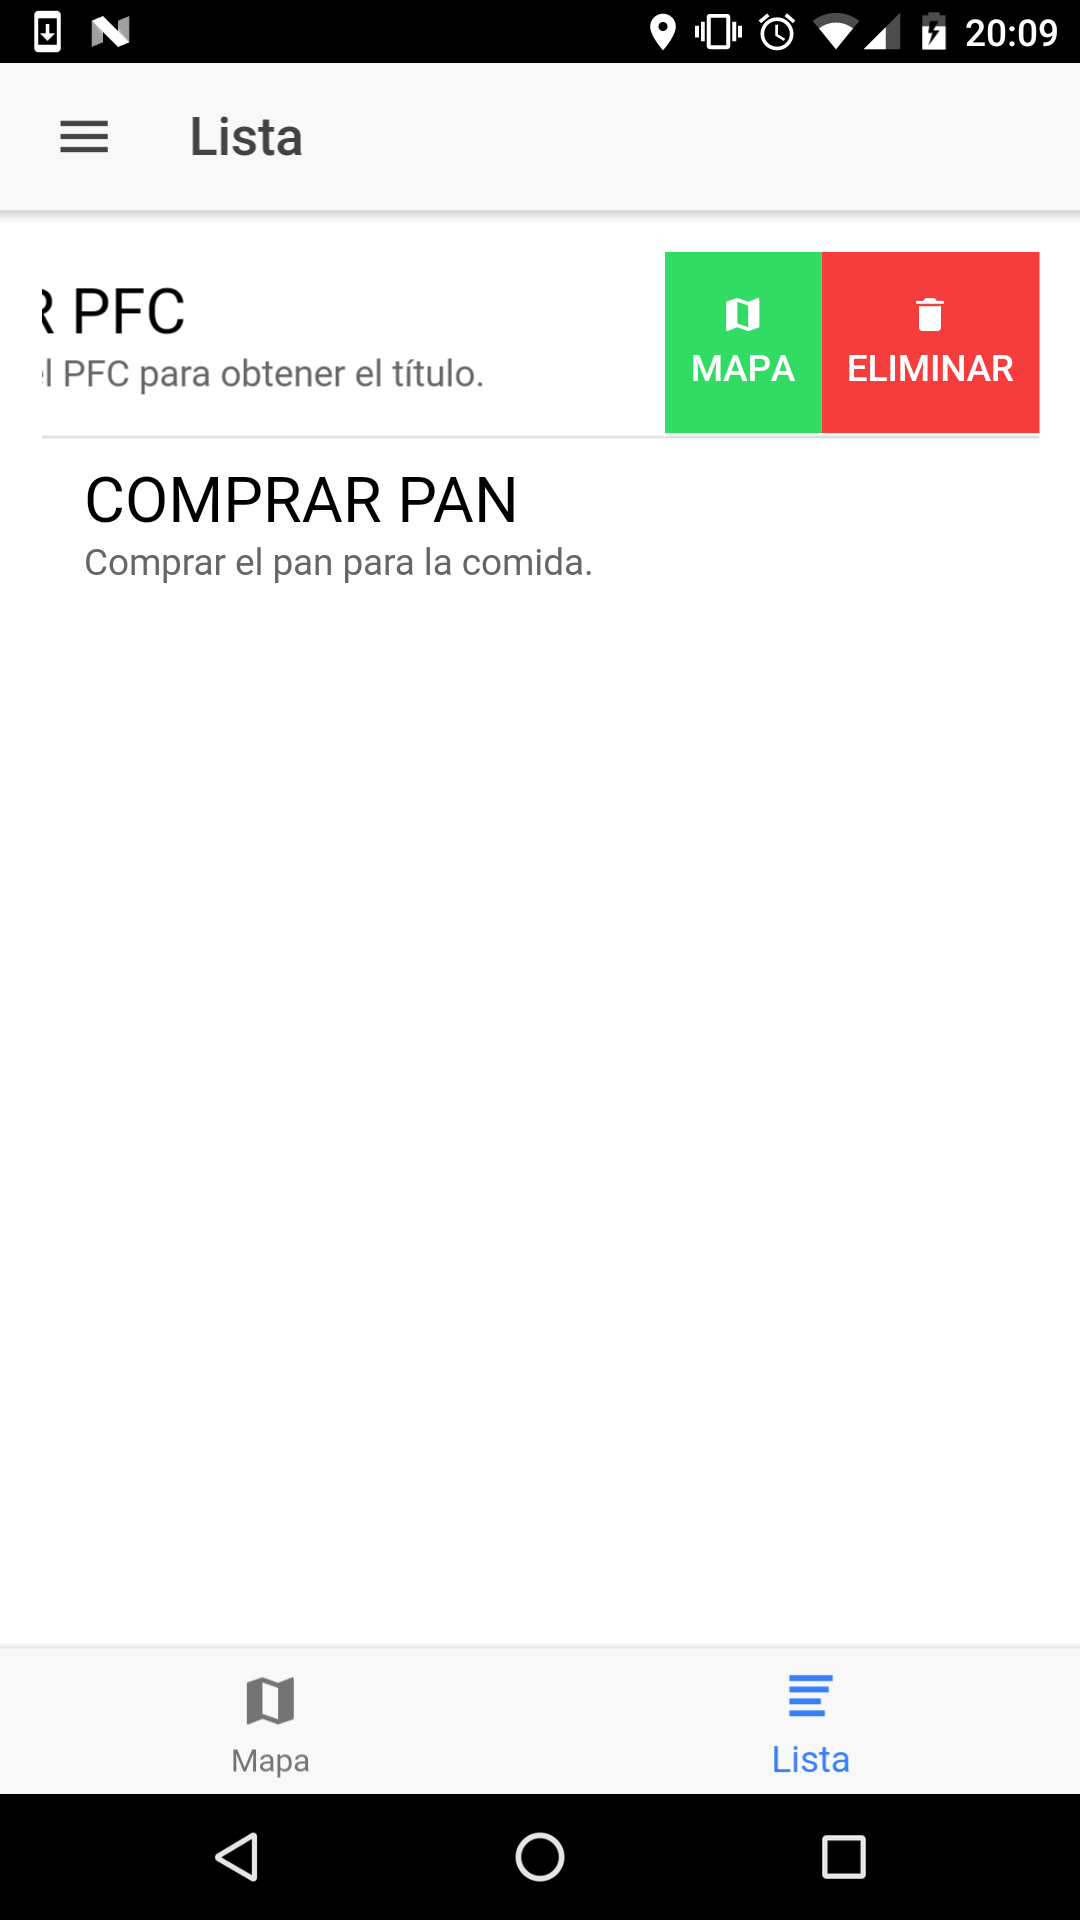
\includegraphics[width=0.4\textwidth]{Figures/ch2/ReminderMap/preview_list}
    \caption{Aquí vemos la lista de recordatorios, sobre los que podremos interactuar.}
\end{figure}

Los recordatorios quedarán almacenados de manera persistente en la \gls{BBDD} que implementa el sistema operativo, así, la información no se perderá al cerrar la aplicación ni al apagar el dispositivo.

Y como objetivo último de la aplicación, se notificará al usuario de que cerca de la zona en la que se encuentra, tiene registrado un recordatorio. Dicha notificación  se activará al entrar dentro del área de influencia de este:

\begin{figure}[H]
\centering
    \centering
        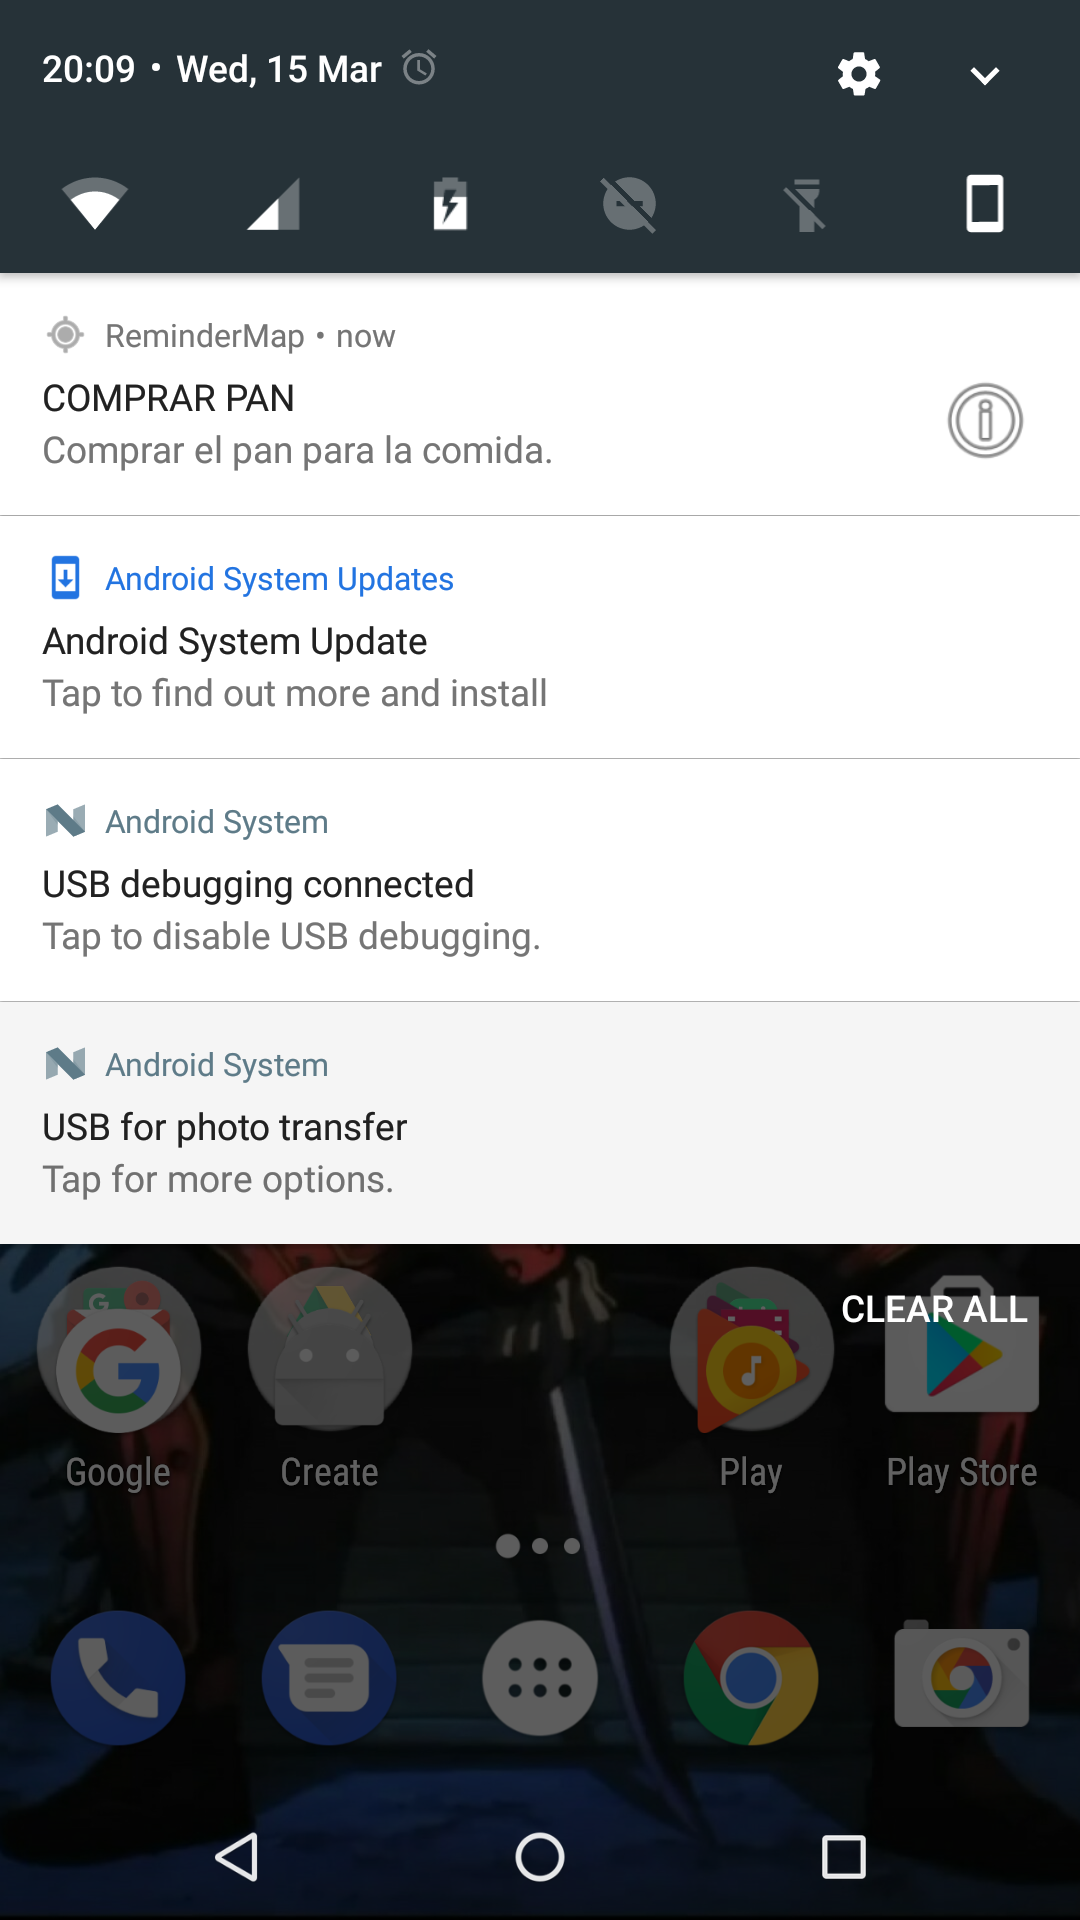
\includegraphics[width=0.4\textwidth]{Figures/ch2/ReminderMap/preview_alert}
    \caption{La notificación aparece aunque no este abierta la aplicación.}
\end{figure}

Para el desarrollo de esta aplicación se vamos a usar algunos módulos de Ionic Native. Como ya se vio en el apartado dedicado a \nameref{subsec:IonicNative}, se trata de un conjunto de envoltorios sobre algunos de los plugins con los que cuenta Cordova facilitando así su uso desde nuestro código escrito en TypeScript.

Entre todos los plugins disponibles, vamos a usar los siguientes:

\begin{enumerate}
  \item Google Maps\footnote{\url{https://ionicframework.com/docs/native/google\-maps/}}: Nos permitirá manejar de manera sencilla datos geográficos y visualizarlo sobre un mapa, crear y manipular estos mapas, acceder a los datos de geolocalización del dispositivo, \ldots para ello utiliza el SDK nativo de Google Maps.
  \item GeoFence\footnote{\url{https://ionicframework.com/docs/native/geofence/}}: También relacionado con la localización, pero implementado en un plugin diferente al anterior, nos permite crear alertas para cuando el dispositivo entre dentro de una zona geográfica definida. Estas alertas se mantienen incluso con la aplicación apagada.
  \item SQLite\footnote{\url{https://ionicframework.com/docs/native/sqlite/}}: Nos permite acceder a la \gls{BBDD} del dispositivo pudiendo hacer que nuestros datos sean persistentes mediante consultas \gls{SQL}
\end{enumerate}

Además, vamos a aprovechar esta práctica para ver como hacer uso de dos componentes de Ionic2 que son los \emph{tabs o pestañas} y el \emph{sidemenu o menú lateral}. Ambos componentes son muy utilizados en aplicaciones de todo tipo donde se quiere facilitar al usuario la navegación entre las diferentes páginas que la componen.

\subsubsection{Análisis funcional}

En esta aplicación se van a usar varios elementos como varias páginas, servicios, modelos de datos, plugins de Cordova, \ldot por lo que es interesante realizar un análisis funcional para tener una visión de los elementos que compondrán la aplicación y como interactúan entre ellos.

\begin{figure}[H]
\centering
    \centering
        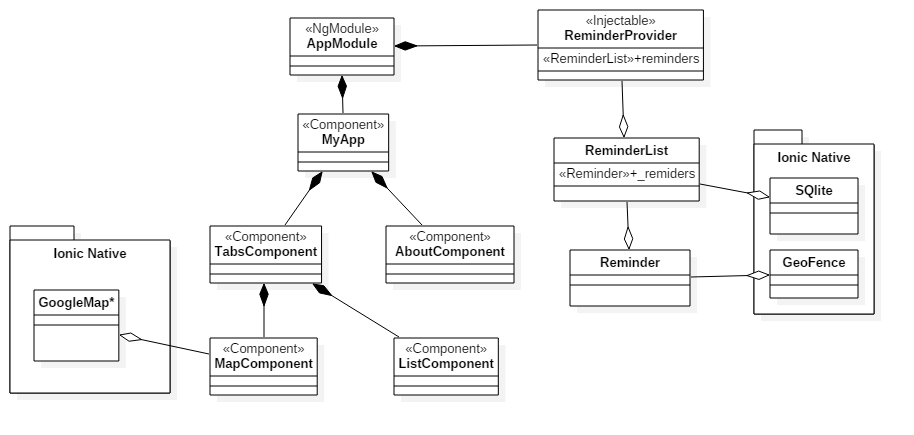
\includegraphics[width=0.8\textwidth]{Figures/ch2/ReminderMap/class_diagram}
    \caption{Diagrama de clases.}
\end{figure}

En el diagrama podemos ver como de nuestro módulo único parten las diferentes páginas de la aplicación. En primer lugar encontramos la página \emph{MyApp}, de la cual cuelgan todas las demás. \emph{MyApp} contendrá el menú lateral y desde el que se accederá a las páginas \emph{TabsComponent} y \emph{AboutComponent}. A su vez, \emph{TabsComponent} actuará de contenedor para \emph{MapComponent} y \emph{ListComponent}.

Por otro lado tenemos la clase \emph{Reminder}, que actuará como modelo y representará un recordatorio. Por encima de esta clase, se encuentra \emph{ReminderList}, que actuara como \emph{manager}, facilitando el manejo de los recordatorios y de la comunicación con la \gls{BBDD}.

También existirá un \emph{provider} que se usará para compartir inicializar un \emph{ReminderList} y que pueda ser compartido por todos los componentes de nuestra aplicación que lo necesiten, en nuestro caso, los componentes \emph{MapComponent} y \emph{ListComponent}. Esto se consigue utilizando el \emph{Dependency Injector} de Angular (ver \ref{sec:angular}).

Por último podemos ver el uso de los plugins de Ionic Native, comentados en la introducción, por parte de algunas de las clases.

\subsubsection{Estructura de las páginas}

En primer lugar vamos a crear las paginas de la aplicación y la navegación entre ellas. El aspecto que queremos tener en nuestra aplicación, y la navegación entre páginas se puede ver de manera gráfica en el siguiente esquema.

\begin{figure}[H]
\centering
    \centering
        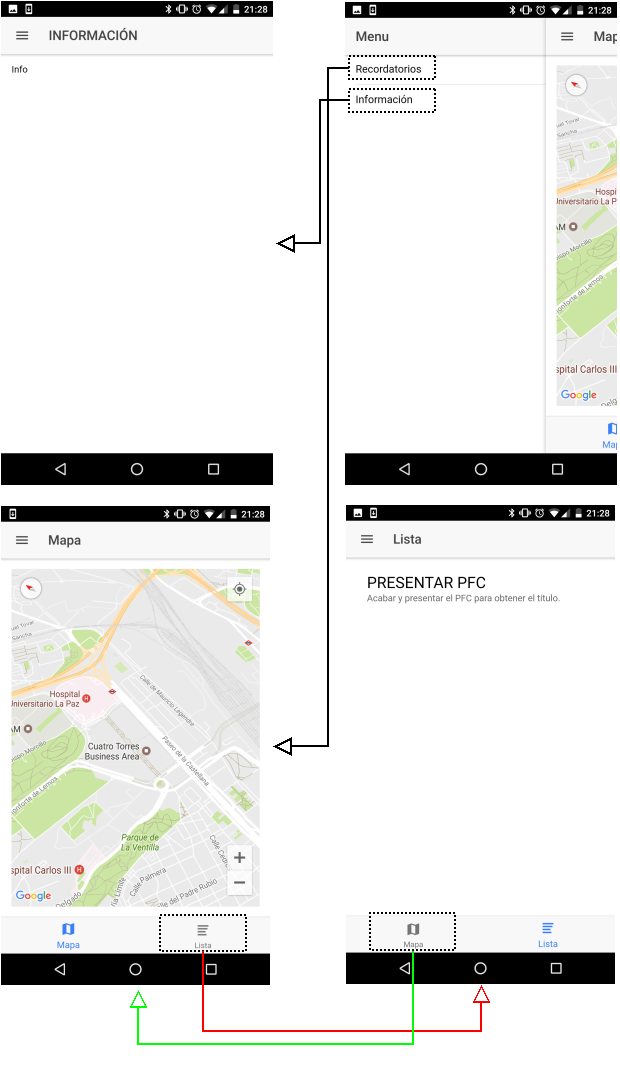
\includegraphics[height=0.7\textheight]{Figures/ch2/ReminderMap/mockup}
    \caption{Mockup de la aplicación. Podemos ver los enlaces entre páginas y los menús desde las que se acceden.}
\end{figure}

Necesitaremos implementar cuatro páginas diferentes para nuestra aplicación:

\begin{enumerate}
  \item Un una de las páginas se colocarán la barra de \emph{tabs} en la parte inferior. Además, deberá servir de contenedor para las siguientes dos páginas.
  \item Una página mostrará el mapa y que irá contenida en la anterior.
  \item Similar a la anterior, necesitaremos otra página para mostrar la información pero en formato de lista y también contenida en la primera.
  \item Una última página, esta vez dependiente de la página de \emph{tabs}, para mostrar la información sobre la aplicación.
\end{enumerate}

A su vez, como ocurre en todos los proyectos, estas páginas estarán contenidas dentro del componente padre de la aplicación, \emph{app}, y que será donde se implementará el menú lateral.

Vamos a empezar, pero en esta ocasión, en vez de usar un \emph{starter} vacío como era \emph{blank}, vamos a utilizar uno que ya implementa un menú lateral y al que iremos añadiendo nuestra páginas. Este \emph{starter} lo podemos encontrar en el market de Ionic2 y nos va a proporcionar la base para empezar una aplicación que cuente con un menú lateral. He aquí la importancia de revisar este market antes de ponerse a desarrollar por si podemos aprovechar lo ya desarrollado por otra persona.

Iniciamos nuestro proyecto con el siguiente comando, en el que podemos ver que el nombre del \emph{starter} a utilizar es \textbf{sidemenu}:

\begin{lstlisting}[language=bash]
  # ionic start ReminderMap sidemenu --v2
\end{lstlisting}

Si ejecutamos el proyecto tal cual, veremos que podemos abrir un menú lateral en el que aparecen dos páginas, a las que podemos acceder pulsando sobre ellas.

\begin{figure}[H]
\centering
    \centering
        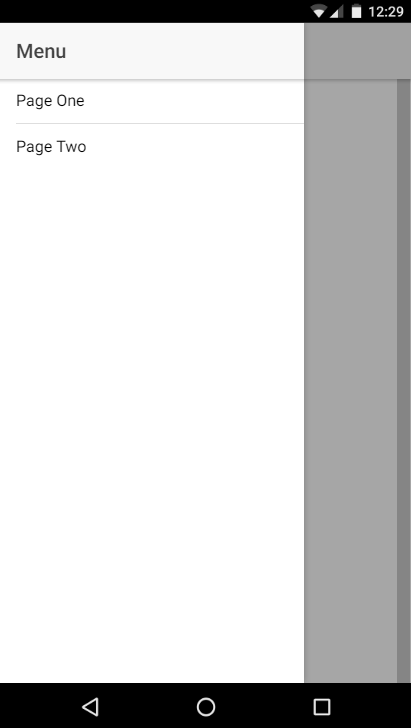
\includegraphics[width=0.4\textwidth]{Figures/ch2/ReminderMap/sidemenu_starter_serve}
    \caption{Menú lateral que nos proporciona la plantilla sidemenu.}
\end{figure}

Estas páginas que vemos se crean por defecto. Pueden ser editadas y añadir así nuestro contenido o, como vamos a hacer nosotros, podemos eliminarlas y crear las nuestras desde cero. Generaremos nuestras páginas utilizando Ionic CLI, consiguiendo que nuestras páginas tengan la estructura necesaria de ficheros usando un único comando. Las páginas a crear son las comentadas unos párrafos atrás:

\begin{lstlisting}[language=bash]
  # ionic generate page tabs
  # ionic generate page map
  # ionic generate page list
  # ionic generate page about
\end{lstlisting}

Empezaremos modificando el menú lateral para que muestre la páginas \emph{tabs} y \emph{about}. A continuación, añadiremos el componente de Ionic \textbf{ion-tabs} a la página \emph{tabs} y enlazaremos las páginas \emph{maps} y \emph{list} a este componente.

Editamos el archivo \emph{/app/app.html}, que actúa como página padre de la aplicación. Aquí vemos la primera implementación que añade el \emph{starter} \textbf{sidemenu}.

\begin{lstlisting}[style=htmlcssjs,frame=tlrb,xleftmargin={0.2cm}]
  <ion-menu [content]="content" >
    <ion-header>
      <ion-toolbar>
        <ion-title>Menu</ion-title>
      </ion-toolbar>
    </ion-header>

    <ion-content>
      <ion-list>
        <button menuClose ion-item *ngFor="let p of pages" (click)="openPage(p)" >
          {{p.title}}
        </button>
      </ion-list>
    </ion-content>

  </ion-menu>

  <!-- Disable swipe-to-go-back because it's poor UX to combine STGB with side menus -->
  <ion-nav [root]="rootPage" #content swipeBackEnabled="false" ></ion-nav>
\end{lstlisting}

Encontramos el componente \textbf{ion-menu}, el cual se inicia con los valores que encuentra dentro de la propiedad \emph{pages}, que pertenece al componente \emph{MyApp} que se encuentra dentro del fichero \emph{app.component.ts}. Lo abrimos y vemos que se trata de un diccionario en el que se indica el título del botón y la página a la que hace referencia. También vemos la función \textbf{openPage}, que es llamada desde los botones del menú (función asignada al evento \emph{click}) y que se encarga de abrir la página correspondiente. Cambiamos pues este diccionario para introducir nuestras páginas de la siguiente forma:

\begin{lstlisting}[style=htmlcssjs,frame=tlrb,xleftmargin={0.2cm}]
    this.pages = [
      { title: 'Recordatorios', component: TabsPage },
      { title: 'Información', component: AboutPage }
    ];
\end{lstlisting}

También cambiamos la variable \textbf{rootPage}, que define la página de inicio, por \textbf{TabsPage}. No nos debemos olvidar de importar nuestras páginas.

Como estamos usando páginas creadas por nosotros, tendremos que declararlas y añadirlas como \emph{entryComponents} \footnote{\url{https://angular.io/docs/ts/latest/cookbook/ngmodule-faq.html}}. Estos cambios se han de realizar en la definición del \emph{ngModule}, en el fichero \emph{app.module.ts}. Eliminamos las páginas que venían definidas en el \emph{starter} y añadimos nuestras  propias páginas.

\begin{lstlisting}[style=htmlcssjs,frame=tlrb,xleftmargin={0.2cm}]
  declarations: [
      MyApp,
      AboutPage,
      TabsPage,
      MapPage,
      ListPage
    ],
    ...
    entryComponents: [
      MyApp,
      AboutPage,
      TabsPage,
      MapPage,
      ListPage
    ]
\end{lstlisting}

Ya tenemos creado nuestro menú lateral con el que acceder a nuestra página principal y a la de información. Ahora vamos a añadir el componente \textbf{ion-tabs} a nuestra página \emph{tabs.html}. La editamos con el siguiente código:

\begin{lstlisting}[style=htmlcssjs,frame=tlrb,xleftmargin={0.2cm}]
  <ion-tabs selectedIndex="0" >
    <ion-tab [root]="mapTabRoot" tabTitle="Mapa" tabIcon="map" ></ion-tab>
    <ion-tab [root]="listTabRoot" tabTitle="Lista" tabIcon="list" ></ion-tab>
  </ion-tabs>
\end{lstlisting}

Como se observa, se han añadido dos \emph{tabs} a los que se les ha definido un texto (atributo \textbf{tabTitle}) y un icono (de los disponibles en la fuente Ionicons y definido por el atributo \textbf{tabTitle}). Con el atributo \textbf{[root]} se indica la página que se debe mostrar al seleccionar esa pestaña. El parámetro que se indica en este atributo debe estar definido como propiedad en el componente de la página, en \emph{TabComponent}:

\begin{lstlisting}[style=htmlcssjs,frame=tlrb,xleftmargin={0.2cm}]
  @Component({
    templateUrl: 'tabs.html'
  })
  export class TabsPage {
    mapTabRoot: any = MapPage;
    listTabRoot: any = ListPage;

    constructor() {}
  }
\end{lstlisting}

Por último, y para acabar con la estructura de páginas que tendrá la aplicación, añadiremos cabeceras que contengan a cada una de las páginas con un título que las identifique junto a un botón con el que abrir el menú lateral. La cabecera para todas ellas sería así:

\begin{lstlisting}[style=htmlcssjs,frame=tlrb,xleftmargin={0.2cm}]
  <ion-header>
    <ion-navbar>
      <button ion-button menuToggle>
        <ion-icon name="menu" ></ion-icon>
      </button>
      <ion-title>INFORMACIÓN</ion-title>
    </ion-navbar>
  </ion-header>
\end{lstlisting}

Esta cabecera deberá ir en todas las páginas menos en la pagina \emph{tabs}, ya que está actúa de contenedor de páginas que poseen su propia cabecera.

\subsubsection{Instalando los plugins necesarios}

Antes de empezar a implementar la lógica, vamos a instalar los plugins que hemos enumerado y que necesitaremos para nuestra aplicación. Los plugins se pueden instalar utilizando Ionic CLI. Se recomienda añadir en primer lugar las plataformas objetivo al proyecto, y a continuación, instalar los plugins. Empecemos:

\begin{lstlisting}[language=bash]
  # ionic platform add android
\end{lstlisting}

Seguimos con un plugin usado para gestionar la política de acceso a páginas desde la aplicación. No lo usaremos directamente, pero es necesario para que nuestro mapa funcione.

\begin{lstlisting}[language=bash]
  # ionic plugin add cordova-plugin-whitelist
\end{lstlisting}

El caso del plugin de Google Maps tiene la particularidad de que hay que indicar que API KEY del servicio debe utilizar ya en el momento de la instalación del módulo. En el anexo \nameref{ch:google_api} podemos ver como conseguir esta API KEY. En el momento de escribir este documento, el plugin se encuentra en la versión 1.4, aunque la versión 2 ya está desarrollada y en fase beta. Vamos a usar la versión 1.4, la cual indicaremos en el comando para asegurarnos de que es la que se instala.

\begin{lstlisting}[language=bash]
  # ionic plugin add cordova-plugin-googlemaps@1.4 --variable API_KEY_FOR_ANDROID=MY_API_KEY
\end{lstlisting}

El resto de plugin no tienen ninguna peculiaridad a destacar.

\begin{lstlisting}[language=bash]
  # ionic plugin add cordova-sqlite-storage
  # ionic plugin add cordova-plugin-geofence
\end{lstlisting}

Cabe destacar la facilidad que ofrece no Ionic a la hora de añadir nuevos plugin a cualquier aplicación.

\subsubsection{Implementación del modelo de datos y la persistencia}

Como hemos visto en el análisis, nuestra aplicación va a contar con una clase que actúe de modelo y que contenga la información de un recordatorio. Ya que la aplicación podrá manejar varios recordatorios, y estos deberán ser guardados en la \gls{BBDD} del dispositivos y poder ser recuperados de ella, se implementará una clase que abstraiga de estas tareas al resto de clases.

\tipbox{Como ocurre en muchos otros lenguajes, existen módulos para Ionic2 que implementan el modelo \gls{ORM}\footnote{\url{https://github.com/BradyLiles/ionic-orm}}. Este modelo se basa en el mapeado de las tablas de una \gls{BBDD} en entidades que simplifiquen las tareas básicas de acceso a esas tablas.}

Vamos a empezar definiendo la clase \emph{Reminder} que actuara de modelo para nuestros recordatorio.

\begin{lstlisting}[style=htmlcssjs,frame=tlrb,xleftmargin={0.2cm}]
  export class Reminder {
    private _id: number;
    private _name: string;
    private _description: string;
    private _lat: number;
    private _lng: number;

    constructor(name: string, description: string,
    latLng: GoogleMapsLatLng | Array<number>, id: number=null) {
      this._id = id;
      this.name = name;
      this.description = description;
      if (latLng instanceof Array) {
        this._lat = latLng[0];
        this._lng = latLng[1];
      } else {
        this._lat = latLng['lat'];
        this._lng = latLng['lng'];
      }
    }

    get id(): number { return this._id;
    }

    get name(): string { return this._name;
    }

    set name(name: string) { this._name = name.substr(0, 16);
    }

    get description(): string { return this._description;
    }

    set description(description: string) {
      this._description = description.substr(0, 512);
    }

    get latLng(): GoogleMapsLatLng {
      return new GoogleMapsLatLng(this._lat, this._lng);
    }

    set latLng(latLng: GoogleMapsLatLng ) {
      this._lat = latLng['lat'];
      this._lng = latLng['lng'];
    }
  }
\end{lstlisting}

Se puede observar que se han declarado las variables privadas y se ha decidido implementar sus métodos \emph{getter} y \emph{setter}. Con esto se consigue tener control sobre asignación de valores a estas variables, como por ejemplo, la longitud del nombre o la imposibilidad de modificar el id. Por otro lado, la localización se define como dos variables, una para la latitud y otra para la longitud, pero a la hora de querer modificar o recuperar esta localización, se usa un objeto de tipo \emph{GoogleMapsLatLng}. Se ha decido hacer esto así ya que este tipo de objetos es el que usa el plugin de Google Map para representar una coordenada geográfica. Pero, ¿y por qué no definirlo también así en nuestro modelo?. La razón es que nuestro modelo va a ser almacenado dentro de una \gls{BBDD}, y no podremos guardar directamente en ella el objeto \emph{GoogleMapsLatLng} directamente, sino que necesitaremos serializarlo o descomponerlo en elementos de tipo básico. Además, no siempre se puede usar \emph{GoogleMapsLatLng} para definir una coordenada, como ya veremos a la hora de usar \emph{GeoFence}.

Implementamos también nuestro \emph{ReminderList}, que tendrá como variable un \emph{Array} de elementos de tipo \emph{Reminder}, el cuál será privado y accedido a través de la función \emph{all()}:

\begin{lstlisting}[style=htmlcssjs,frame=tlrb,xleftmargin={0.2cm}]
  export class ReminderList {
    private _reminders: Array<Reminder>;

    constructor(public events: Events) {}

    all(): Array<Reminder> { return this._reminders;
    }
  }
\end{lstlisting}

Con estas dos clases ya definidas, vamos a ir añadiéndoles funcionalidades. Para empezar, añadiremos persistencia a los datos, es decir, crearemos los métodos necesarios para poder leer y escribir en la \gls{BBDD} del dispositivo. Tendremos que importar la clase \textbf{SQLite} desde el paquete \textbf{ionic-native}.

Para utilizar una \gls{BBDD}, debemos instanciar un objeto de esta clase con el cual podremos abrir una \gls{BBDD} usando el método \textbf{openDatabase} y ejecutar queries sobre ella con el método \textbf{executeSql}. Ambos métodos nos devolverán promesas, en las cuales indicaremos la acción a realizar en función de si la operación haya ido bien o mal. Empecemos viendo como quedaría el constructor de nuestra clase \emph{ReminderList}.

\begin{lstlisting}[style=htmlcssjs,frame=tlrb,xleftmargin={0.2cm}]
  export class ReminderList {
    private _db: SQLite;
    // RESTO DE VARIABLES

    constructor(public events: Events) {
      this._db = new SQLite();
      this._db.openDatabase({
        name: 'reminder.db',
        location: 'default'
      }).then(() => {
        this._db.executeSql('CREATE TABLE IF NOT EXISTS reminders (id INTEGER PRIMARY KEY,' +
          'name VARCHAR(16), description VARCHAR(512), lat FLOAT, lng FLOAT)', []
        ).then((data) => {
            this.refresh();
        }, (err) => {
          console.error('Unable to execute sql: ', err);
        });
      }, (err) => {
        console.error('Unable to open database: ', err);
      });
    }
    // RESTO DE MÉTODOS
  }
\end{lstlisting}

En primer lugar se instancia un objeto \emph{SQLite} el cual asignamos a una propiedad privada de \emph{ReminderList}. Abrimos la \gls{BBDD} con el ya mencionado método \textbf{openDatabase}, al cual se le indica el nombre de la \gls{BBDD} y la localización (usaremos \emph{default}). Si la \gls{BBDD} se ha abierto sin problemas, podremos ejecutar nuestra primera query. Con esta primera query crearemos la tabla en la que se escribirá la información de los recordatorios, solo si no existe ya. Se han definido las columnas acorde al tipo de dato que van a almacenar, además, se ha definido la columna \emph{id} como \textbf{PRIMARY KEY}. Si todo ha ido según se espera, podremos llamar al método \emph{refresh()}, el cual poblará el \textbf{Array} \emph{\_reminder} con la información de la tabla. La definición de este método es la siguiente:

\begin{lstlisting}[style=htmlcssjs,frame=tlrb,xleftmargin={0.2cm}]
  onUpdate: EventEmitter<Array<Reminder>> = new EventEmitter();

  refresh() {
    this._reminders = [];
    this._db.executeSql('SELECT * FROM reminders', []).then(
      (data) => {
          for (let i = 0; i < data.rows.length; i++) {
            let item = data.rows.item(i);
            this._reminders.push(new Reminder(item.name, item.description,
              [item.lat, item.lng], item.id))
          }
          this.onUpdate.emit(this._reminders);
      }, (err) => {
        console.error('Unable to execute sql: ', err);
      }
    )
  }
\end{lstlisting}

En este método se asigna un array vacío a la variable \emph{\_reminder}. Acto seguido, se ejecuta una query \gls{SQL} para recuperar toda la información de la tabla. Si todo ha ido bien, las filas que devuelve la query son mapeados en un \gls{JSON} que se pasa como parámetro a la primera función que se indica en la promesa que devuelve \textbf{executeSql}. Recorremos estas filas y vamos instanciando nuevos recordatorios que añadimos a nuestro \textbf{Array}. También vamos a añadir a la clase \emph{ReminderList} un \textbf{EventEmitter}. A este emisor de eventos podrán subscribirse el resto de clases para ser notificadas, en este caso, de que se han actualizado la lista de recordatorios. Veremos como usarlo cuando implementemos el \emph{MapsComponent}. Gracias a estos eventos, podemos comunicar diferentes clases dentro de nuestra aplicación de manera sencilla.

Ya tenemos como recuperar los recordatorios desde la \gls{BBDD}, nos falta poder añadir nuevos y eliminar los ya creados. Esto lo haremos co dos nuevos métodos en \emph{ReminderList}:

\begin{lstlisting}[style=htmlcssjs,frame=tlrb,xleftmargin={0.2cm}]
  addReminder(name: string, description: string, latLng: GoogleMapsLatLng) {
    let rem = new Reminder(name, description, latLng); // Se llama al constructor sin pasarle un id como parametro
    rem.save(this._db);
    this.refresh();

    return rem;
  }

  removeReminder(rem: Reminder) {
    rem.remove(this._db);
    this.refresh()

    return rem;
  }
\end{lstlisting}

Curioso. En ninguno de los métodos se hace una consulta a la \gls{BBDD}, si no que se invoca a unos métodos pertenecientes a la clase \emph{Reminder} (veremos a continuación la implementación de estos métodos). Pero, ¿por qué?. Si pensamos que las acciones tanto de añadir como de eliminar solo afectan al recordatorio en cuestión, resulta comprensible que esta puedan ser llevadas a cabo por el recordatorio mismo. Además, si otra clase distinta a \emph{ReminderList} quisiera guardar un recordatorio en la BBDD, no necesitaría implementar la lógica para ello en dicha clase, solo tendría que usar las facilidades que implementa el propio \emph{Reminder}. Cabe destacar que a la hora de instanciar el nuevo objeto \emph{Reminder} en el método \emph{addReminder}, no se le pasa el valor del ID. Esto se debe a que esta columna fue definida como índice de la tabla y será generado por la \gls{BBDD} como veremos a continuación.

Ahora solo nos queda implementar los métodos de la clase \emph{Reminder} de los que hablábamos antes:

\begin{lstlisting}[style=htmlcssjs,frame=tlrb,xleftmargin={0.2cm}]
  save(db) {
    db.executeSql('INSERT INTO reminders (name, description, lat, lng) VALUES (?, ?, ?, ?)',
      [this._name, this._description, this._lat, this._lng]).then(
        (data) => { this._id = data.insertId; // El ID devuelto por la \gls{BBDD}, se asigna al campo _id del recordatorio.
        }, (err) => { console.error('Unable to execute sql: ', err);
        }
      )
    return this;
  }

  remove(db) {
    if (!this._id) { return this;
    }
    db.executeSql('DELETE FROM reminders WHERE id = ?', [this._id]).then(
        (data) => {
          this._id = null;
        }, (err) => { console.error('Unable to execute sql: ', err);
        }
      )
    return this;
  }
\end{lstlisting}

Como ya comentábamos, el ID se asigna cuando se añade el recordatorio a la \gls{BBDD}, siendo este ID pasado como campo dentro del \gls{JSON} de datos que envía la promesa en caso de que todo haya ido bien. Por su parte, el método de borrado comprueba antes de realizar la consulta \emph{SQL} que el objeto tiene asignado un ID, ya que usara este ID para identificar el recordatorio dentro de la tabla de la \gls{BBDD}.

Podemos ver que, aunque instanciemos un objeto de la clase \emph{Reminder}, esto no quiere decir que ya la hayamos almacenado en la \gls{BBDD}. Será necesario llamar a su método \emph{save} para ello.

\tipbox{Pensemos en el caso de que queramos acceder a la tabla de recordatorios no solo desde la clase \emph{ReminderList}, si no también desde otras clases. Esto obligaría duplicar el código que se utiliza para crear la tabla y para leerla. En ese caso sería interesante que toda esta lógica se encontrara también dentro de \emph{Reminder} en forma de métodos estáticos. En nuestra aplicación no nos será necesario, por lo que se ha decidido dejar esa lógica dentro de \emph{RemiderList}}

\tipbox{En este caso, al leer los recordatorios desde la base da datos, se hace una lectura de todos sin aplicar ningún filtro. Pero, ¿y si queremos filtrar por alguno de sus campos?¿y si quisiéramos realizar búsquedas sobre el campo \emph{nombre} del recordatorio?. En este caso podríamos o bien, leer recuperar todos los recordatorios desde la \gls{BBDD} y luego descartarlos utilizando JavaScript, o se puede directamente añadir condiciones mediante la clausula WHERE a la query \emph{SQL} para solo recuperar de la \gls{BBDD} los registros deseados. Esta segunda opción es de lejos la más recomendable ya que se evita por un lado tener que recuperar información de la \gls{BBDD} que luego va a ser descartada y además, uno de los puntos fuertes de las \gls{BBDD} es precisamente aplicar filtros, por lo que será mas rápido.}

\subsubsection{ReminderProvider}

Una vez que tenemos implementadas las clases que nos permitirán manejar los recordatorios, debemos pensar como interactuarán los componentes de la aplicación con ellas.

Tenemos dos componentes que necesitarán acceder a la lista de recordatorios, que son \emph{MapComponent} y \emph{ListComponent}. Podríamos hacer que cada uno de ellos instanciara un objeto de la clase \emph{ReminderList}, pero sería duplicar recursos y peticiones. Para solventar esto crearemos un \emph{provider}, que se trata una clase \emph{singleton} (solo se instancia una vez) y que estará disponible para ambos componentes gracias a \gls{DI}. Este \emph{provider}, al igual que ocurría con las páginas, puede ser generado utilizando Ionic CLI:

\begin{lstlisting}[language=bash]
  # ionic generate provider Reminder
\end{lstlisting}

Sobrescribimos el contenido:

\begin{lstlisting}[style=htmlcssjs,frame=tlrb,xleftmargin={0.2cm}]
  @Injectable()
  export class Reminder {
    private _reminders: ReminderList;

    constructor() {
      this._reminders = new ReminderList();
    }

    get reminders(): Array<Reminder> {
      return this._reminders.reminders;
    }
  }
\end{lstlisting}

Y no nos olvidemos de registrarlo en el \emph{AppModule}:

\begin{lstlisting}[style=htmlcssjs,frame=tlrb,xleftmargin={0.2cm}]
  @NgModule({
    // Resto de declaraciones
    providers: [{provide: ErrorHandler, useClass: IonicErrorHandler},
                {provide: ReminderProvider, useClass: ReminderProvider}]
  })
  export class AppModule {}
\end{lstlisting}

Como se puede ver, se trata de una clase muy simple y que nos solventa el hecho de tener que compartir un mismo objeto entre diferentes clases.

\subsubsection{El mapa}

Una vez que contamos con los elementos necesarios para manejar los recordatorios dentro de nuestra aplicación, llega el momento de implementar la visualización de estos recordatorios. Empezaremos por la página del mapa. Para crear este mapa, necesitaremos un contenedor, dentro del cual, el plugin de Google Maps se encargará de ``dibujar'' el mapa. Este contenedor no será más que un \textbf{div} dentro del \gls{HTML} de la página.

\noindent
\begin{minipage}[t]{.48\textwidth}
{\begin{lstlisting}[style=htmlcssjs,frame=tlrb,xleftmargin={0.2cm}]
<ion-content padding>
  <div id="map" ></div>
</ion-content>
\end{lstlisting}}
\end{minipage}\hfill
\noindent
\begin{minipage}[t]{.48\textwidth}
{\begin{lstlisting}[style=htmlcssjs,frame=tlrb,xleftmargin={0.2cm}]
page-map {
  #map {
    width: 100%;
    height: 100%;
  }
}
\end{lstlisting}}
\end{minipage}

Ahora abrimos el \emph{component} \emph{MapPage}, donde crearemos un método, \emph{loadMap} en el que iniciaremos nuestro mapa.

\begin{lstlisting}[style=htmlcssjs,frame=tlrb,xleftmargin={0.2cm}]
  loadMap() {
    let location = new GoogleMapsLatLng(40.4893538, -3.6827461);
    this.map = new GoogleMap('map', {
      'backgroundColor': 'white',
      'controls': {
        'compass': true,
        'myLocationButton': true,
        'zoom': true
      },
      'gestures': {
        'scroll': true,
        'tilt': true,
        'rotate': true,
        'zoom': true
      },
      'camera': {
        'latLng': location,
        'zoom': 15
      }
    });

    this.map.on(GoogleMapsEvent.MAP_READY).subscribe(() => {
        console.log('Map is ready!');
    });
  }
\end{lstlisting}

Vemos como para crear un mapa, debemos instanciar la clase GoogleMap, contenida en \textbf{ionic-native}, cuyo constructor espera el id del \textbf{div} que usará para dibujar el mapa, y un \gls{JSON} con la configuración del mapa (posición inicial, botones, gestos permitidos, \ldots)\footnote{\url{https://github.com/mapsplugin/cordova-plugin-googlemaps-doc/blob/master/v1.4.0/class/Map/README.md}}. Asignaremos este objeto a la variable \emph{map} del componente para poder hacer uso de ella más adelante. También subscribiremos una función al evento \emph{MAP\_READY}, el cual se dispara cuando el mapa está listo. De momento solo haremos que se imprima un mensaje en consola cuando esto ocurra, más adelante, iremos poblando este método.

Llegados a este punto, y antes de añadir más código, se recomienda ejecutar nuestra aplicación y comprobar si el mapa funciona correctamente. No podremos usar para esto el servidor de Ionic (\emph{ionic serve}) y acceder a él a través del navegador, ya que el plugin Cordova Google Maps requiere que sea ejecutado sobre un dispositivo, ya sea emulado o real.

\warningbox{Nuestra aplicación requerirá de permisos para poder acceder al \gls{GPS}. Debemos asegurarnos, una vez instalada en el terminal, de que cuenta con ellos.}

\warningbox{En Android encontramos nos encontramos con la aplicación Google Play Services\footnote{\url{https://developers.google.com/android/guides/overview}}, a través de la cual, el resto de aplicaciones pueden acceder a diferentes servicios, en el caso de nuestra aplicación, a Google Maps. La razón de porque Android hace esto así es la de asegurarse de que todas las aplicaciones que ejecuta el dispositivo hacen uso de unas mismas librerías a la hora de utilizar sus servicios. Librería la cual puede mantener actualizada fácilmente ya que se trata de una aplicación como otra cualquiera.

Si después de añadir la plataforma Android a nuestro proyecto, abrimos el fichero \emph{/platforms/android/project.properties}, y vamos añadiendo los plugin, veremos como se añaden líneas como: \textbf{cordova.system.library.1=com.google.android.gms:play-services-location:9.8.0}. Esta línea indica que librería, dentro de Google Play Services se va a usar, así como la versión.
En el momento de desarrollar esta app y probar a ejecutarla, se producía un error al intentar construir el APK. Este error se debía a que el plugin Cordova Geofence añade la siguiente línea a \emph{project.properties} \textbf{cordova.system.library.1=com.google.android.gms:play-services-location:+}, haciendo que se utilizara la versión 10.2 de la librería. Cambiando esta versión por la 9.8.0 se pudo evitar el error y generar la APK}

Con el mapa ya funcionando, el siguiente paso será poder crear nuevos recordatorios desde él y poder visualizar los ya presentes en la \gls{BBDD}. En el siguiente diagrama de actividad se describe como será el proceso para crear un nuevo recordatorio.

\begin{figure}[H]
\centering
    \centering
        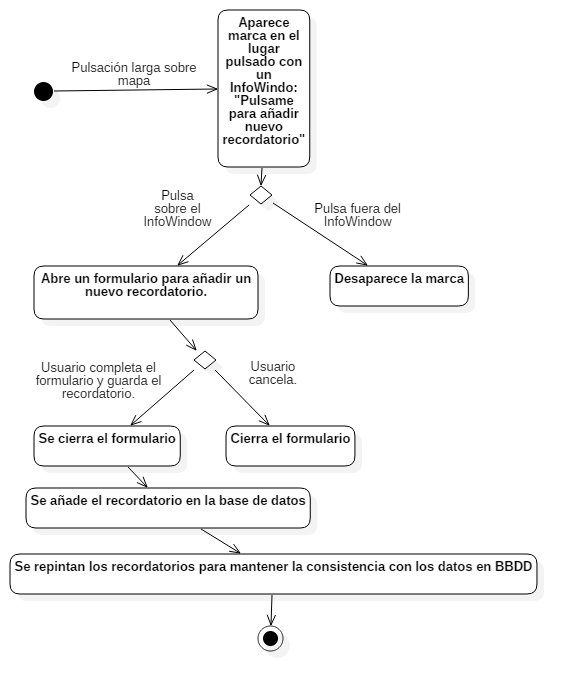
\includegraphics[width=0.8\textwidth]{Figures/ch2/ReminderMap/add_reminder_diagram}
    \caption{Diagrama de actividad que muestra la creación de un nuevo recordatorio.}
\end{figure}

Los elementos con los que el usuario interactuará durante el proceso (marca en el mapa, inforwindow, \ldots) son elementos que el propio framework pone a disposición del desarrollador, por lo que no tenemos que preocuparnos de implementarlos (diseñarlos, escribir el HTML, crear funciones que controlen la lógica, \ldots), lo cual supone un ahorro de tiempo considerable.

Modificaremos el código de nuestro \emph{MapComponent} de la siguiente manera:

\begin{lstlisting}[style=htmlcssjs,frame=tlrb,xleftmargin={0.2cm}]
  loadMap() {
    // RESTO DE LA FUNCIÓN

    this.map.on(GoogleMapsEvent.MAP_LONG_CLICK).subscribe((latLng) => {
      this.showAddNewReminderInfoWindow(latLng);
    });
  }

  showAddNewReminderInfoWindow(latLng: GoogleMapsLatLng) {
    let markerOptions: GoogleMapsMarkerOptions = {
      'position': latLng,
      // En las opciones de la marca, podemos configurar el infoWindow asociado a esta.
      'title': 'NUEVO RECORDATORIO'
      'snippet': "Click sobre mí si quieres añadir un nuevo recordatorio en esta localización.",
      'infoClick': (marker) => {
        // Se elimina la marca del mapa y se abre el formulario para añadir un nuevo recordatorio.
        marker.remove();
        this.showAddNewReminderPrompt(latLng);
      }
    };

    // Añadimos la marca al mapa, y cuando esté lista, hacemos que muestre en el infoWindow.
    this.map.addMarker(markerOptions).then((marker: GoogleMapsMarker) => {
      marker.showInfoWindow();
    });
  }

  showAddNewReminderPrompt (latLng: GoogleMapsLatLng) {
    // Deshabilitamos la interacción con el mapa
    this.map.setClickable( false )
    let prompt = this.alertCtrl.create({
      // Elegimos El mensaje que queremos que aparezca en nuestro formulario
      title: 'Nuevo recordatorio',
      message: "Se creará un nuevo recordatorio para la localización seleccionada.",
      // Configuramos los diferentes inputs que va a tener nuestro formulario indicando el texto que se mostrará y el nombre con el que será identificado este valor a la hora de devolver el los datos introducidos.
      inputs: [
        {
          name: 'name',
          placeholder: 'Nombre'
        },
        {
          name: 'description',
          placeholder: 'Descripción',
          type: 'text'
        },
      ],
      // También configuramos los botones que queremos que aparezcan, en este caso indicamos el texto del botón y la acción a realizar
      buttons: [
        {
          text: 'Cancelar',
          handler: data => { console.log('Cancel clicked');
          }
        },
        {
          text: 'Guardar',
          handler: data => {
            this.remindersProvider.reminders.addReminder(data['name'], data['description'], latLng);
          }
        }
      ]
    });
    // Hacemos que la iteración con el mapa se vuelva a habilitar cuando el formulario se cierre
    prompt.onDidDismiss(() => this.map.setClickable( true ));
    // Mostramos el formulario
    prompt.present();
  }
\end{lstlisting}

Se puede ver que se ha añadido al método \emph{loadMap()} una nueva instrucción para capturar el evento asociado a las pulsaciones largas sobre el mapa. Este evento lleva asociado las coordenadas sobre la que se ha pulsado. Cuando esto se produce, se ejecuta la función que hace que aparezca una marca sobre el mapa. Como comentaba antes, este elemento lo ofrece el propio framework, en este caso, a través del plugin de Google Maps. Para crearlo, se utiliza el método \emph{addMarker()} de nuestro mapa (que fue instanciado en el constructor), al cuál se le pasa un objeto de tipo \emph{GoogleMapsMarkerOptions} con la configuración de la marca y el InfoWindow asociado. Para ver más opciones, se puede consultar la documentación de este elemento en la página de Github \footnote{\url{https://github.com/mapsplugin/cordova\-plugin\-googlemaps/wiki/marker}}. El método \emph{addMarker()} devuelve una promesa, lo que nos permite ejecutar código en el momento en el que la marca esté lista. Vamos a aprovechar esta promesa para hacer que muestre el infoWindow asociado a la marca.

En caso de que el usuario pulse sobre el InfoWindow, se ejecutará el método \emph{showAddNewReminderPrompt()} que hará que aparezca un formulario con el cual añadir un nuevo recordatorio. Al igual que con las marcas, este formulario será implementado utilizando componentes que ofrece el Ionic. En este caso nos aprovecharemos del servicio de alertas, el cual no es más que un \emph{provider} que podemos inyectar desde el constructor y que permite la creación ventanas flotantes en nuestra aplicación. Para ello, solamente tenemos que llamar al método \emph{create()} del servicio de alertas pasandole la configuración que deseamos. En la documentación de Ionic podemos ver que parametros podemos configurar\footnote{\url{http://ionicframework.com/docs/v2/components/\#alert}}.

\warningbox{A la hora de mostrar el formulario, necesitamos deshabilitar la iteración con el mapa. ¿A que se debe esto?. Para comprenderlo, debemos saber que el mapa que se muestra no se renderiza con el vista web, si no que se trata de otra vista que se coloca por detrás. Es el propio plugin el que se encarga de hacer transparentes los elementos \emph{HTML} que contiene el mapa. Por esta razón, la propia alerta no puede gestionar por si misma la iteración con el mapa, y siendo por tanto tarea del desarrollador realizar esta gestión. Esto se aplica no solo para el formulario, también para cualquier otro elemento \emph{HTML} que se encuentre por encima del mapa y que se encuentren fuera del elemento que contiene el mapa\footnote{\url{https://github.com/mapsplugin/cordova-plugin-googlemaps/wiki/Map}}}

Ahora veamos los cambios a realizar para dibujar sobre el mapa los recordatorios que tenemos en la \gls{BBDD}. Recorreremos la lista de recordatorios que nos proporciona el \emph{ReminderProvider} e iremos creando marcas en el mapa para cada uno de ellos. En este caso, almacenaremos estas marcas en una colección en la que relacionaremos cada marca con el recordatorio correspondiente para poder usarlo más adelante, en una funcionalidad que implementaremos cuando veamos el componente \emph{ListComponent}. También dibujaremos un círculo cuyo centro será la marca y que representará el área de influencia del recordatorio seremos notificados. Este círculo se dibujara utilizando el método \emph{addCircle}\footnote{\url{https://github.com/mapsplugin/cordova-plugin-googlemaps/wiki/Circle}} del mapa.

\begin{lstlisting}[style=htmlcssjs,frame=tlrb,xleftmargin={0.2cm}]
  private markers : Map<Reminder, GoogleMapsMarker> = new Map<Reminder, GoogleMapsMarker>();

  // Esta función genera un color aleatorio.
  static getRandomColor () {
    return '#' + ('00000'+(Math.random()*(1<<24)|0).toString(16)).slice(-6);
  }

  loadMap() {
    // RESTO DE LA FUNCIÓN
    this.map.on(GoogleMapsEvent.MAP_READY).subscribe(() => {
        console.log('Map is ready!');
        this.drawReminderMarkers(this.remindersProvider.reminders.all());
        // Nos subscribimos al evento implementado en ReminderList para poder actualizar el mapa cuando se produzca una modificación en los datos.
        this.remindersProvider.reminders.onUpdate.subscribe(reminders => this.drawReminderMarkers(reminders))
    });
  }

  drawReminderMarkers(reminders: Array<Reminder>) {
    // Limpiamos el mapa de todo lo que tenga ya dibujado y reseteamos el registro de marcas.
    this.map.clear();
    this.markers.clear();

    for (let rem of reminders) {
      // Generamos el color de manera aleatoria, consiguiendo una mejor presentación.
      let color = MapPage.getRandomColor();

      let markerOptions: GoogleMapsMarkerOptions = {
        'icon': color,
        'position': rem.latLng,
        'title': rem.name,
        'snippet': rem.description,
        'markerClick': (marker: GoogleMapsMarker) => {
                          marker.showInfoWindow();
                        }
      };

      // Si la marca se ha añadido correcetamente, la guardamos y dibujamos el circulo a su alrededor.
      this.map.addMarker(markerOptions).then((marker: GoogleMapsMarker) => {
        this.markers.set(rem, marker);
        this.map.addCircle({
          'center': rem.latLng,
          'strokeColor' : color,
          'strokeWidth': 1,
          'radius': 100,
          'fillColor' : color
        });
      });
    }
  }
\end{lstlisting}

Estás marcas tendrán un infoWindow asociado, que a diferencia de la marca que se usa para añadir recordatorios, aparecerá cuando se pulse sobre la marca. En este infoWindow aparecerá información sobre el recordatorio.

También hemos modificado las acciones a realizar cuando el mapa este listo para que dibuje los recordatorios y para subscribirse al evento de refresco de datos que implementamos en la clase \emph{ReminderList}. Así, cada vez que se emita este evento, el mapa redibujara los recordatorios.

Con esto, podemos volver a probar la aplicación y comprobar como podemos añadir nuevos recordatorios y ver los ya registrados sobre el mapa, lo cual es recomendable antes de pasar a la siguiente funcionalidad.

\subsubsection{La lista}

Además de en el mapa, el usuario podrá ver los recordatorios en una lista, lo que le facilitará el ver los detalles de estos de un simple vistazo. Utilizaremos el componente de \textbf{ion-list} (que ya hemos utilizado para realizar el \nameref{sec:crono}) para crear esta lista. Además, cada uno de los items de esta lista serán del tipo \textbf{ion-item-sliding}\footnote{\url{http://ionicframework.com/docs/v2/components/\#sliding-list}}. Este tipo de componente permite añadir botones que se encuentran ``debajo'' de la opción y a los cuales podremos acceder deslizando el elemento en cuestión.

Veamos en primer lugar las modificaciones a realizar en el fichero \gls{HTML} de la página para añadir esta lista:

\begin{lstlisting}[style=htmlcssjs,frame=tlrb,xleftmargin={0.2cm}]
  <ion-content padding>
    <ion-list>
      <ion-item-sliding *ngFor="let reminder of remindersProvider.reminders.all()" >
        <ion-item>
          <h1> {{ reminder.name }} </h1>
          <p> {{ reminder.description }} </p>
        </ion-item>
        <ion-item-options side="right" >
          <button ion-button color="secondary" (click)="onClickMap(reminder)" >
            <ion-icon name="map" ></ion-icon>
            Mapa
          </button>
          <button ion-button color="danger" (click)="onClickRemove(reminder)" >
            <ion-icon name="trash" ></ion-icon>
            Eliminar
          </button>
        </ion-item-options>
      </ion-item-sliding>
    </ion-list>
  </ion-content>
\end{lstlisting}

El funcionamiento es simple, se recorre la lista de recordatorios y por cadad uno de ellos, se añade un item a la lista. Este item estará formado además de por el item propiamente dicho, en el que aparecen los datos del recordatorio, por dos botones que aparecerán cuando arrastremos el item. Uno de estos botones se usará para para eliminar el recordatorio, el otro, para abrir el mapa centrado en el recordatorio en cuestión.

En \emph{ListComponent}, tendremos que implementar los métodos a los que llaman los dos botones anteriormente nombrados.

\begin{lstlisting}[style=htmlcssjs,frame=tlrb,xleftmargin={0.2cm}]
  constructor(public navCtrl: NavController, public remindersProvider: ReminderProvider,
    public events: Events) {}

  onClickRemove(rem: any) {
    this.remindersProvider.reminders.removeReminder(rem);
  }

  onClickMap(rem: any) {
    this.events.publish('centerOnReminder:map', rem);
    this.navCtrl.parent.select(0);
  }
\end{lstlisting}

En método \emph{onClickRemove{}} no tiene más misterio que el de llamar al método \emph{removeReminder} de la clase \emph{ReminderList} pasando como parámetro el recordatorio a eliminar.

En cuanto al método \emph{onClickMap}, vemos como hacemos uso de dos \emph{providers} del sistema. El primero de ellos, \emph{Events}, nos permitirá emitir un evento al que, como veremos a continuación, nos deberemos subscribir desde \emph{MapComponent}, seleccionando el nombre del evento (\textbf{'centerOnReminder:map'}) y pudiendo pasar cualquier objeto al subscriptor, en este caso el recordatorio en cuestión. El cuando a \emph{NavController}\footnote{\url{http://ionicframework.com/docs/v2/api/components/tabs/Tabs/}}, se trata del controlador de la navegación a través del cual podremos acceder al componente \textbf{tabs} que contiene la página (valor de \emph{parent} dentro del \emph{NavController}), y cambiar de pestaña programáticamente. Ya que el mapa es la primera pestaña, la identificamos con el valor 0.

Por último, volvemos a \emph{MapController} para realizar la subscripción al evento \textbf{'centerOnReminder:map'} e implementar la función que centre el mapa sobre el marcador.

\begin{lstlisting}[style=htmlcssjs,frame=tlrb,xleftmargin={0.2cm}]
  constructor(public navCtrl: NavController, public platform: Platform, public remindersProvider: ReminderProvider, public alertCtrl: AlertController, public events: Events) {
    // RESTO DE LA FUNCIÓN
    events.subscribe('centerOnReminder:map', (rem) => this.centerOnReminder(rem));
  }
  centerOnReminder(rem: Reminder) {
    // El guardar la el recordatorio y la marca en un Map, nos permite realizar búsquedas utilizando el recordatorio.
    let marker = this.markers.get(rem);
    marker.getPosition().then((latLng) => this.map.setCenter(latLng));
    marker.showInfoWindow();
  }
\end{lstlisting}

\subsubsection{Las notificaciones}

Por último, debemos implementar la función principal para la que ha sido pensada esta aplicación, y es la de notificar al usuario cuando esté cerca de un recordatorio.

Para hacer esto, habrá que registrar un nuevo \emph{GeoFence}\footnote{\url{https://ionicframework.com/docs/v2/native/geofence/}} a la hora de crear un recordatorio. Este \emph{GeoFence} se activará cuando el dispositivo entre dentro del área de influencia de un recordatorio y se encargará de lanzar una notificación que aparecerá en la barra de notificaciones como las de cualquier otra aplicación. Este proceso se ejecuta aunque nuestra aplicación esté apagada, y podremos configurar el \emph{GeoFence} para que si el usuario pulsa sobre la notificación, se lance la aplicación. El código de creación y eliminación de estos \emph{GeoFence} formará parte de la clase \emph{Reminder}.

\begin{lstlisting}[style=htmlcssjs,frame=tlrb,xleftmargin={0.2cm}]
  createAssociatedGeoFence() {
  let fence = {
    id: this._id.toString(), // Utilizaremos el id del recordatorio también como id de la notificación para después poder eliminarla.
    latitude: this._lat,
    longitude: this._lng,
    radius: 100, // Radio en metros de la circunferencia que define el área de influencia del recordatorio.
    transitionType: 1, // Enter transition
    // Configuración de la notificación. En ella aparecerá la información sobre el recordatorio.
    notification: {
        id:             1,
        title:          this._name,
        text:           this._description,
        openAppOnClick: true
    }
  }

  Geofence.addOrUpdate(fence).then(
   () => console.log('Geofence added'),
   (err) => console.log(err)
 );
}

removeAssociatedGeoFence() {
  Geofence.remove(this._id.toString()).then(
   () => console.log('Geofence removed'),
   (err) => console.log('Geofence failed to remove')
 );
}
\end{lstlisting}

Debemos asegurarnos de llamar a estás funciones cada vez que se inserte o se elimine un recordatorio en la \gls{BBDD}. Estando seguros de que la operación se ha realizado con éxito para intentar mantener la coherencia entre los \emph{geofences} registrados y los recordatorios guardados.


\chapter*{Conclusiones}
\addcontentsline{toc}{chapter}{Conclusiones}
\markboth{CONCLUSIONES}{CONCLUSIONES}

Las aplicaciones móviles se han convertido en uno de los sectores más importantes dentro del mundo tecnológico, muestra de ello es la gran comunidad de desarrolladores que existe alrededor de las tecnologías involucradas. Este crecimiento también se ha visto reflejado en las herramientas que disponemos para desarrollar estas aplicaciones. Resulta curioso ver como la gran mayoría de estas herramientas son libres, aún siendo creadas y mantenidas por grandes empresas. Esto es de agradecer, ya que nos permite tener un mayor número de opciones y elegir la que mejor se adapte a nuestras necesidades sin tener que preocuparnos en una posible inversión.

Por otro lado, también hay que destacar la evolución que han sufrido las tecnologías web en estos años, ya sea a través de nuevos estándares, frameworks, lenguajes, \ldots Por un lado ha permitido mejorar los diseños de las páginas, haciéndolos más atractivos para el usuario, y facilitando el trabajo del diseñador. En este sentido, \gls{CSS3} y sus animaciones, diferentes frameworks como Bootstrap o la definición de nuevas propiedades como los Flex-box han sido los responsables. Por otro, y quizás donde más se ha avanzado, es la parte lógica de las aplicaciones. Se ha pasado de estar limitados por un lenguaje como JavaScript, el cuál no está pensado para aplicaciones complejas, a poder trabajar con características de lenguajes más avanzados (clases, herencias, tipado, \ldots) y poder utilizar patrones de diseños. Todo esto ha hecho que JavaScript se convierta en una alternativa muy valida no solo para su uso en front-end, si no también para utilizarlo en back-end. Destacar el papel de NodeJS en esta evolución.

En cuanto a las aplicaciones híbridas, el tema sobre el que gira este \gls{PFC}, han encontrado su hueco al calor de la batalla que existe entre las dos grandes plataformas móviles, Android e iOS; y la variedad de dispositivos en un mercado donde a la lucha entre los fabricantes tradicionales se han unido nuevos originarios de China. Estas aplicaciones se han aprovechado de los avances de las tecnologías web comentadas previamente y han ido evolucionando cada vez más convirtiéndose en una alternativa seria a las aplicaciones nativas. Gracias a este tipo de aplicaciones, y la cantidad de herramientas que han surgido, no hace falta tener unos conocimientos avanzados para crear tu propia aplicación.

Pero no todo son bondades en cuanto a las aplicaciones híbridas, y aún tienen ciertos aspectos que mejorar. Es por ello que cuando se trata de aplicaciones realmente complejas, que requieran de un diseño cuidado o que tengan ciertos requerimientos, por ejemplo, de seguridad, las aplicaciones nativas están un paso por delante siendo la mejor opción siempre que se tengan los recursos necesarios.

Por último añadir que la practicas propuestas en esta memoria podrá ayudar a los estudiantes a entrar en el mundo de la programación aplicaciones hibridas, ya que se empieza desde lo más básico y se va aumentando la dificultad de las aplicaciones gradualmente. Además, se intenta ver el mayor número de características de las tecnologías usadas, dejando en manos de los estudiantes el profundizar más ellas según sus necesidades.

\chapter*{Trabajos futuros}
\addcontentsline{toc}{chapter}{Trabajos futuros}
\markboth{TRABAJOS FUTUROS}{TRABAJOS FUTUROS}

En este \gls{PFC} se ha visto los rasgos más importantes de la tecnología utilizada en aplicaciones híbridas y se ha profundizado en el framework Ionic2, y por tanto, también en Angular2. Lo visto en esta memoria puede servir como base para la realización de aplicaciones usando estas tecnologías.

Tanto Ionic2 como Angular2, son frameworks de gran tamaño con multitud de módulos y características que no se han tratado en esta memoria y que podrían ser usados para futuras prácticas. Una muy interesante podría ser la creación de una aplicación híbrida que actuase como cliente de una aplicación servidora, usando el stack \gls{MEAN} en las diferentes partes del sistema. Este sistema podría consistir únicamente en una gestión de usuarios y perfiles muy simple pero que permitiera mostrar el esqueleto de un sistema de estas características y las herramientas que se ven involucradas, sirviendo de base para la creación de sistemas más complejos.

Si nos centramos solo en el lado del cliente, dentro de Ionic Native nos ofrece diferentes módulos con los que usar las distintas características del dispositivo, como por ejemplo la cámara, con las cuales poder añadir nuevas funciones a las prácticas ya mostradas (incluir los sensores de movimiento en la práctica del paisaje, o el sensor \gls{NFC} en la del mapa de recordatorios) o crear aplicaciones nuevas que aprovechen la potencia de estas.

Por último, hacer el mismo ejercicio que se ha hecho utilizando Ionic2, pero usando alguno de los otros frameworks comentados en la introducción (Rect Native, Native Script, \ldots) lo que permitirá comparar diferentes tecnologías permitiendo al lector elegir cual es la que más le conviene.


\chapter*{Presupuesto}
\addcontentsline{toc}{chapter}{Presupuesto}
\markboth{PRESUPUESTO}{PRESUPUESTO}

A continuación se hace una estimación de los costes que conlleva la realización de este \gls{PFC}.

Para ello, en primer lugar se ha confeccionado un calendario con las tareas realizadas. Se ha asumido para la realización de este calendario que:

\begin{enumerate}
  \item Los trabajos dan comienzo el día 2 de enero de 2017.
  \item La dedicación de la persona que desarrolla el trabajo es del 100\% distribuida en una jornada laboral de 8 a 12 y de 13 a 17 horas.
  \item La ausencia de días festivos. Solo se tienen en cuenta los fines de semana.
  \item Se da una situación ideal sin interrupciones de ningún tipo de por medio, pudiendo realizar los trabajos uno detrás de otro.
\end{enumerate}

Se considera también que la persona encargada de realizar estos trabajos tiene el nivel de ingeniero junior. La tarifa que se aplica a esta persona es de 35 euros la hora sin IVA.

En cuanto a la infraestructura, deberá estar disponible durante los 6 meses posteriores al inicio del proyecto. Este coste también será tenido en cuenta en el presupuesto.

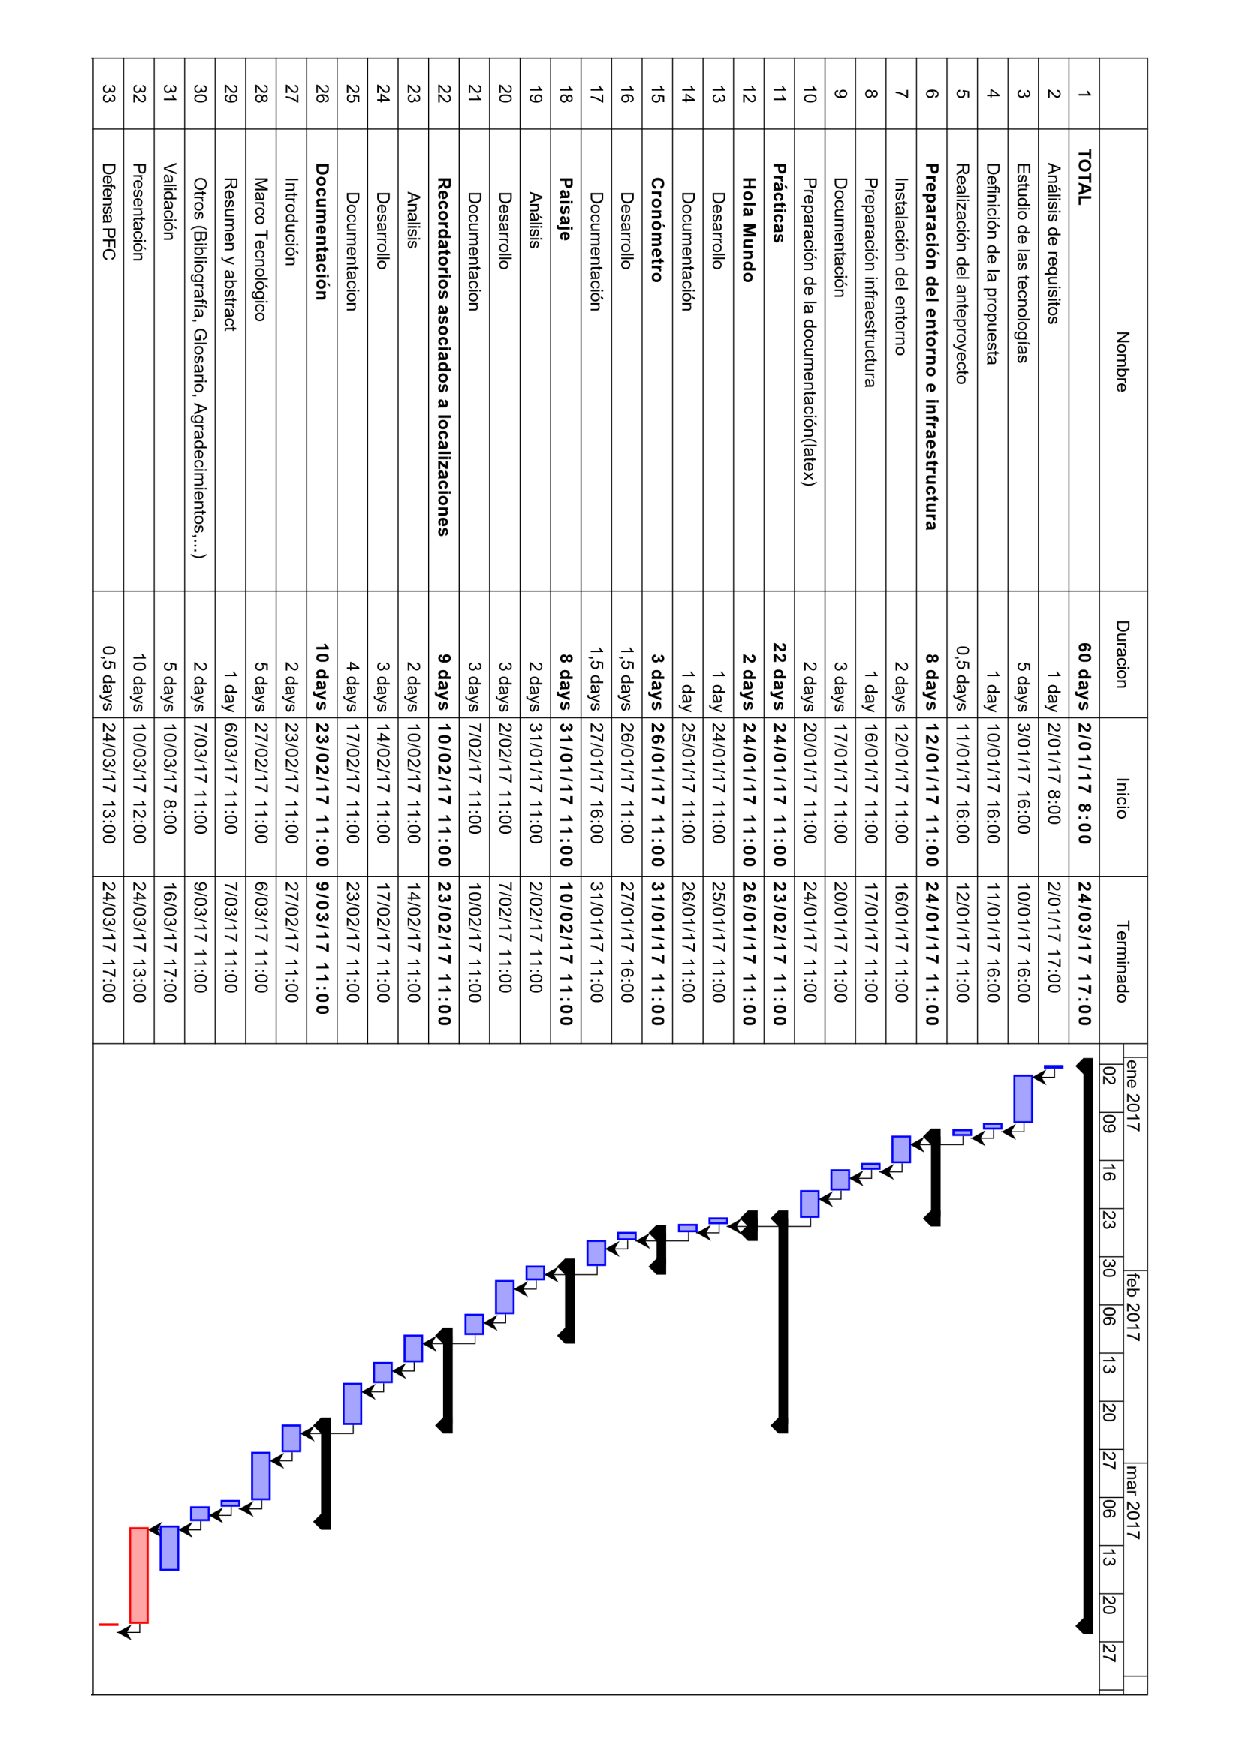
\includepdf[pages=1,scale=0.85,offset=30 -10,pagecommand={\pagestyle{fancy}}]{Presupuesto/calendar_1.pdf}
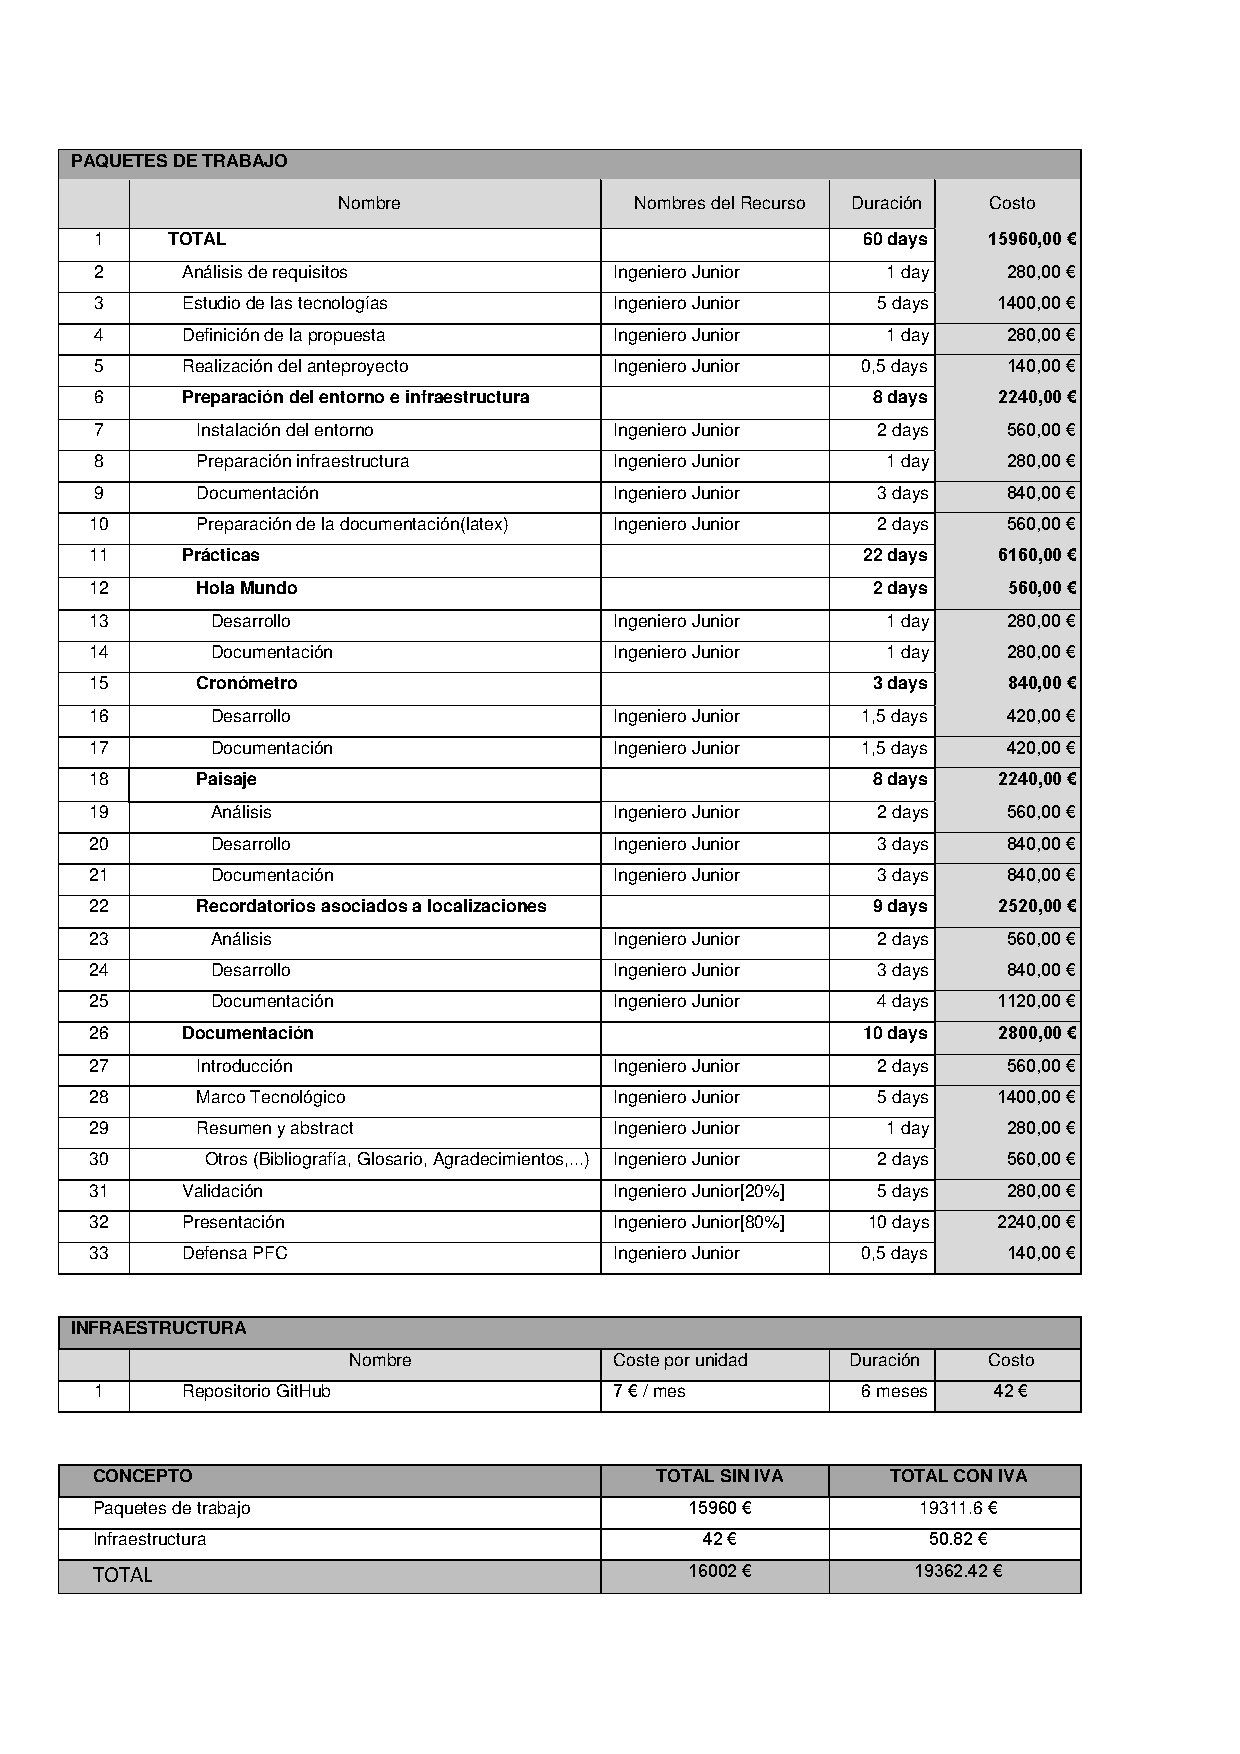
\includepdf[pages=1,scale=0.85,offset=50 20,pagecommand={\pagestyle{fancy}}]{Presupuesto/cost_1.pdf}


%------------------------------------------------------------
%          Bibliografia
%------------------------------------------------------------
\cleardoublepage
\addcontentsline{toc}{chapter}{Bibliografía}
\printbibliography
%-------------------------------------------------------------

%============================================================
%   Apéndices
%============================================================
\renewcommand{\appendixtocname}{ANEXOS}
\renewcommand{\appendixpagename}{ANEXOS}
\renewcommand{\appendixname}{ANEXOS}
\appendix
\appendixpage
\addappheadtotoc
\begin{appendices}
\addtocontents{toc}{\protect\setcounter{tocdepth}{5}}
\chapter{Herramientas para trabajar con Android} \label{ch:androidTools}

Para desarrollar una aplicación, debemos de contar con las herramientas necesarias para hacerlo, y esto no es una excepción cuando trabajamos con Android. Las herramientas más habituales son:

\begin{enumerate}
  \item Android \acrfull{SDK}: Es un conjunto de herramientas para el desarrollo de aplicaciones en Android. Comprende un depurador de código, biblioteca, emulador de terminales, documentación, ejemplos y tutoriales.
  \item \acrfull{ADB}: Aplicación incluida dentro del \gls{SDK} compuesta por tres componentes: un cliente y un servidor que se ejecutan en la máquina de desarrollo, y un daemon que se ejecuta en el termina. Esta aplicación nos permite la comunicación ya sea a través de línea de comandos (comando adb) o a través de una interfaz gráfica (consola de depuración de Google Chrome) con los dispositivos Android conectados vía \gls{USB} o que están siendo emulados.
  \item \acrfull{AVD}: Herramienta para emular dispositivos Android basada en \emph{qemu}\footnote{\url{http://www.qemu-project.org/}}
  \item Android Studio: Se trata de un \gls{IDE} basado en ItelliJ y que vino a sustituir a Eclipse como \gls{IDE} oficial a la hora de programar aplicaciones para Android.
\end{enumerate}

Para instalar estas herramientas tenemos dos opciones. Instalar tanto Android Studio como Android SDK, o descargarnos las herramientas que conforman Android SDK en caso de querer trabajar con un IDE diferente. En nuestro caso, vamos a instalar solamente Android SDK, ya que para trabajar con tecnologías web existen alternativas mejores que Android Studio.

\section{Instalación de Android SDK}

Android SDK es un conjunto de herramientas que podemos descargar en forma de fichero comprimido, por lo que más que instalar, lo que haremos será descargarnos este fichero y descomprimirlo en nuestro ordenador. Antes de ver como poder descargárnoslo y explicar algunos de sus componentes y como usarlos, vamos a explicar como instalar el \glsfirst{JDK}, software necesario para poder utilizar las herramientas de Android.

\begin{enumerate}
  \item Accedemos a la página de descarga de Java, propiedad de Oracle, \url{http://www.oracle.com/technetwork/java/javase/downloads/index.html}, donde veremos la opción de para descargarnos el \gls{JDK}.
  \item Deberemos aceptar los términos de uso y elegir la versión que necesitamos antes de empezar con la descarga.
  \begin{figure}[H]
\centering
    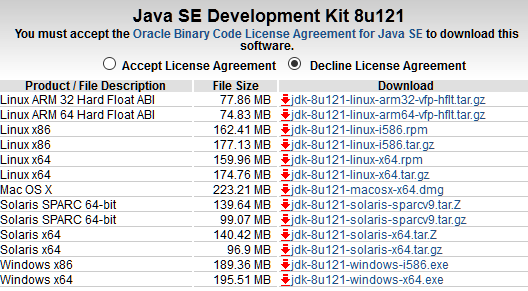
\includegraphics[width=0.8\textwidth]{Figures/anexo/android_tools/jdk_download}
    \caption{\glsfirst{JDK} está disponible para diferentes sistemas operativos y arquitecturas.}
  \end{figure}
  \item Es importante durante la instalación ver la localización donde se va a realizar, ya que puede ser necesario indicar esta ruta de instalación por si nos la requiere el SDK de Android.
  \begin{figure}[H]
\centering
    \includegraphics[width=0.8\textwidth]{Figures/anexo/android_tools/jdk_custom_setup_1}
    \caption{Durante la instalación podremos cambiar la ruta de instalación del \gls{JDK}, aunque se recomienda no modificarla si no es estrictamente necesario.}
  \end{figure}
  \item  Lo mismo ocurre con la ruta de instalación de \glsfirst{JRE}.
\end{enumerate}

Si todo ha ido bien, podremos ejecutar el comando de Java desde consola.

\begin{figure}[H]
\centering
  \includegraphics[width=0.8\textwidth]{Figures/anexo/android_tools/jdk_check}
  \caption{Podemos comprobar desde la consola la versión del \gls{JDK} que tenemos instalada.}
\end{figure}

Con el \gls{JDK} ya disponible en nuestro equipo, podemos descargarnos el \gls{SDK} de Android desde la página de desarrolladores que ofrece Google, \url{https://developer.android.com/studio/index.html#downloads}. En esta página podremos encontrar el instalador de Android Studio (opción mas destacada) y el \gls{SDK} de manera individual. De ambos existen versiones para diferentes sistemas.

\begin{figure}[H]
\centering
  \includegraphics[width=0.8\textwidth]{Figures/anexo/android_tools/sdk_download}
  \caption{Aunque la opción está un poco ``escondida'', podemos descargarnos el \gls{SDK} de Android sin necesidad de instalar Android Studio.}
\end{figure}

Cuando se haya completado la descarga, podremos descomprimir el fichero en el directorio que queramos y poder ver los componentes que forman Android \gls{SDK}.

\begin{figure}[H]
\centering
  \includegraphics[width=0.8\textwidth]{Figures/anexo/android_tools/sdk_uncompressed}
  \caption{Ficheros que se encuentran dentro del paquete comprimido.}
\end{figure}

\section{Android SDK Manager}\label{sec:SDKManager}

El paquete de Android \gle{SDK} cuenta \emph{Android SDK Manager}, que nos permite instalar las herramientas que ofrece el SDK, las plataformas y  otros componentes de manera independiente. Una vez iniciado veremos una ventana como la siguiente:

\begin{figure}[H]
\centering
  \includegraphics[width=0.8\textwidth]{Figures/anexo/android_tools/sdk_manager}
  \caption{Android SDK Manager nos permite instalar los diferentes componentes de Android SDK por separado.}
\end{figure}

Los componentes aparecen agrupados en diferentes grupos:

\paragraph{Tools} Aquí se encuentran varias herramientas indispensables para poder crear una aplicación para Android. Es recomendable instalar la última versión de aquellas que aparezcan. Los paquetes herramientas que nos encontramos son \textbf{Android SDK tools}, que contiene elementos como el emulador, \textbf{Android SDK Platform-tools}, donde se incluye \gls{ADB} y \textbf{Android SDK Build-tools}, con las herramientas que compilan y generan la aplicación.

\paragraph{Android SDK Platform} Diferentes versiones de la plataforma Android. Al menos tendremos que tener una de ellas disponible, que bien puede ser la última, lo cuál es lo más recomendable, o bien una anterior, según los requisitos del desarrollo. Aquí también se encuentran las imágenes del sistema que podremos ejecutar en el emulador.

\paragraph{Extras} Software que no se engloba en ninguno de los otros grupos pero que pueden ser de utilidad durante el desarrollo de nuestro proyecto. Aquí se podemos encontrarnos con los drivers \textbf{Google USB}, que dependiendo del dispositivo que tengamos, necesitaremos instalar para poder conectarlo a nuestro \gls{PC}; el \textbf{repositorio de Google}, con diferentes bibliotecas; o \textbf{Google Play services}.

\section{Android Virtual Device}\label{sec:AVD}

Llamamos \acrfull{AVD}\footnote{\url{https://developer.android.com/studio/run/managing-avds.html}} a la definición de características de un dispositivo Android, ya sea un teléfono, una tablet, un smartwatch, \ldots. Entre otras propiedades, se encuentra el hardware del dispositivo, la imagen del sistema o el espacio de almacenamiento asociado. Los \gls{AVD} pueden ser emulados usando \nameref{sec:AndroidEmulator}.

Para gestionar nuestros \glspl{AVD} disponemos de un manager al que podemos acceder desde el \nameref{sec:SDKManager}.

\begin{figure}[H]
\centering
  \includegraphics[width=0.8\textwidth]{Figures/anexo/android_tools/avd_open_manager}
  \caption{Desde el propio manager de Android SDK podremos abrir el manager de avds.}
\end{figure}

Esto nos abre una ventana como la siguiente en la que podemos ver dos pestañas. En una aparecerá una lista con los \glspl{AVD} disponibles, en la otra, una lista de definiciones de dispositivos.

\begin{figure}[htbp]
\centering
\subfigure[Lista de AVDs]{\includegraphics[width=0.45\textwidth]{Figures/anexo/android_tools/avd_manager_avds_list}}\hspace{0.05\textwidth}
\rulesep
\subfigure[Lista de definiciones de dispositivos]{\includegraphics[width=0.45\textwidth]{Figures/anexo/android_tools/avd_manager_definitions_list}}
\caption{AVDs Manager.}
\end{figure}

En el listado de dispositivos podemos ver algunos que vienen por defecto, entre los que encontramos terminales de la familia Nexus, Android TV, smartwatchs y tablets. Con estos dispositivos debería ser más que suficiente, pero si queremos, podemos crear los nuestros propios desde cero, o clonando alguno de los ya existentes, y así poder personalizar al gusto las características del hardware.

\begin{figure}[H]
\centering
  \includegraphics[width=0.8\textwidth]{Figures/anexo/android_tools/avd_manager_definitions_create}
  \caption{A la hora de crear un nuevo dispositivo, podemos configurar varias características de su hardware.}
\end{figure}

Por otro lado, la lista de \glspl{AVD} se encuentra vacía ya que no viene ninguna configuración establecida por defecto. Para crear la nuestra y poder emularla, pulsamos el botón \textbf{Create AVD}. Nos abrirá una ventana donde podremos configurar nuestro \gls{AVD}.

\begin{figure}[H]
\centering
  \includegraphics[width=0.6\textwidth]{Figures/anexo/android_tools/avd_manager_avds_create}
  \caption{Vista con la que podemos crear nuestro \gls{AVD}.}
\end{figure}

Los campos que debemos rellenar en este paso son:

\begin{enumerate}
  \item AVD Name: Nombre con el que identificar nuestro \gls{AVD}, tanto dentro del manager, como fuera. Este nombre será el que se utilice para identificar el emulador en herramientas externas, como Ionic CLI cuando se usa la opción \emph{emulate}.
  \item Device: Definición del dispositivo que queremos que se use. En esta lista aparecerán los dispositivos por defecto y los que hayamos creado nosotros.
  \item Target: Versión de la plataforma Android que usará. Solo aparecerán aquellas que se hayan descargado previamente desde el \gls{SDK} manager.
  \item CPU/ABI: Imagen del sistema. También tendrá que ser descargado con anterioridad junto con la versión de la plataforma desde el \gls{SDK} manager.
  \item Keyboard: Si habilitamos esta opción, el emulador entenderá que el dispositivo dispone de un teclado físico por lo que no se mostrará el teclado virtual.
  \item Skin: Aspecto que debe utilizar el dispositivo y que definirá el tamaño con el que se verán los elementos de la aplicación, como los botones.
  \item Front/Back Camera: Cámaras que tendrá el dispositivo. En caso de disponer, la imagen puede ser emulada, o utilizar una webcam conectada a nuestra máquina.
  \item Memory Option: Memoria RAM que utilizará el emulador. Debemos de configurar esta cantidad teniendo en cuenta la memoria RAM disponible en la máquina en la cual vayamos a ejecutar el emulador.
  \item Internal Storage y SD Card: Capacidad de almacenamiento que tendrá el dispositivo emulado y que podremos definir por separado según se trate del propio almacenamiento del sistema, o corresponde a una memoria extraíble.
  \item Emulation Option: Estas opciones tienen que ver con el rendimiento del emulador. La opción \emph{Snapshot} crea una ``copia'' del sistema emulado en la memoria RAM lo que acelera un posible reinicio de la aplicación. La opción \emph{Use Host GPU} como se puede uno imaginar, hace que el emulador haga uso de la tarjeta gráfica de la máquina que lo ejecuta, acelerando las operaciones relacionadas con la visualización.
\end{enumerate}

\section{Android Emulator}\label{sec:AndroidEmulator}

El emulador de Android\footnote{\url{https://developer.android.com/studio/run/emulator.html}} que ofrece Android \gls{SDK}, basado en \textbf{qemu}\footnote{\url{http://www.qemu-project.org/}}, nos permite emular nuestros \glspl{AVD} y ejecutar dentro las aplicaciones Android que desarrollamos.

El emulador nos permite además, simular diferentes características de las que dispone el dispositivo real y con los que no contamos en la máquina de desarrollo. Un ejemplo son las cámaras con las que cuentan la mayoría de dispositivos, y que como vimos en la creación de \glspl{AVD}, podemos simular.

\begin{figure}[H]
\centering
  \includegraphics[width=0.45\textwidth]{Figures/anexo/android_tools/emulator}
  \caption{Emulador de Android, con la pantalla a la izquierda y la botonera a la derecha.}
\end{figure}

Al ejecutar el emulador nos aparece por un lado una ventana que simula la pantalla del dispositivo, y por otro una barra vertical con botones. La pantalla actua como la de un dispositivo real en la que el puntero del ratón hace de dedo. El gesto de pellizco, en el cual se usan dos dedos, se puede simular pulsando la tecla Ctrl o Command (⌘). Además, si arrastramos nuestra \gls{APK} sobre esta pantalla, el emulador instalará la aplicación en el simulador; en caso de arrastrar otro tipo de archivos, este se almacenará como un fichero dentro del sistema emulado.

En la barra vertical contamos con diferentes funciones típicas de un terminal móvil y que se suelen reflejar mediante un botón físico o software en los terminales reales. Ejemplo de esto es el botón de apagado, los de volumen, la botonera inferior característica de Android (que según el modelo de dispositivo, son implementados vía software o mediante botones físicos), \ldots.

Al final de la barra vertical se encuentra un botón con el cual podremos abrir los controles extendidos.

\begin{figure}[H]
\centering
  \includegraphics[width=0.8\textwidth]{Figures/anexo/android_tools/emulator_extended_controls}
  \caption{Ventana de controles extendidos del emulador.}
\end{figure}

Desde esta ventana podremos simular diferentes sensores, llamadas, estado de la batería, \ldots.

\chapter{Instalar Node.JS y npm}
Desde la versión 0.6.3 de Node.JS, el gestor de paquetes \gls{npm} se instala junto al mencionado entorno de ejecución. En esta sección, se explicarán los pasos a seguir para intalar Node.JS en una máquina con sistema operativo Windows.

\begin{enumerate}
\item Lo primero que debemos hacer es descargar el instalador de Node.JS. Esto lo podemos hacer desde la web oficial de Node.JS (\url{https://nodejs.org/es/download/}). Podremos escoger entre descargarnos la versión \gls{LTS}, que en el momento de escribir este documento se corresponde a la versión 6.9.2, que incluye la versión 3.10.9 de \gls{npm}; o la versión mas actualizada, Node.JS versión 7.2.0 junto con la 3.10.9 de \gls{npm}. Para este manual, hemos escogido la versión mas actual (7.2.0) para Windows x64 en su formato binario (.exe).
\item Una vez descargado el binario, lo ejecutamos apareciéndonos la bienvenida al instalador de node.JS.
\begin{figure}[H]
\centering
  \includegraphics[width=0.8\textwidth]{Figures/anexo/anexoI/nodejs/1}
  \caption{Paso de bienvenida del instalador.}
\end{figure}
\item Pulsamos el botón siguiente, lo que nos llevará a una pantalla con los términos de uso.
\begin{figure}[H]
\centering
  \includegraphics[width=0.8\textwidth]{Figures/anexo/anexoI/nodejs/2}
  \caption{Terminos de uso.}
\end{figure}
\item En el siguiente paso nos permitirá seleccionar la ruta de instalación. Bajo esta ruta se instalarán los scripts ejecutables, por lo que será necesaria recordarla en caso de tener que configurar manualmente las variables de entorno de Windows.
\begin{figure}[H]
\centering
  \includegraphics[width=0.8\textwidth]{Figures/anexo/anexoI/nodejs/3}
  \caption{Configuración del directorio de instalación de node.JS.}
\end{figure}
\item Por último nos aparecerá una ventana en la que ya iniciar el proceso de instalación. Será necesario otorgarle permisos de administrador para que pueda realizar la instalación.
\begin{figure}[H]
\centering
  \includegraphics[width=0.8\textwidth]{Figures/anexo/anexoI/nodejs/4}
  \caption{Paso final.}
\end{figure}
\end{enumerate}

Una vez completada la instalación, podremos hacer uso tanto de Node.JS como de npm a través de Windows PowerShell (o de la consola de comandos) o de programas de terceros que hagan uso de estas herramientas.
Para comporbar que la instalación se ha realizado correctamente, desde Windows PowerShell comprobamos la versión de los programas instalados y ejecutamos un pequeño código JavaScript.

\begin{figure}[H]
\centering
  \includegraphics[width=0.8\textwidth]{Figures/anexo/anexoI/nodejs/6}
  \caption{La instalación se ha realizado correctamente.}
\end{figure}

Si el sistema no es capaz de reconocer los comando node o npm, tendremos que chequear que el directorio en el que se realizó la instalación se encuentra configurado en las variables de entorno de Windows. Desde Windows PowerShell se pueden ver estas variables con el siguiente comando:

\begin{lstlisting}[language=bash]
  # Get-ChildItem Env:
\end{lstlisting}
o para ver en más detalle la variable PATH:
\begin{lstlisting}[language=bash]
  # \$Env:PATH
\end{lstlisting}

Si vemos que el directorio de instalación no aparece, tendremos que configurarlo manualmente:
\begin{lstlisting}[language=bash]
  # \$env:Path += ";C:\path\to\node"
\end{lstlisting}

\chapter{Atom} \label{ch:atom}

A la hora de decidir que editor utilizar, influye los gustos de cada uno.  Actualmente existe un catálogo enorme de editores, tanto gratuitos como de pago, los cuales ofrecen la mayoría de funcionalidades básicas que podemos esperar de en un editor.
La propia página de Ionic \footnote{\url{https://ionicframework.com/docs/v2/resources/editors_and_ides/}} nos recomiendan los siguientes basándose en el soporte que ofrecen a la hora de trabajar con este framework:
\begin{itemize}
\item Visual Studio Code
\item Atom
\item WebStorm
\item ALM
\item Angular IDE by Webclipse
\end{itemize}

\tipbox{Es importante también a la hora de elegir un editor, como se adapta este al resto de lenguajes que utilicemos, sin tener que tener abierto un editor por cada lenguaje y poder manejar con solo uno todo el proyecto.}

Para la realización de este \gls{PFC} vamos he escogido como editor Atom. Vengo usando este editor desde hace ya un tiempo no solo para programación en HTML y JS, si no también para otros lenguajes como Python o SQL y escribir textos con \LaTeX (como por ejemplo esta memoria).
Atom es un editor de código abierto para Windows, Linux y MacOS desarrollado por GitHub (el código fuente se puede descargar desde su repositorio \footnote{\url{https://github.com/atom/atom}}. Aún siendo una aplicación de escritorio, esta desarrollado utilizando tecnologías web, más concretamente Chronium y NodeJS. Esto da lugar a uno sus puntos fuertes, que es la personalización de la aplicación; como muy bien indican en su página, Atom es: \say{A hackable text editor for the 21st Century}.

\section{Instalación}

Como hemos comentado, Atom se encuentra disponible para los sistemas Windows, Linux y MacOS. Desde su propio repositorio en GitHub podemos descargarnos cualquiera de las versiones disponibles para cada uno de los sistemas antes mencionados (\url{https://github.com/atom/atom/tags}).

\section{Personalización}

Como ya se ha comentado, uno de los puntos fuertes de Atom es la personalización, permitiendo al propio usuario tener su propia configuración o utilizar recursos creados por terceros.

\subsection{Paquetes y temas}

Una característica habitual de las aplicaciones de código abierto es permitir a los usuarios crear y compartir modificaciones de la aplicación, y como no, Atom no podía ser menos. Estas modificaciones se agrupan en dos tipos:

\begin{itemize}
  \item Los \textbf{paquetes (packages)}, los cuales añaden nuevas funcionalidades al editor,
  \item y los \textbf{temas (themes)}, que cambian el aspecto visual de la aplicación.
\end{itemize}

Para ambos existe un listado donde encontrarlos en loa propia web de Atom (\url{https://atom.io/packages} y \url{https://atom.io/themes}), o más facil aún, desde la la propia configuración de la aplicación (File > Settings > Install).

\begin{figure}[H]
\centering
  \includegraphics[width=0.8\textwidth]{Figures/anexo/anexoI/atom/install_packages_and_themes}
  \caption{Pantalla desde donde instalar paquetes y temas desde la propia aplicación de atom.}
\end{figure}

\chapter{Ionic}\label{ch:ionic}
Al tratarse de un paquete nodeJS, Ionic puede ser instalado usando \gls{npm} de una manera muy sencilla. A continuación detallaremos los pasos a seguir, asumiendo que en la máquina en la que estamos trabajando se encuentra instalado nodeJS y npm (ver anexo).
\begin{itemize}
  \item En primer lugar instalaremos Cordova, usando también para ello \gls{npm}. Para ello ejecutaremos el siguiente comando.
  \begin{lstlisting}[language=bash]
    # npm install -g cordova
  \end{lstlisting}
  El proceso puede tardar unos minutos ya que tendrá que instalar varias dependencias.
  \item Una vez instalado Cordoba, procedemos a la instalación de ionic.
  \begin{lstlisting}[language=bash]
    # npm install -g ionic
  \end{lstlisting}
\end{itemize}

\notebox{Existen dos maneras de instalar paquetes con \gls{npm}, de manera global o de manera local. Si queremos utilizar el paquete como una herramienta vía línea de comandos, debemos instalarla de manera global; en cambio, si queremos que el paquete sea una dependencia del modulo que estamos programando, debemos instalarlo de manera local. La opción \emph{--global/-g} indica a \gls{npm} que el paquete debe ser instalado de manera global ya que por defecto lo instalará de manera local.}

Para probar que se ha instalado de manera correcta, probaremos crearemos un nuevo proyecto y probaremos que funciona.
\begin{itemize}
  \item Dentro de nuestro área de trabajo, crearemos un nuevo proyecto utilizando para ello el comando \emph{ionic start} seguido del nombre de nuestro proyecto.
  \begin{lstlisting}[language=bash]
    # ionic start --v2
  \end{lstlisting}
  \item El anterior comando creará un nuevo directorio con el mismo nombre del proyecto. Dentro de este directorio descargará una templete por defecto, por lo que dentro encontraremos diferentes ficheros y directorios:
  \begin{figure}[H]
\centering
    \includegraphics[width=0.8\textwidth]{Figures/anexo/anexoI/ionic/ionic_start}
    \caption{Estructura de archivos que sirve como base para empezar un nuevo proyecto con ionic. Han sido generados utilizando el comando \emph{ionic start}.}
  \end{figure}
  \item Podemos hacer que ionic ponga en marcha un servidor de desarrollo para poder acceder a la aplicación a través de un browser. Solo tenemos que ejecutar el comando \emph{ionic serve} dentro del directorio anterior. Aparecerá un mensaje indicando que el servidor está levantado además de cierta información como la url para acceder a la aplicación, los ficheros que está sirviendo o los comandos para realizar ciertas acciones.
  \begin{figure}[H]
\centering
    \includegraphics[width=0.8\textwidth]{Figures/anexo/anexoI/ionic/ionic_serve}
    \caption{Vemos como el servidor de la aplicación ionic está en marcha.}
  \end{figure}
  \item Si abrimos nuestro navegador y accedemos a la url que indica el servidor (por defecto será la IP de la máquina y el puerto 8100), veremos la aplicación servida, que no es más que el template descargado anteriormente:
  \begin{figure}[H]
\centering
    \includegraphics[width=0.8\textwidth]{Figures/anexo/anexoI/ionic/its_alive}
    \caption{La aplicación vista desde un navegador.}
  \end{figure}
\end{itemize}

\chapter{Google APIs}\label{ch:google_api}

Se conoce por este nombre al conjunto de \glspl{API} desarrolladas por Google y que permiten a aplicaciones de terceros acceder a los servicios de Google, como pueden ser Search, Google Map, Google Traslator, Gmail, \ldots. El uso de estas \glspl{API} suelen estar limitado a un número de peticiones diarias, acarreando un coste adicional todas aquellas que superen este límite.

Para poder hacer uso de estas \glspl{API} es necesario autorización y autenticación, es por ello necesario crear antes una cuenta en Google para poder obtener las credenciales con las que autenticarnos ante los servicios de Google. Si ya disponemos de una cuenta en Google, podremos acceder a la consola para desarrolladores\footnote{\url{https://console.developers.google.com}}. Desde esta consola podremos realizar diferentes gestiones sobre nuestra cuenta.

\begin{figure}[H]
\centering
  \includegraphics[width=0.8\textwidth]{Figures/anexo/google_api/developer_console}
  \caption{Consola para desarrolladores de Google.}
\end{figure}

A nuestra cuenta le podemos asignar varios proyectos. Esto nos ayudará a gestionar por separado las credenciales que generemos y poder diferenciar el uso que se le ha dado a cada una de ellas (consumo, número de peticiones, acceso a servicios, \ldots). Esto es útil en caso de tener varias aplicaciones, o simplemente tener una sola aplicación, pero varios entornos (desarrollo, preproducción, producción, piloto, \ldots)

\section{Obtención de una clave para utilizar Google Maps}

Para la realización de una de las prácticas propuestas, va a ser necesario el uso de una clave, \emph{API KEY}, que permita a nuestra aplicación hacer uso del servicio de Google Maps. Vamos a ver como podemos conseguir esta clave. Daremos por supuesto que disponemos de una cuenta de Google a la cual vincularemos nuestro proyecto.

\warningbox{
  Tened en cuenta que el uso de estas \glspl{API} pueden incurrir en costes que serán cargados a la cuenta a la que este asociado el proyecto. Debemos ser cautelosos con el uso que hacemos des de estas claves, y en caso de no necesitarlas, destruirlas.
}

En primer lugar, crearemos un proyecto dentro de nuestra cuenta. Le asignaremos un nombre para poder identificarlo, y si lo deseamos, podremos modificar el ID que asigna Google automáticamente.

\begin{figure}[H]
\centering
  \includegraphics[width=0.8\textwidth]{Figures/anexo/google_api/create_project}
  \caption{Ventana para la creación de un proyecto dentro de nuestra cuenta.}
\end{figure}

Una vez creado, podremos verlo en la lista con el resto de proyectos y podremos seleccionarlo.

\begin{figure}[H]
\centering
  \includegraphics[width=0.8\textwidth]{Figures/anexo/google_api/project_list}
  \caption{Lista de proyectos asociados a nuestra cuenta.}
\end{figure}

Si desplegamos el menú lateral, podremos ver diferentes secciones relativas a nuestro proyecto, dentro de estas secciones a su vez nos encontraremos diferentes apartados, de los cuales, veremos los más importantes.

\begin{figure}[H]
\centering
  \includegraphics[width=0.6\textwidth]{Figures/anexo/google_api/menu_console}
  \caption{Menú desde el que acceder a diferentes secciones relativas al proyecto.}
\end{figure}

Si accedemos a la sección \textbf{Administrador de APIs}, podremos ver el \textbf{Panel de control}. En este panel aparecerán las estadísticas de uso de los diferentes servicios asociados. Recién creado el proyecto, esta pantalla debería aparecer vacía. Si abrimos la \textbf{Biblioteca}, veremos una lista con los diferentes servicios de Google. Aqui seleccionaremos los servicios que queremos habilitar para nuestro proyecto.

\begin{figure}[H]
\centering
  \includegraphics[width=0.8\textwidth]{Figures/anexo/google_api/api_library}
  \caption{APIs disponibles para poder asignar al proyecto.}
\end{figure}

A nosotros nos interesa el servicio \textbf{Google Maps Android API}. Lo seleccionamos y nos aparecerá una pantalla con una pequeña explicación del servicio y un botón con el que habilitarlo.

\begin{figure}[H]
\centering
  \includegraphics[width=0.8\textwidth]{Figures/anexo/google_api/api_google_map}
  \caption{Información relativa a la API de Google Maps Android.}
\end{figure}

Tras ello nos abrirá de nuevo el panel de control, esta vez, podremos ver las gráficas que nos ofrecen, que aun estando vacías, podremos hacernos una idea de la información que ofrecerán.

El siguiente paso será crear nuestra clave. Lo podremos apartado \textbf{Credenciales}, en la que veremos que al crear una, nos ofrecerá varias opciones, entre ellas, la de generar una clave que es la que nos interesa.

\begin{figure}[H]
\centering
  \includegraphics[width=0.8\textwidth]{Figures/anexo/google_api/api_credential}
  \caption{Configuración de las credenciales para nuestra API. El servicio nos proporciona diferentes maneras para realizar la autorización.}
\end{figure}

Una vez creada, nos aparecerá para poder copiarla (aunque podremos consultarla cuando queramos desde la consola) y nos dará la opción de restringir el acceso. Esta opción es muy interesante, especialmente una vez puesta en producción, ya que nos permitirá limitar quien hace uso de ella ya sea mediante una dirección \gls{IP}, una URL, el nombre del paquete de una aplicación de Android, \ldots. Si no ponemos esta restricción, alguien podría obtener la clave desde el código (por ejemplo depurando la aplicación) y utilizarla para su propia aplicación cargandonos a nosotros con los costes de uso.

\begin{figure}[H]
\centering
  \includegraphics[width=0.7\textwidth]{Figures/anexo/google_api/api_credential_restriction_options}
  \caption{Opciones para restringir el acceso según el origen de la petición. Para una aplicación Android, necesitariamos indicar el nombre del paquete de nuestra aplicación.}
\end{figure}

De vuelta al menú lateral, si nos vamos a la sección \textbf{IAM y administración}, podemos destacar el apartado \gls{IAM}, donde podremos dar permisos sobre el proyecto a otros usuarios, por ejemplo, permisos de edición, de lectura, sobre la facturación, \ldots

\begin{figure}[H]
\centering
  \includegraphics[width=0.8\textwidth]{Figures/anexo/google_api/iam}
  \caption{Permisos sobre el proyecto para distintos usuarios de la consola de desarrolladores. Aquí podemos compartir el proyecto con el resto del equipo de desarrollo y asignarles diferentes permisos a cada uno.}
\end{figure}

Y el apartado de \textbf{Cuotas}, donde vemos las cuotas de los servicios activados y podremos limitarlas.

\begin{figure}[H]
\centering
  \includegraphics[width=0.8\textwidth]{Figures/anexo/google_api/quota}
  \caption{Cuotas que se aplican a cada uno de los servicios asociados al proyecto.}
\end{figure}

\end{appendices}

\end{document}
